\clearpage
\section{Questões}
\label{sec:questoes}
\subsection{\bf{Sistemas}}
\label{subsec:sistemas}
%------------------------------------------------------%
\subsubsection{(R1) Linearidade}
\label{subsubsec:R1}
\paragraph{Resposta:} %{{
Um sistema é dito \textit{linear} se e somente se, satisfizer as seguintes propriedades:
\begin{enumerate}
    \label{propriedade:1}
    \item \underline{Sobreposição} - se um sinal \((x_1 + x_2)\) for aplicado ao sistema, então o sinal de saída será \(y_1 + y_2\). Equivalentemente pode ser visto como: se aplicarmos os sinais \(x_1\), \(x_2\), ..., \(x_i\) simultaneamente no sistema, então a saída será a soma das saídas obtidas individualmente, de cada sinal de entrada.
        \[ \text{se}\ x_1(t) \xrightarrow[]{\text{S}} y_1(t)\ \text{e}\ x_2(t) \xrightarrow[]{\text{S}} y_2(t) \implies x_1(t) + x_2(t) \xrightarrow[]{\text{S}} y_1(t) + y_2(t) \text{,} \]
        para um número arbitrário de sinais de entrada.
    \label{propriedade:2}
    \item \underline{Homogeneidade} - se um sinal \(k \cdot x_1\) for aplicado ao sistema, então o sinal de saída será \(k \cdot y_1\)\ em que \(k \in \mathbb{C}\).
        \[ \text{se}\ x_1(t) \xrightarrow[]{\text{S}} y_1(t) \implies k \cdot x_1(t) \xrightarrow[]{\text{S}} k \cdot y_1(t) \text{,}\ \forall k \in \mathbb{C} \]
\end{enumerate}

Ora, feita a analise do \(sistema_2\) fornecido foi de imediata conclusão que \textbf{não se trata de um sistema linear}. Vejamos os seguintes casos:

\begin{figure}[ht] 
    \begin{subfigure}[b]{0.5\linewidth}
        \centering
        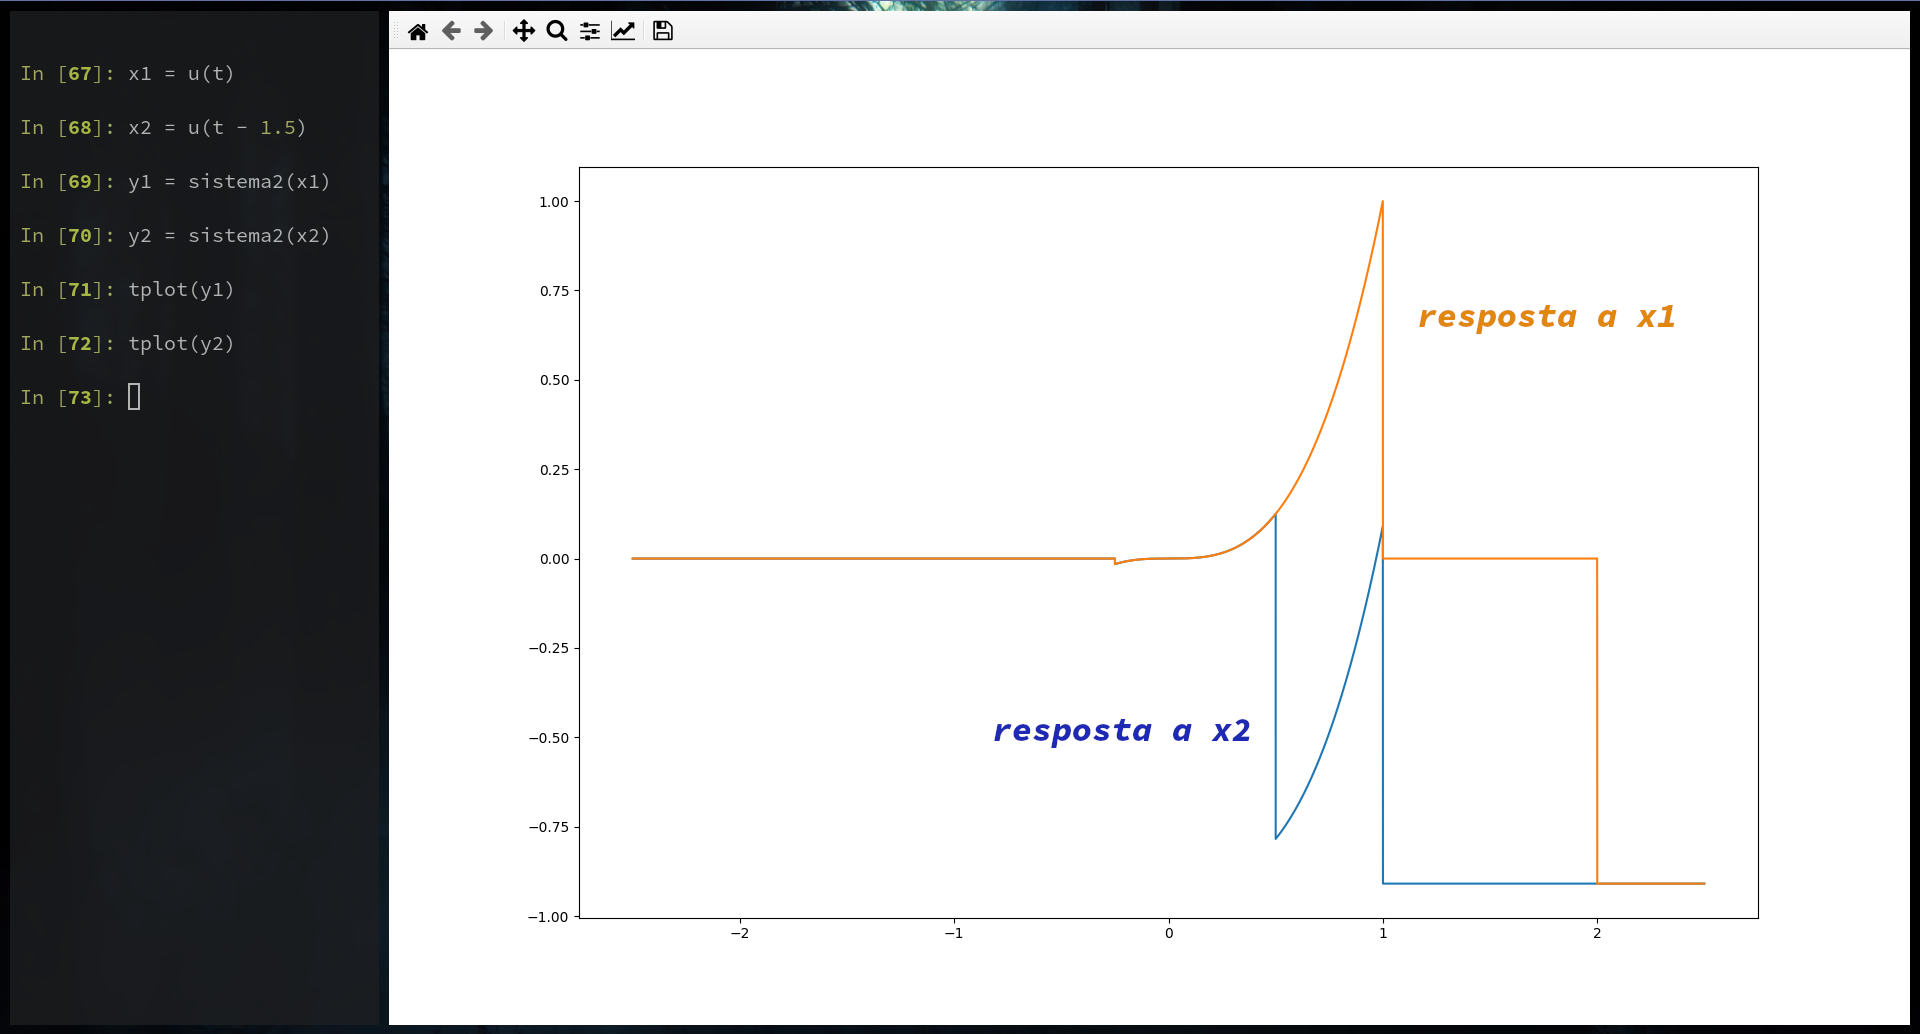
\includegraphics[width=1\linewidth]{prints/linearidade1.png}
        \caption{Resposta individual aos sinais \(x_1\) e \(x_2\)} 
        \label{fig:a} 
        %%\vspace{4ex}
    \end{subfigure}%% 
    \begin{subfigure}[b]{0.5\linewidth}
        \centering
        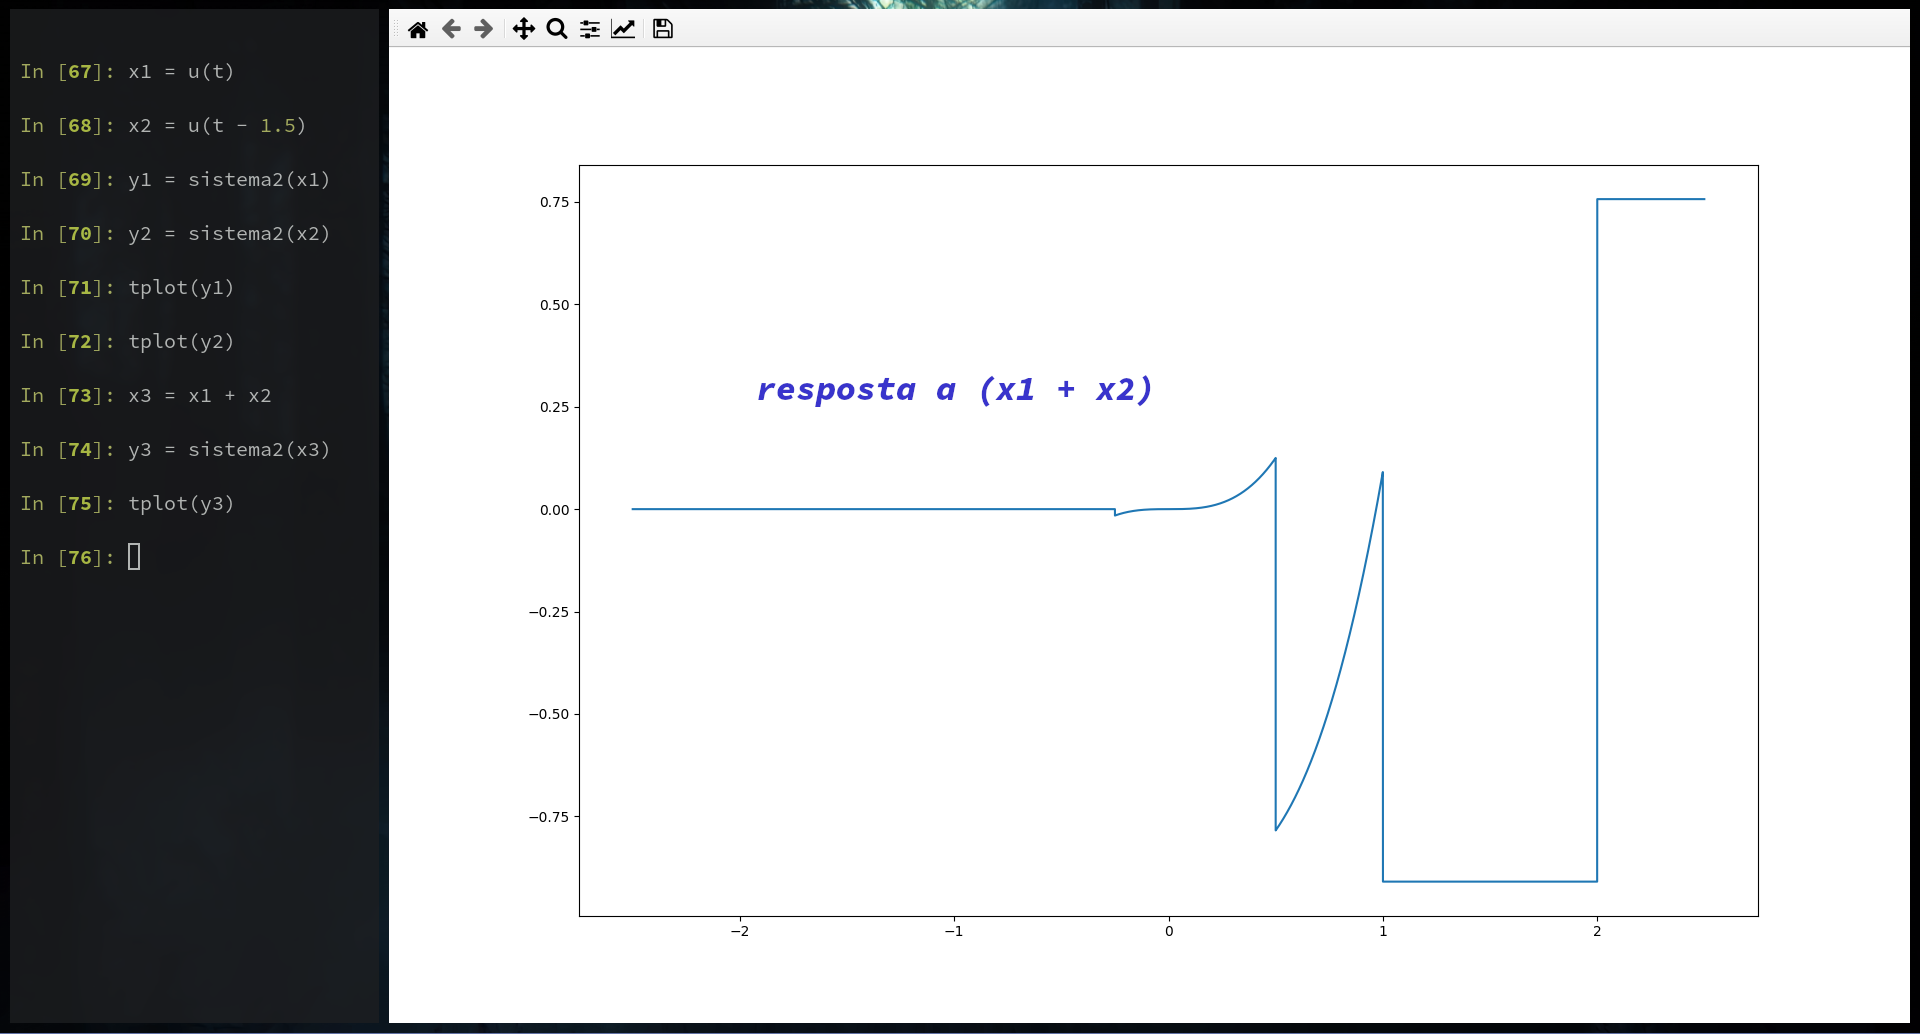
\includegraphics[width=1\linewidth]{prints/linearidade2.png} 
        \caption{Resposta à soma dos sinais de entrada} 
        \label{fig:b} 
        %%\vspace{4ex}
    \end{subfigure} 
    \caption{Exemplo onde a sobreposição não se aplica no \(sistema_2\).}
    \label{fig:multiplas}
\end{figure}

Na \hyperref[fig:multiplas]{Fig. 1} é evidente que o \(sistema_2\) falha imediatamente na primeira propriedade enunciada.

Verificou-se que a soma de dois sinais distintos, \(x_1(t) = u(t)\ \text{e}\ x_2(t) = u(t-1.5)\), que produzem respetivamente os sinais de saída distintos, \(y_1(t)\ \text{e}\ y_2(t)\), não é de todo, a soma de \(y_1(t)\ \text{com}\ y_2(t)\).

\clearpage
Foi efetuado outro teste pertinente para testar a linearidade do sistema desconhecido: 
\begin{itemize}
    \item Observar o sinal de saída para um determinado sinal de entrada e depois verificar o que aconteceria ao sinal de saída ao multiplicarmos o mesmo sinal de entrada por \(0\).
\end{itemize}

O resultado foi bastante interessante, e confirmou mais uma vez a tese de que o \textbf{\(sistema_2\) não é linear}\footnotemark[1]. No segundo instante da experiência não foi obtido um \(y_2(t) = 0,\ \forall t\) (\textit{vide} a \hyperref[propriedade:2]{propriedade 2} enunciada) como seria evidente num sistema linear.

\begin{figure}[ht]
    \centering
    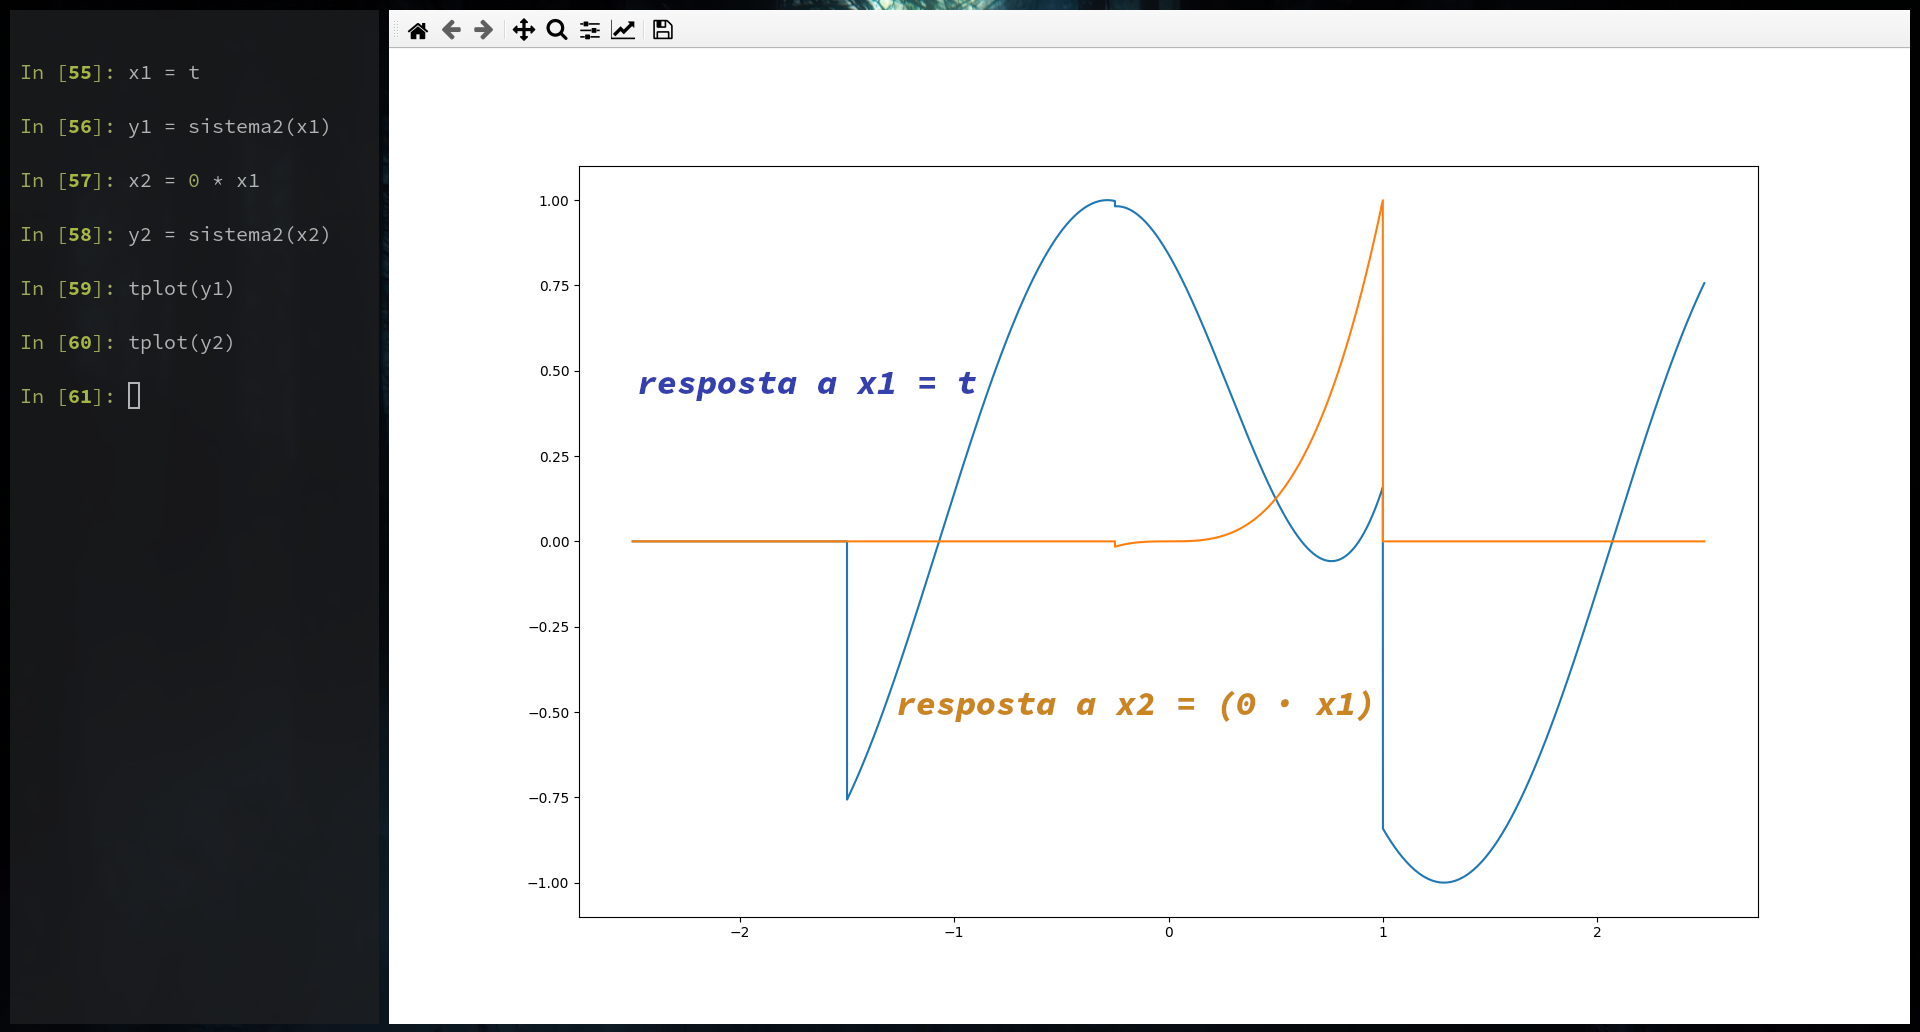
\includegraphics[width = 0.5\linewidth]{prints/linearidade3.png}
    \caption{Exemplo onde a homogeneidade não se aplica no \(sistema_2\).}
    \label{fig:homogeneidade}
\end{figure}
 
Note-se que bastava que apenas uma das propriedades referidas não se verificasse para que o sistema não fosse linear.

\footnotetext[1]{Com esta conclusão bastante marcante, ficamos impossibilitados de aplicar as técnicas de análise das propriedades de SLIT's (Sistemas \textit{Lineares} e Invariantes no Tempo) logo à partida. E como veremos no seguinte tópico \hyperref[subsubsec:R2]{(R2)}, o sistema também não é invariante no tempo (duas propriedades que facilitariam bastante a análise dos tópicos subsequentes).}

%}}
\clearpage
%------------------------------------------------------%
\subsubsection{(R2) Invariância no tempo}
\label{subsubsec:R2}
\paragraph{Resposta:} %{{
Conceptualmente, um sistema é \textit{invariante no tempo} se o comportamento e caracteristicas do sistema forem fixos ao longo do tempo.

A propriedade de invariância no tempo pode ser trivialmente descrita em termos de sinais e da linguagem de sistemas abordada. Um sistema diz-se invariante no tempo se um deslocamento do tempo no sinal de entrada resultar num deslocamento identico do tempo no sinal de saída.

    \[ \text{se}\ x_1(t) \xrightarrow[]{\text{S}} y_1(t) \implies x_1(t-t_0) \xrightarrow[]{\text{S}} y_1(t-t_0) \text{,}\ \forall t_0 \]

Ora, foi observado, coincidentemente, na questão \hyperref[fig:a]{(R1)} um caso em que a propriedade enunciada não se verifica.  O \(sistema_2\) \textbf{não se trata de um sistema invariante no tempo}.

\begin{figure}[ht]
    \centering
    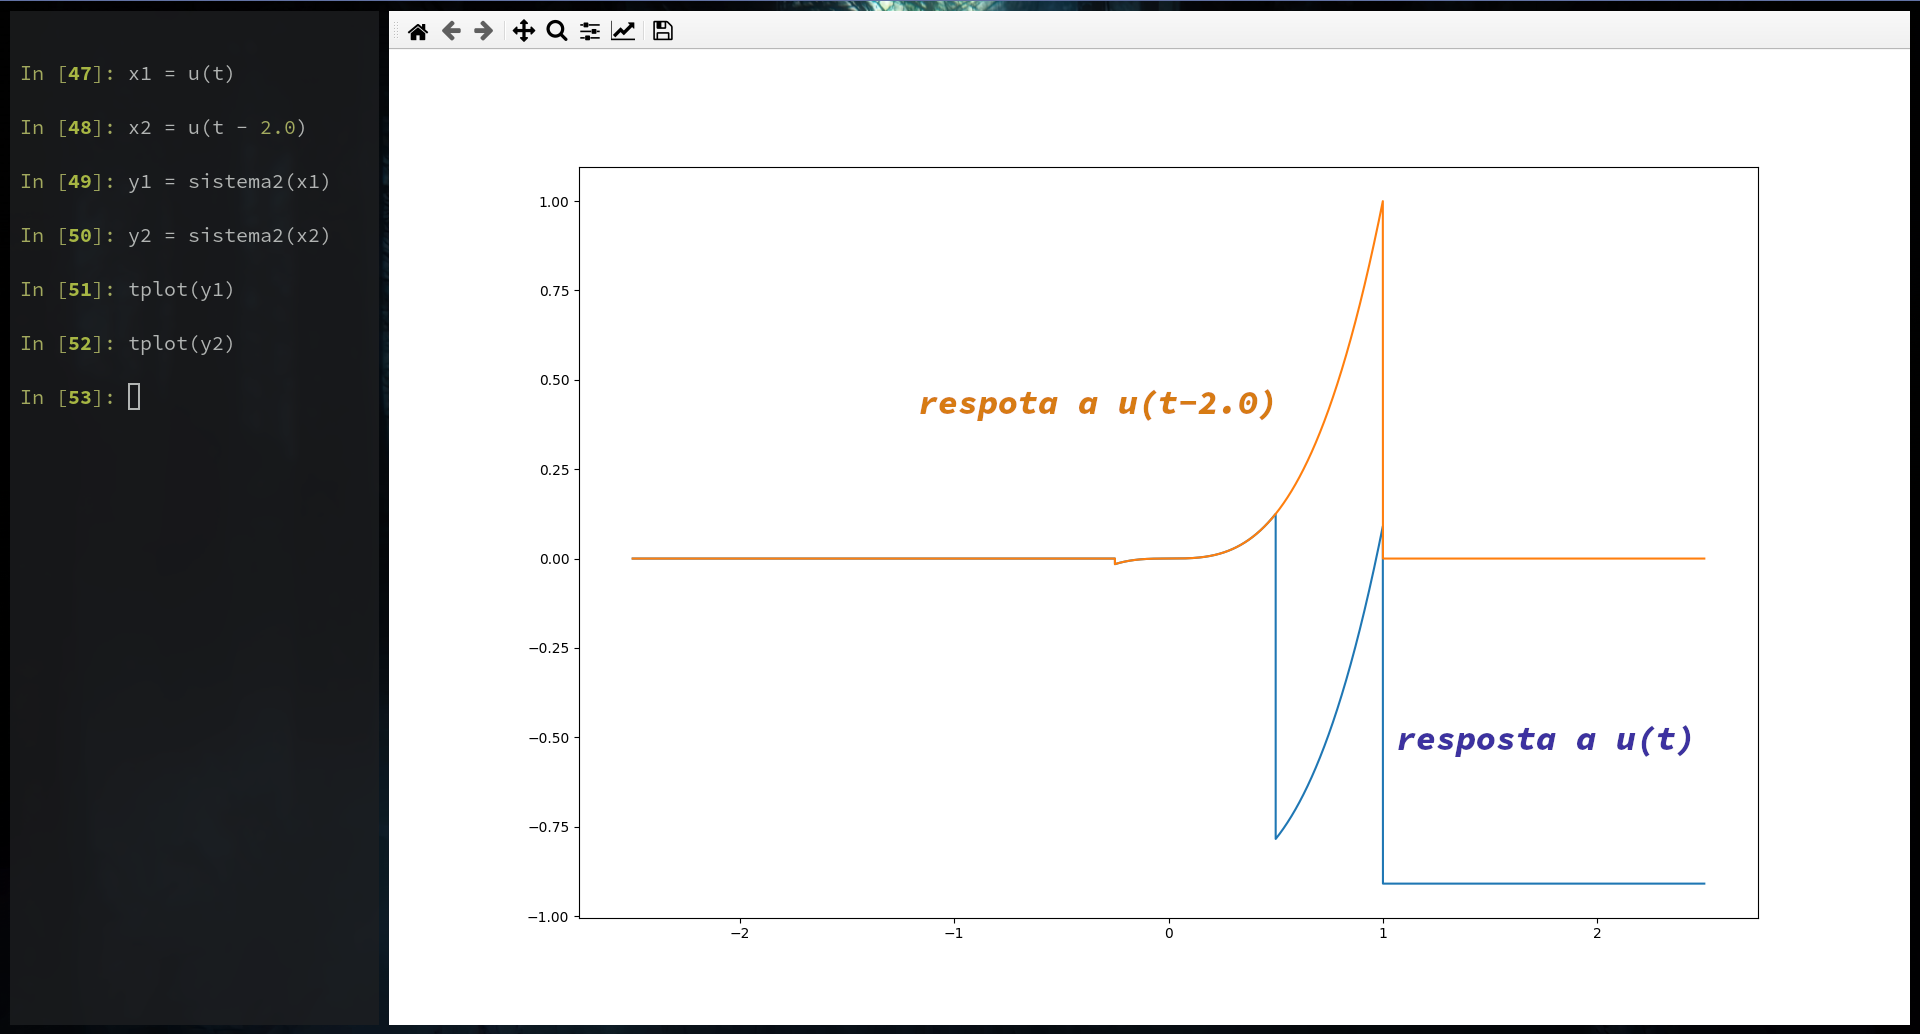
\includegraphics[width = 0.5\linewidth]{prints/variancia.png}
    \caption{Exemplo onde é evidente que o \(sistema_2\) \textbf{não é} invariante no tempo.}
    \label{fig:timeshift}
\end{figure}

Neste caso, é possível observar que após o deslocamento do degrau unitário, i.e. \(u(t - 2)\), o sinal de saída respetivo (\hyperref[fig:timeshift]{\textcolor{Orange}{a laranja}}) difere drasticamente do sinal de saída relativo ao degrau unitário (\hyperref[fig:timeshift]{\textcolor{Blue}{a azul}}). A propriedade enunciada é claramente incumprida pelo sistema.
%}}
%------------------------------------------------------%
\subsubsection{(R3) Memória}
\label{subsubsec:R3}
\paragraph{Resposta:} %{{
É dito \textit{sem memória} o sistema em que o sinal de saída, para cada valor da variável independente, a um determinado instante, apenas depende do sinal de entrada no mesmo exato instante de tempo. (Um sistema sem memória também se diz instantâneo).

Pode-se então concluir, que num sistema sem memória, dois sinais de entrada que se cruzam no instante \(t_0\), produzem sinais de saída, através do sistema, que se cruzam precisamente no instante \(t_0\).

É fácil deduzir esta conclusão se pensarmos que num sistema sem memória, o sinal de saída a cada instante depende apenas do sinal de entrada nesse mesmo instante, pelo que o cálculo da saída pode ser feito "ponto a ponto", daí, se dois sinais de entrada se intersetam no instante \(t_0\), então as suas saídas também se intersetam nesse mesmo instante \(t_0\).

\clearpage

\begin{figure}[H]
    \centering
    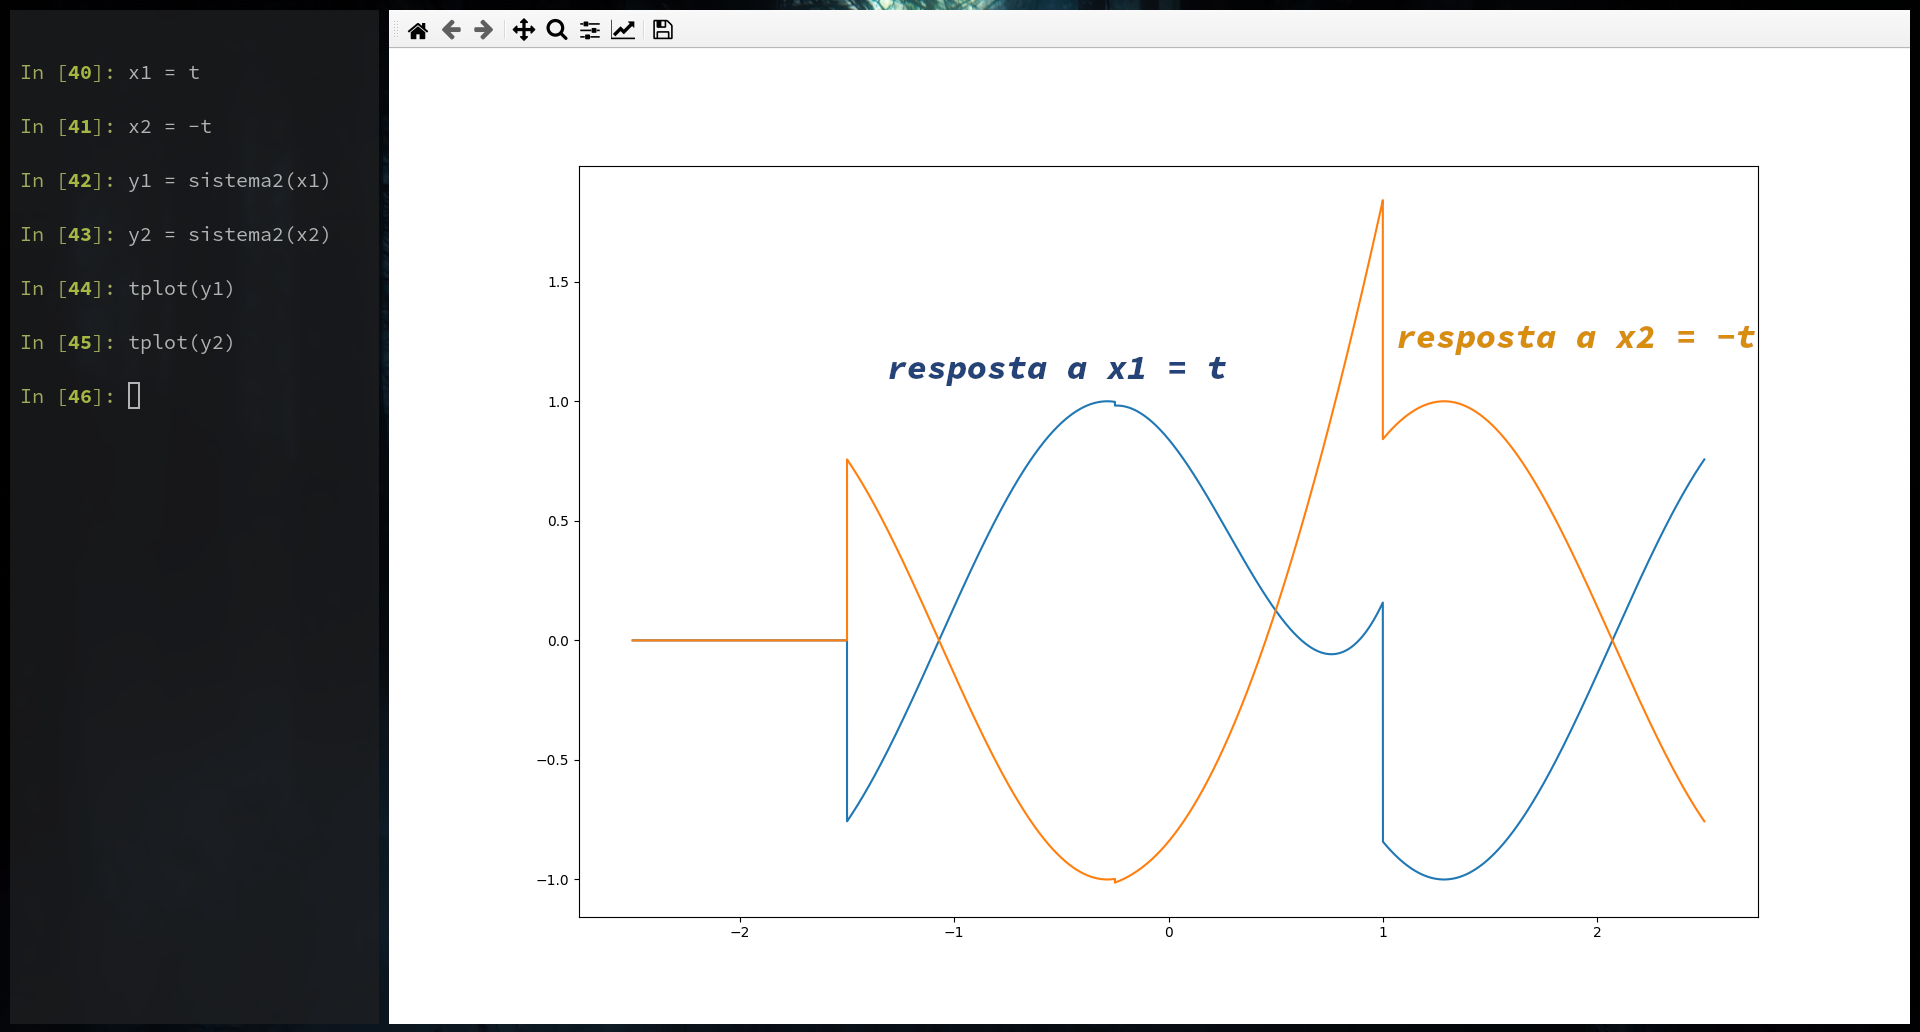
\includegraphics[width = 0.5\linewidth]{prints/memoria.png}
    \caption{Exemplo que demonstra o uso de memória do \(sistema_2\).}
    \label{fig:memory}
\end{figure}

Utilizando, como exemplo, os sinais \(x_1(t) = t\ \text{e}\ x_2(t) = -t\), que se cruzam em \(t_0 = 0\). Observando a resposta do \(sistema_2\) a ambos os sinais de entrada, i.e., \(y_1(t)\) e \(y_2(t)\), é evidente que as saídas não se cruzam em \(t_0 = 0\), como é possível constatar na \hyperref[fig:memory]{Fig. 4}. Deste modo concluímos que \textbf{o sistema tem memória}.
%}}
%------------------------------------------------------%
\subsubsection{(R4) Causalidade}
\label{subsubsec:R4}
\paragraph{Resposta:} %{{
Um sistema é \textit{causal} se o sinal de saída em qualquer instante de tempo apenas dependa do sinal de entrada no tempo presente e/ou no passado. Estes sistemas são também referidos como não antecipativos, visto que o sinal de saída não antecipa valores futuros do sinal de entrada.

Podemos então concluir que, num sistema causal, dois sinais de entrada que são iguais até a um instante \(t_0\), têm os sinais de saídas iguais até ao mesmo instante \(t_0\). Esta ideia é facilmente provada utilizando um raciocínio semelhante ao utilizado na memória.

\begin{figure}[H]
    \centering
    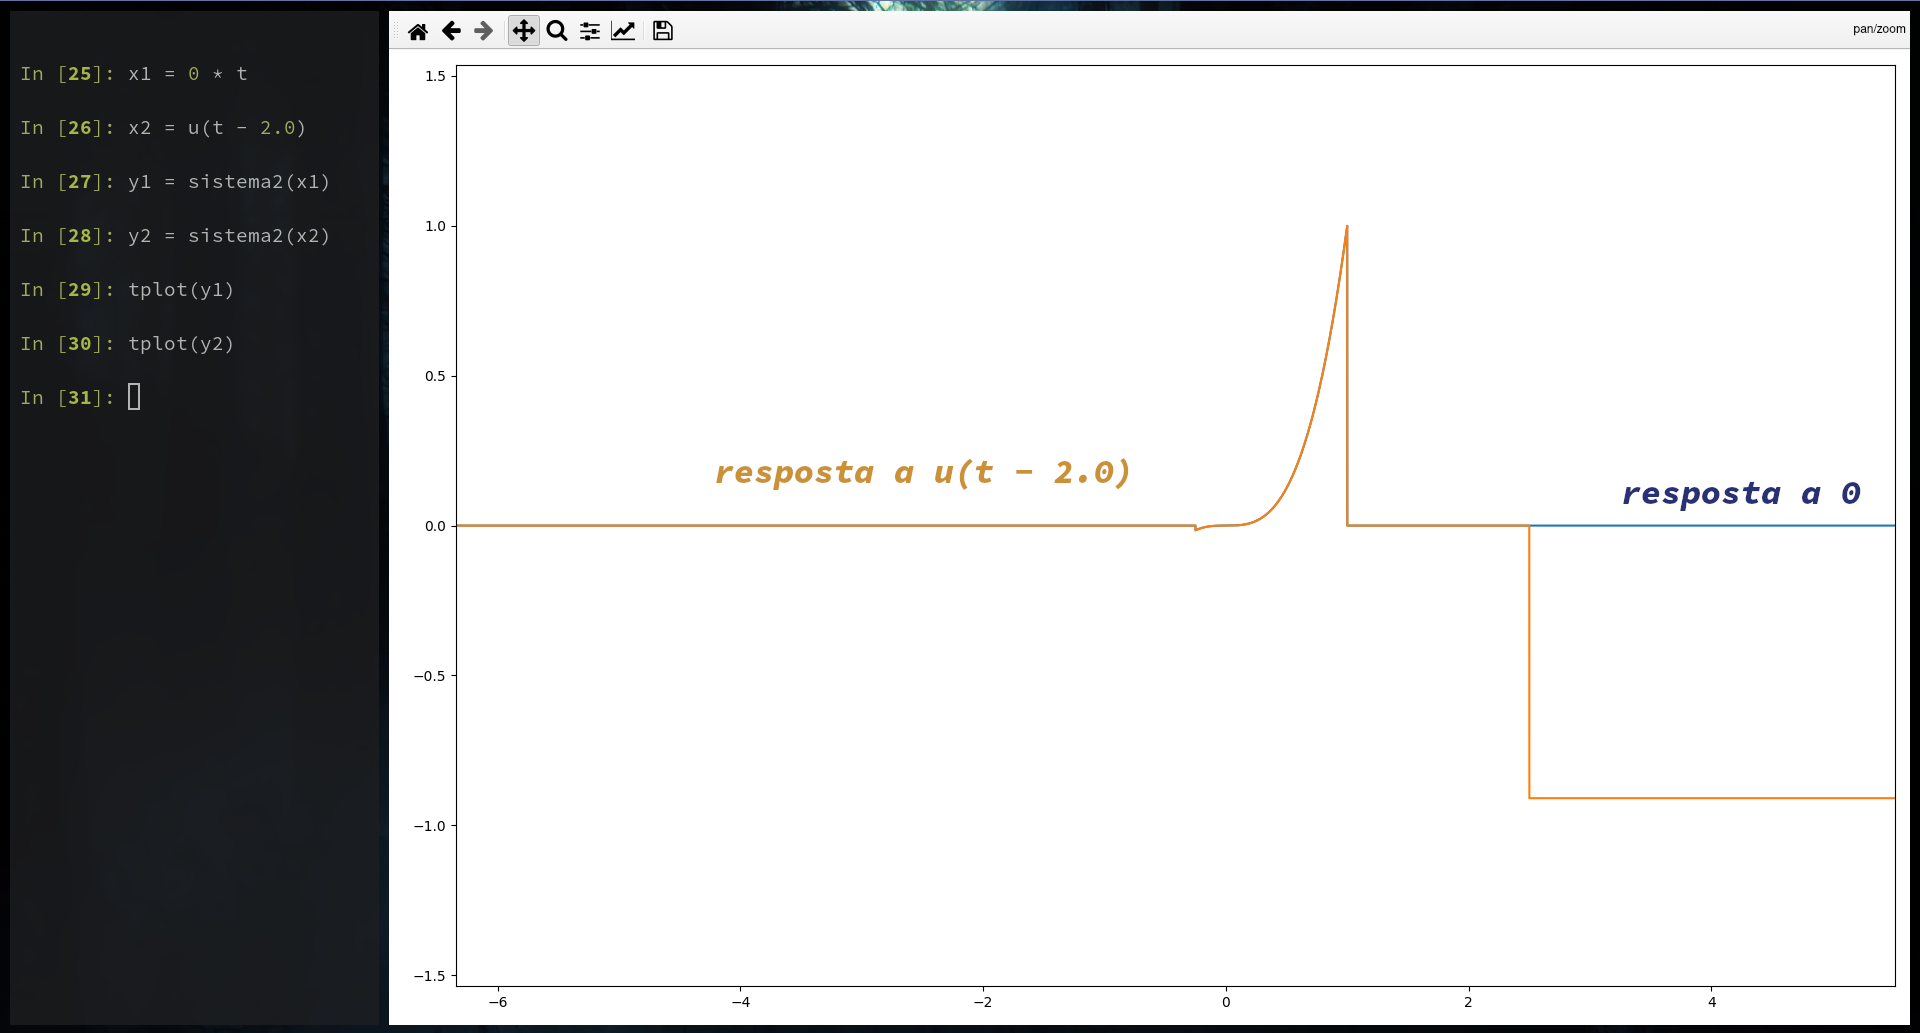
\includegraphics[width = 0.5\linewidth]{prints/causalidade.png}
    \caption{Aparente causalidade, \(sistema_2\).}
    \label{fig:causal}
\end{figure}

Apresentamos então o seguinte exemplo, no qual foram comparadas a resposta do sistema aos sinais de entrada \(x_1(t) = u(t-2)\) e \(x_2(t) \equiv 0\). Ambos os sinas são iguais até ao instante \(t_0=2\) e verifica-se que as saídas também o são.

Após a realização de inúmeros testes\footnotemark[2], no ambito de argumentar a causalidade do \(sistema_2\), foi concluído que \textbf{nada podemos afirmar\footnotemark[3]}, neste aspecto, sobre o sistema. Todos os conjuntos de sinais de entrada testados que de facto, eram iguais até um certo \(t_0\) produziam através do sistema, sinais de saída que aparentavam ser também iguais até ao ponto \(t_0\), pelo que \textbf{o sistema \textit{aparenta} ser causal} (salientamos o facto de não haver certezas absolutas nesta afirmação dado ao método experimental com base na observação direta dos gráficos).
%}}
%------------------------------------------------------%
\subsubsection{(R5) Estabilidade}
\label{subsubsec:R5}
\paragraph{Resposta:} %{{
A \textit{estabilidade} é outra propriedade importante dos sistemas. A resposta de um sistema estável a um sinal de entrada (limitado) resulta num sinal de saída que não diverge, i.e.,
    \[ \text{se}\ x_1(t) \xrightarrow[]{\text{S}} y_1(t)\ \text{e}\ |x_1(t)| \leq A \implies |y_1(t)| \leq B \text{,}\ \text{em que A e B são finitos} \]

Tal como no ponto anterior, a estabilidade é desafiante de abordar apenas por observação das respostas do sistema a sinais de entrada graficamente. Por estes meios, apenas seria possível provar que tal sistema não é estável observando um contra-exemplo.

Foram realizados múltiplos ensaios\footnotemark[2] com variados sinais de entrada limitados com o objetivo de que alguma saída aparentasse não o ser, violando as condições anteriormente enunciadas.

\begin{figure}[ht]
    \centering
    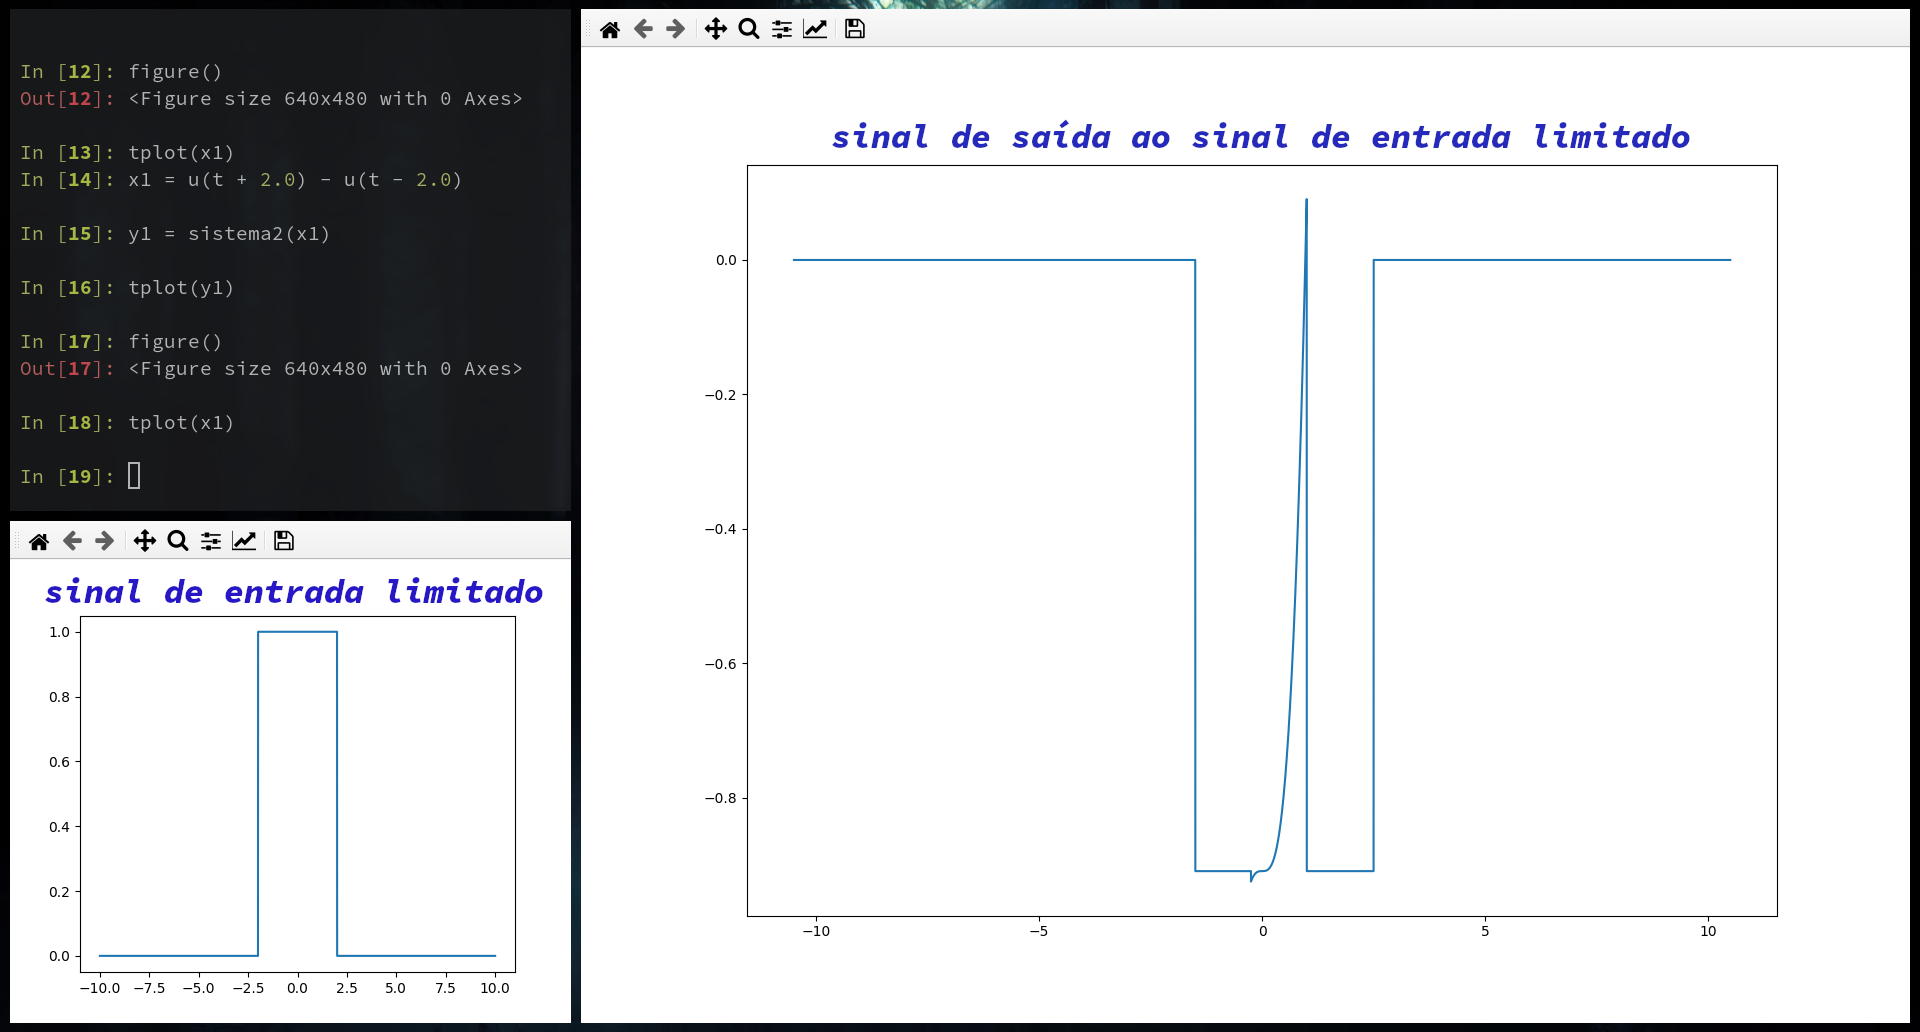
\includegraphics[width = 0.5\linewidth]{prints/estabilidade1.png}
    \caption{Resposta do \(sistema_2\) a um sinal de entrada limitado.}
    \label{fig:estabilidade1}
\end{figure}

Eis um exemplo pertinente na \hyperref[fig:estabilidade1]{Fig. 6}, com \(x(t) = u(t+2) - u(t-2)\), note-se que o sinal de entrada \(x(t)\) é limitado e a sua saída também o é.

Foi concluído que \textbf{nada podemos afirmar}\footnotemark[3], nas condições da propriedade enunciada, sobre a estabilidade do nosso sistema desconhecido, \(sistema_2\). Pelo que apenas podemos referir que o nosso \textbf{sistema \textit{aparenta} ser estável}.

\footnotetext[2]{De modo a manter a discussão concisa, alguns dos resultados brutos podem ser encontrados no apêndice.}

\footnotetext[3]{É necessário realçar com bastante importância que uma análise gráfica não nos permitirá ter a certeza sobre uma dada propriedade na maioria dos casos razoáveis, a não ser, claro, que seja visualizado um contra-exemplo que demonstre que a propriedade enunciada \textbf{não} se verifica!}

\clearpage

\subsection{\bf{Resposta em frequência}}
\label{subsec:respostafreq}
%------------------------------------------------------%
\subsubsection{(R6) Circuito RC}
\label{subsubsec:R6}
\textbf{Sabendo que C = \(500 \mu F\), estime, justificadamente, o valor da resistência \(R\), usando os resultados experimentais que obteve. Descreva como se certificou de que o valor estimado para \(R\) está de acordo com os resultados experimentais respeitantes a ambos \(\mathcal{H}(j \omega)\) e \(h(t)\).}

\paragraph{Resposta:} %{{
O circuito RC apresentado é um exemplo clássico de um SLIT, i.e., pode ser visto como a relação: \(x(t) * h(t) = y (t) \iff x(t) \xrightarrow[]{\text{S}} y(t)\).

Deste modo, é trivial deduzir a expressão analítica de \(h(t)\) para este sistema com os conhecimentos adquiridos. 

De modo a manter o relatório sintético, e dado que escapa ao âmbito da questão, não incluímos a dedução das seguintes expressões analíticas\footnotemark[4]:

$$ h(t) = \frac{1}{RC}e^{\frac{-t}{RC}} \cdot u(t) $$

$$ \mathcal{H}(j\omega) = \frac{1}{1 + j\omega RC} $$

Obtidas as expressões que caracterizam o \(sistema_3\) procedemos à análise experimental para estimar o valor da resistência \(R\) que respeita as condições do enunciado.

\footnotetext[4]{No entanto, estas podem ser encontradas no apêndice, para um leitor interessado.}

\begin{normalsize}
\vspace{0.5cm}
\underline{1. Observação direta de \(h(t)\)} 
\vspace{0.25cm}
\end{normalsize}

Fazendo \(\delta(t)\) o sinal de entrada do \(sistema_3\), temos que a saída será \(h(t)\), por definição.

Dada a expressão de \(h(t)\) é imediato verificar que quando \(t = 0\) encontramo-nos no seu máximo, que corresponde a \(\frac{1}{RC}\). Para se obter \(R\), é uma questão de manipulações algébricas dado que conseguimos obter \(h(0)\) através do máximo do gráfico de \(h(t) = y(t) = sistema_{3}(\delta(t))\).

\begin{figure}[H]
    \centering
    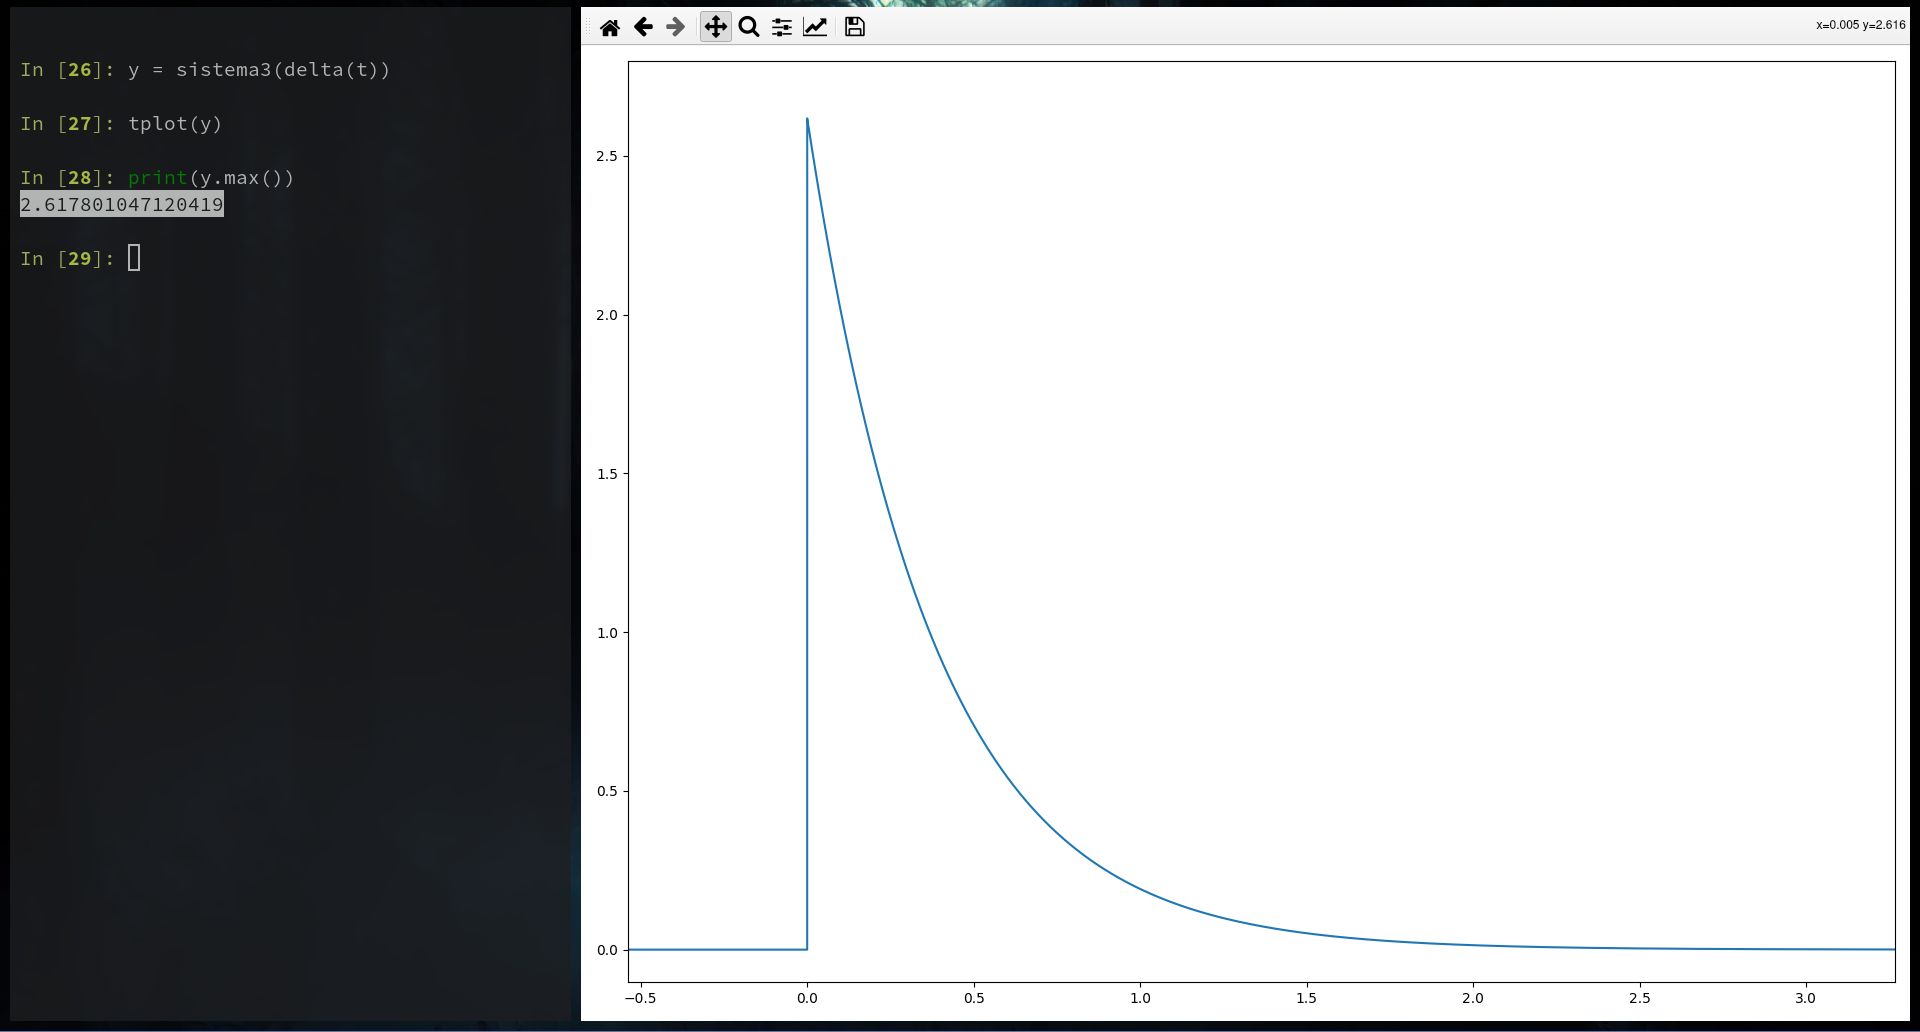
\includegraphics[width = 0.5\linewidth]{prints/ht.png}
    \caption{Valor experimental de \(h(0)\).}
    \label{fig:ht}
\end{figure}

\[h(0) = \frac{1}{RC} \approx 2.6178 \implies R \approx \frac{1}{C \cdot h(0)} \approx 764.0\ \Omega \]

\clearpage

\begin{normalsize}
%\vspace{0.5cm}
\underline{2. Observação de \(\mathcal{H}(j\omega)\)}
\vspace{0.25cm}
\end{normalsize}

No intuito de simplificar cálculos e visualizar a função de transferência diretamente no ambiente laboratorial com base em \textit{Python}, foi necessário tomar o valor absoluto de \(\mathcal{H}(j\omega)\).

É facilmente deduzido que, 
\[\vert \mathcal{H}(j\omega)\vert = \frac{1}{\sqrt{1 + (\omega RC)^2}}\text{, pelo que, quando }\omega = \frac{1}{RC} \implies \vert \mathcal{H}(j\frac{1}{RC})\vert = \frac{\sqrt{2}}{2}\]

Nesta configuração, o seguinte passo foi analisar o gráfico de \(\vert \mathcal{H}(j\omega)\vert\) e descobrir experimentalmente a abcissa (em \(\frac{1}{RC}\)) que corresponde ao valor de \(\frac{\sqrt{2}}{2}\) no eixo das ordenadas.

\begin{figure}[H]
    \centering
    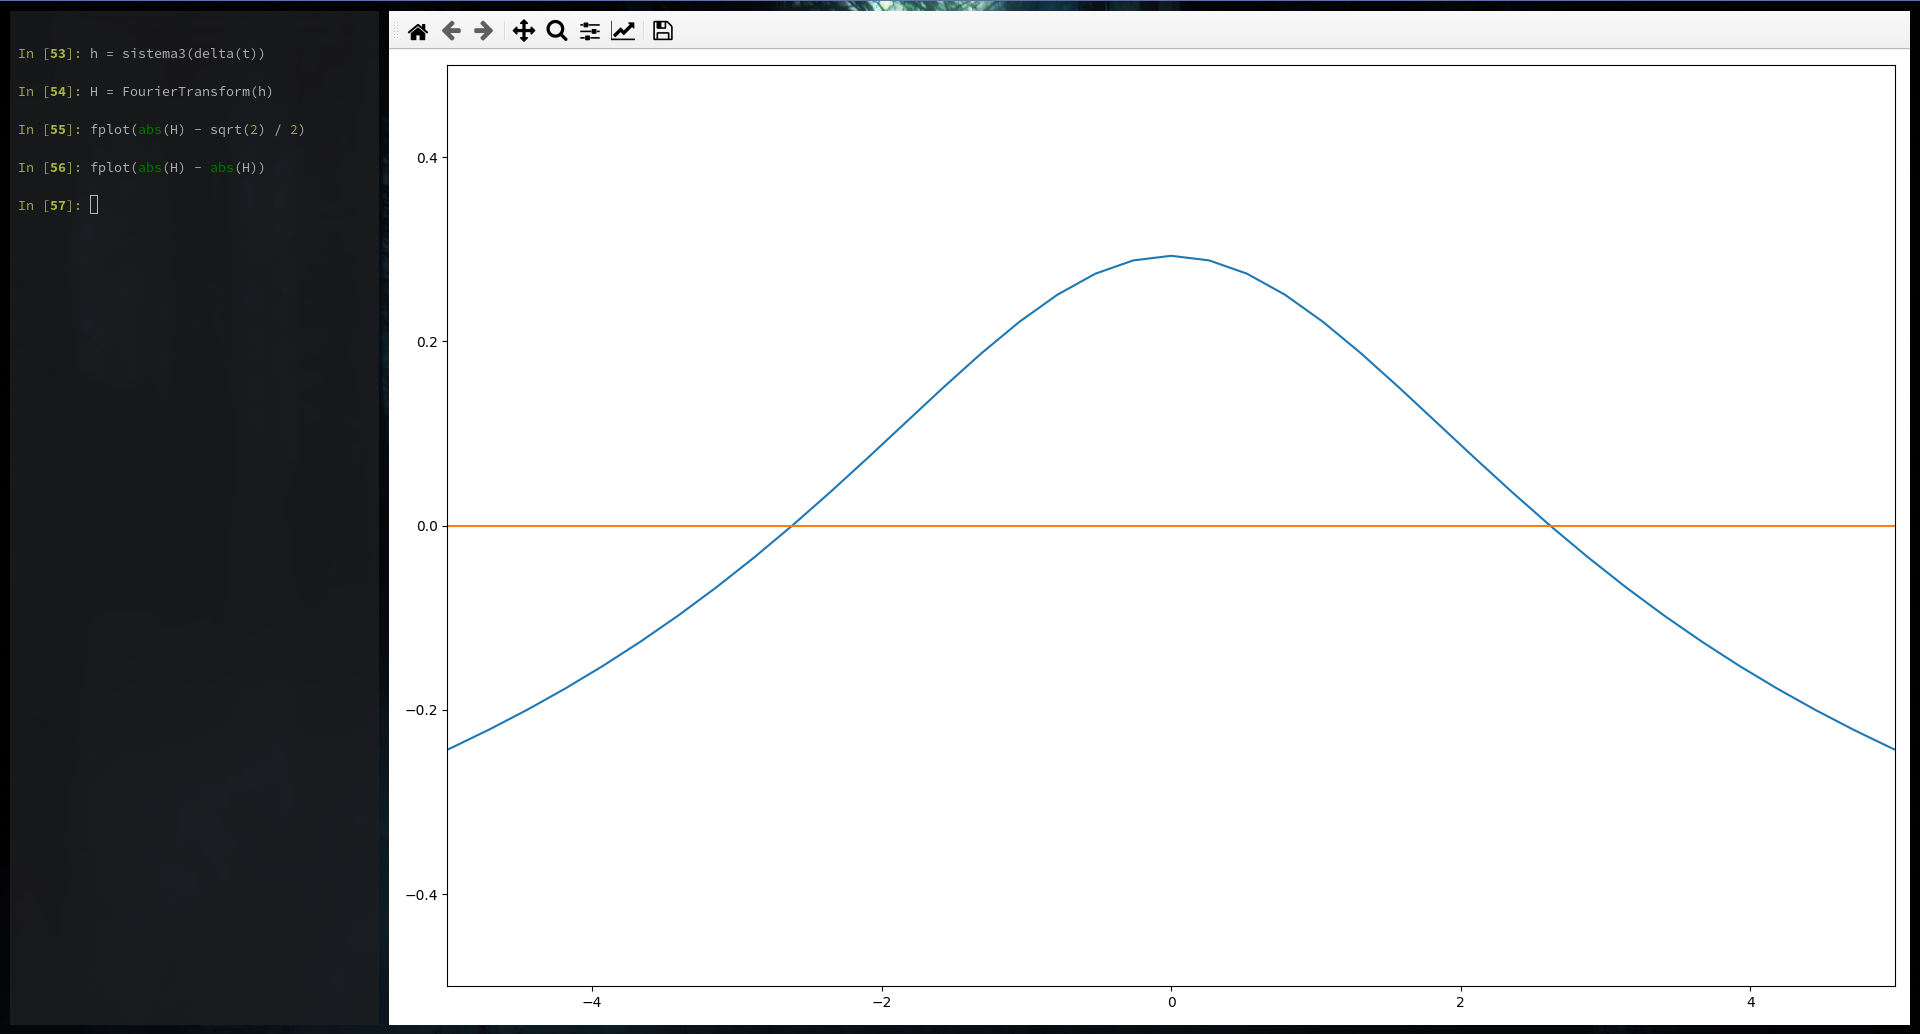
\includegraphics[width = 0.5\linewidth]{prints/transf_ht.png}
    \caption{Valor experimental de \(\frac{1}{RC}\).}
    \label{fig:transf_ht}
\end{figure}

A \hyperref[fig:transf_ht]{Fig. 8} contempla a interseção de \(\vert \mathcal{H}(j\omega)\vert \) deslocado no eixo das ordenadas \(\frac{\sqrt{2}}{2}\) com a reta auxiliar \(y(\omega) \equiv 0\), para uma visualização mais precisa. Deste modo, foi obtido um valor no eixo das abcissas \(x_{exp} \approx 2.6180\).

\[x_{exp} = \frac{1}{RC} \approx 2.6180 \implies R \approx \frac{1}{x_{exp} \cdot C} \approx 763.9\ \Omega\]

\clearpage 

Deste modo, \textbf{concluímos que \(R \approx 764\ \Omega\)} com base nos resultados das duas experiências\footnotemark[5]. Em seguida realizamos a sobreposição do \(h(t)\) produzido como saída do \(sistema_3\) com \(h_{exp}(t)\) que nada mais é do que a representação da expressão analítica anteriormente deduzida, com \(R = 764\ \Omega\). Foi realizado, analogamente, um teste para \(\vert \mathcal{H}(j\omega)\vert \), com o respetivo \(\vert \mathcal{H}_{exp}(j\omega)\vert \).

Observou-se um resultado bastante satisfatório para \(R\) obtido experimentalmente, visto que respeita \(\mathcal{H}(j\omega)\) e \(h(t)\), como é explícito nas seguintes \hyperref[fig:multiplas_2]{Fig. 9} e \hyperref[fig:multiplas_3]{Fig. 10}.

\begin{figure}[H] 
    \begin{subfigure}[b]{0.5\linewidth}
        \centering
        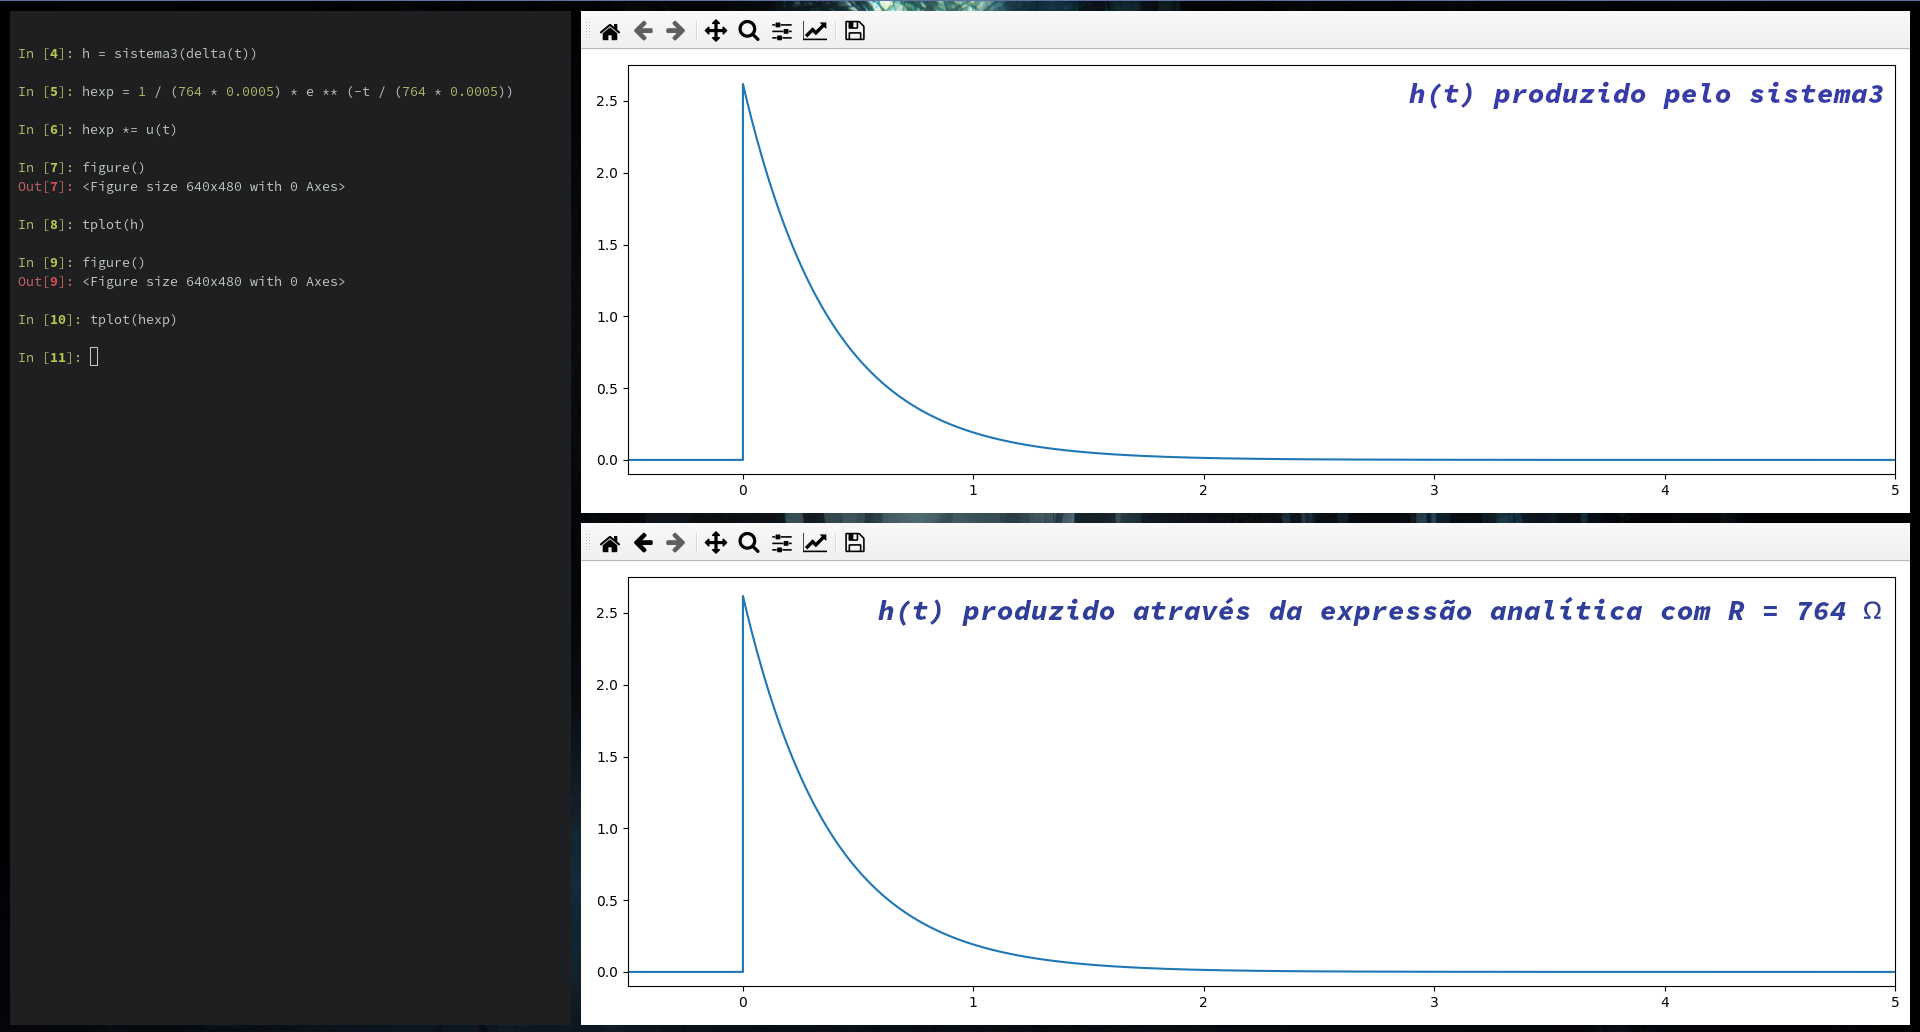
\includegraphics[width=1\linewidth]{prints/ht_exp_lado_a_lado.png}
        \caption{\(h(t)\ \text{e}\ h_{exp}(t)\).} 
        \label{fig:ht_exp_lado_a_lado} 
        %%\vspace{4ex}
    \end{subfigure}%% 
    \begin{subfigure}[b]{0.5\linewidth}
        \centering
        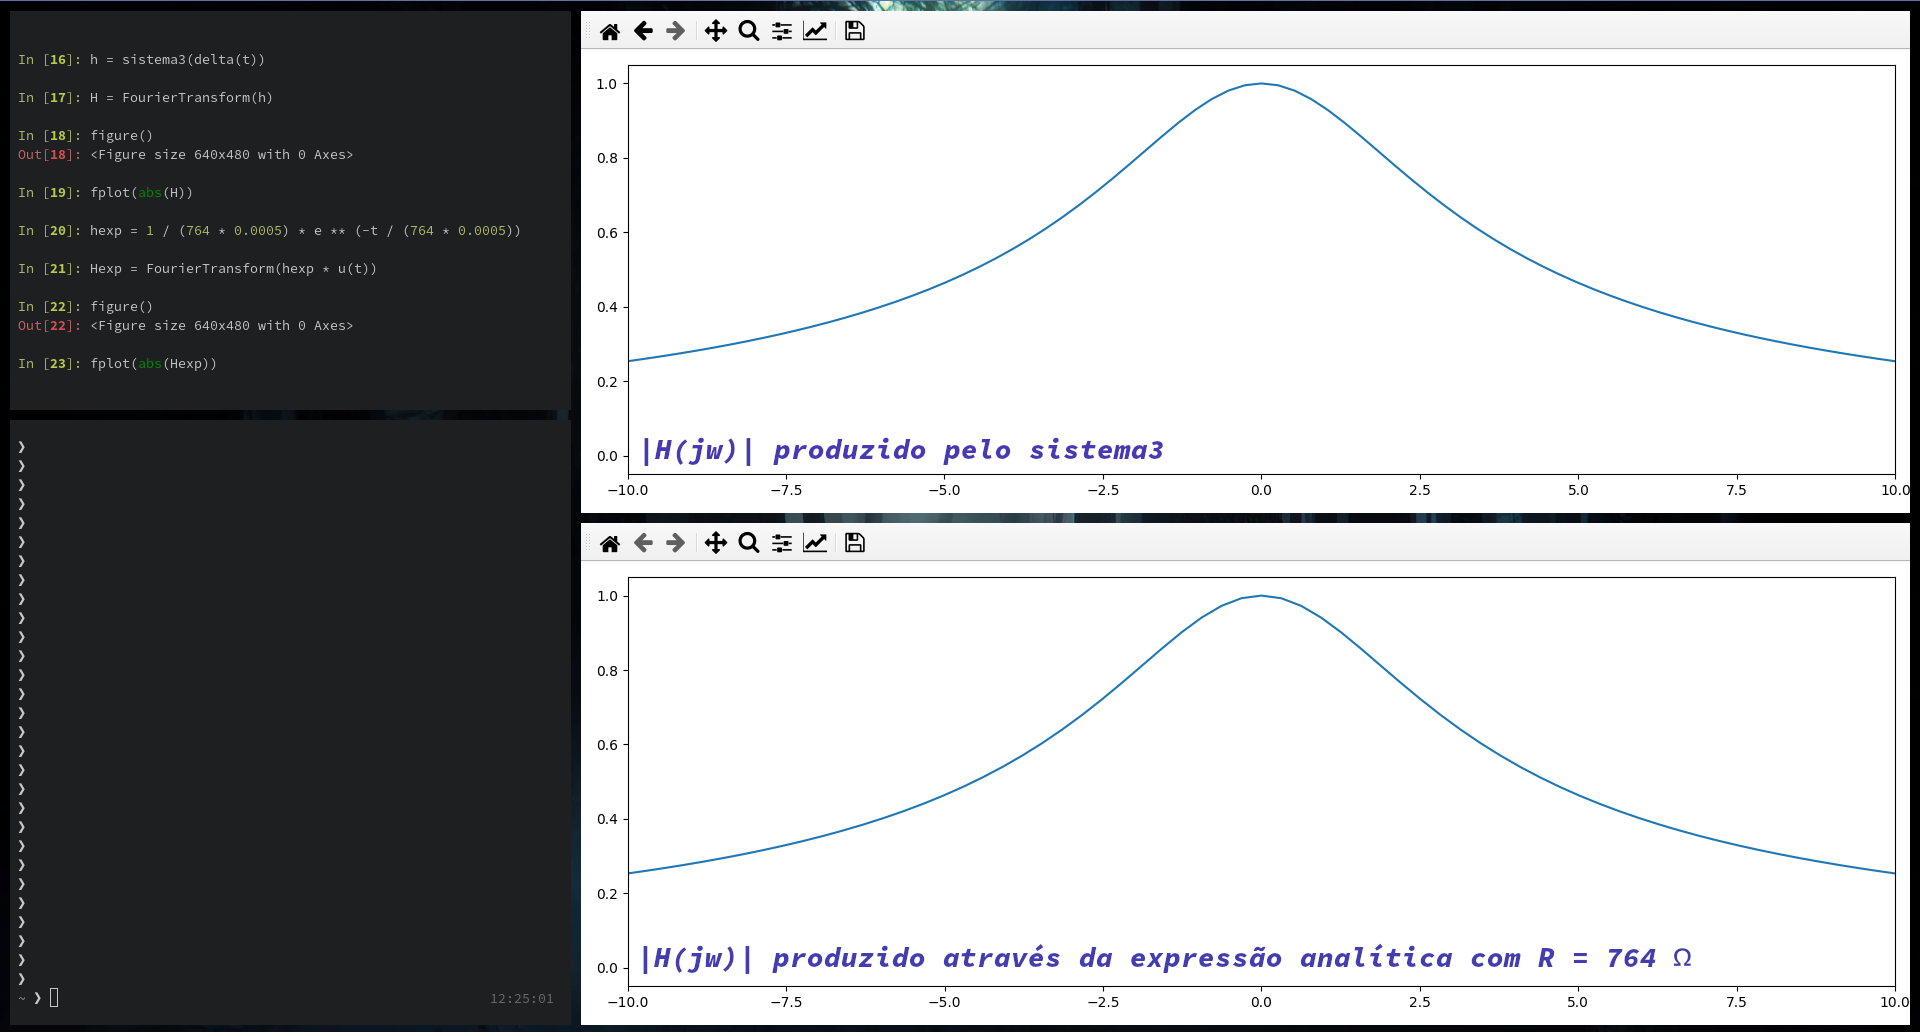
\includegraphics[width=1\linewidth]{prints/transf_ht_exp_lado_a_lado.png} 
        \caption{\(\vert \mathcal{H}(j\omega)\vert \ \text{e}\ \vert \mathcal{H}_{exp}(j\omega)\vert\).} 
        \label{fig:transf_ht_exp_lado_a_lado} 
        %%\vspace{4ex}
    \end{subfigure} 
    \caption{Comparação lado a lado dos resultados obtidos.}
    \label{fig:multiplas_2}
\end{figure}

\begin{figure}[H] 
    \begin{subfigure}[b]{0.5\linewidth}
        \centering
        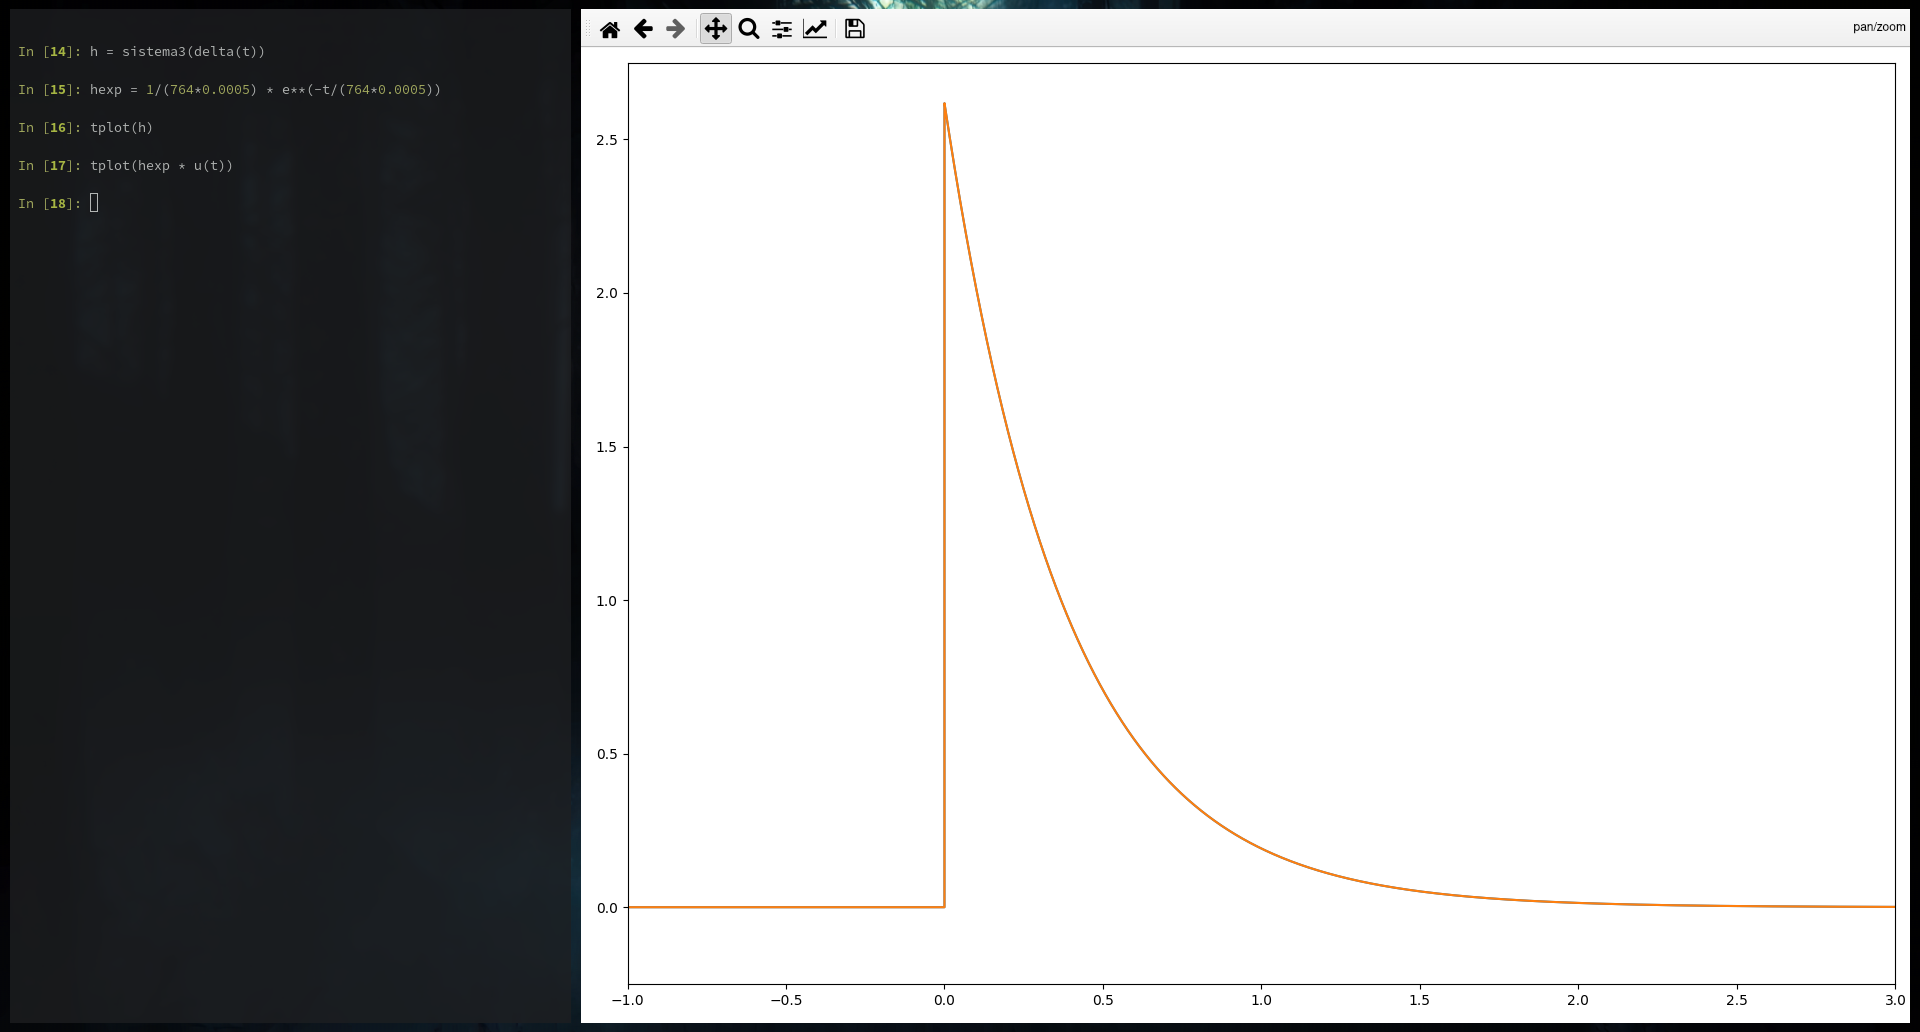
\includegraphics[width=1\linewidth]{prints/ht_exp.png}
        \caption{Sobreposição de \(h(t)\ \text{e}\ h_{exp}(t)\).} 
        \label{fig:ht_exp} 
        %%\vspace{4ex}
    \end{subfigure}%% 
    \begin{subfigure}[b]{0.5\linewidth}
        \centering
        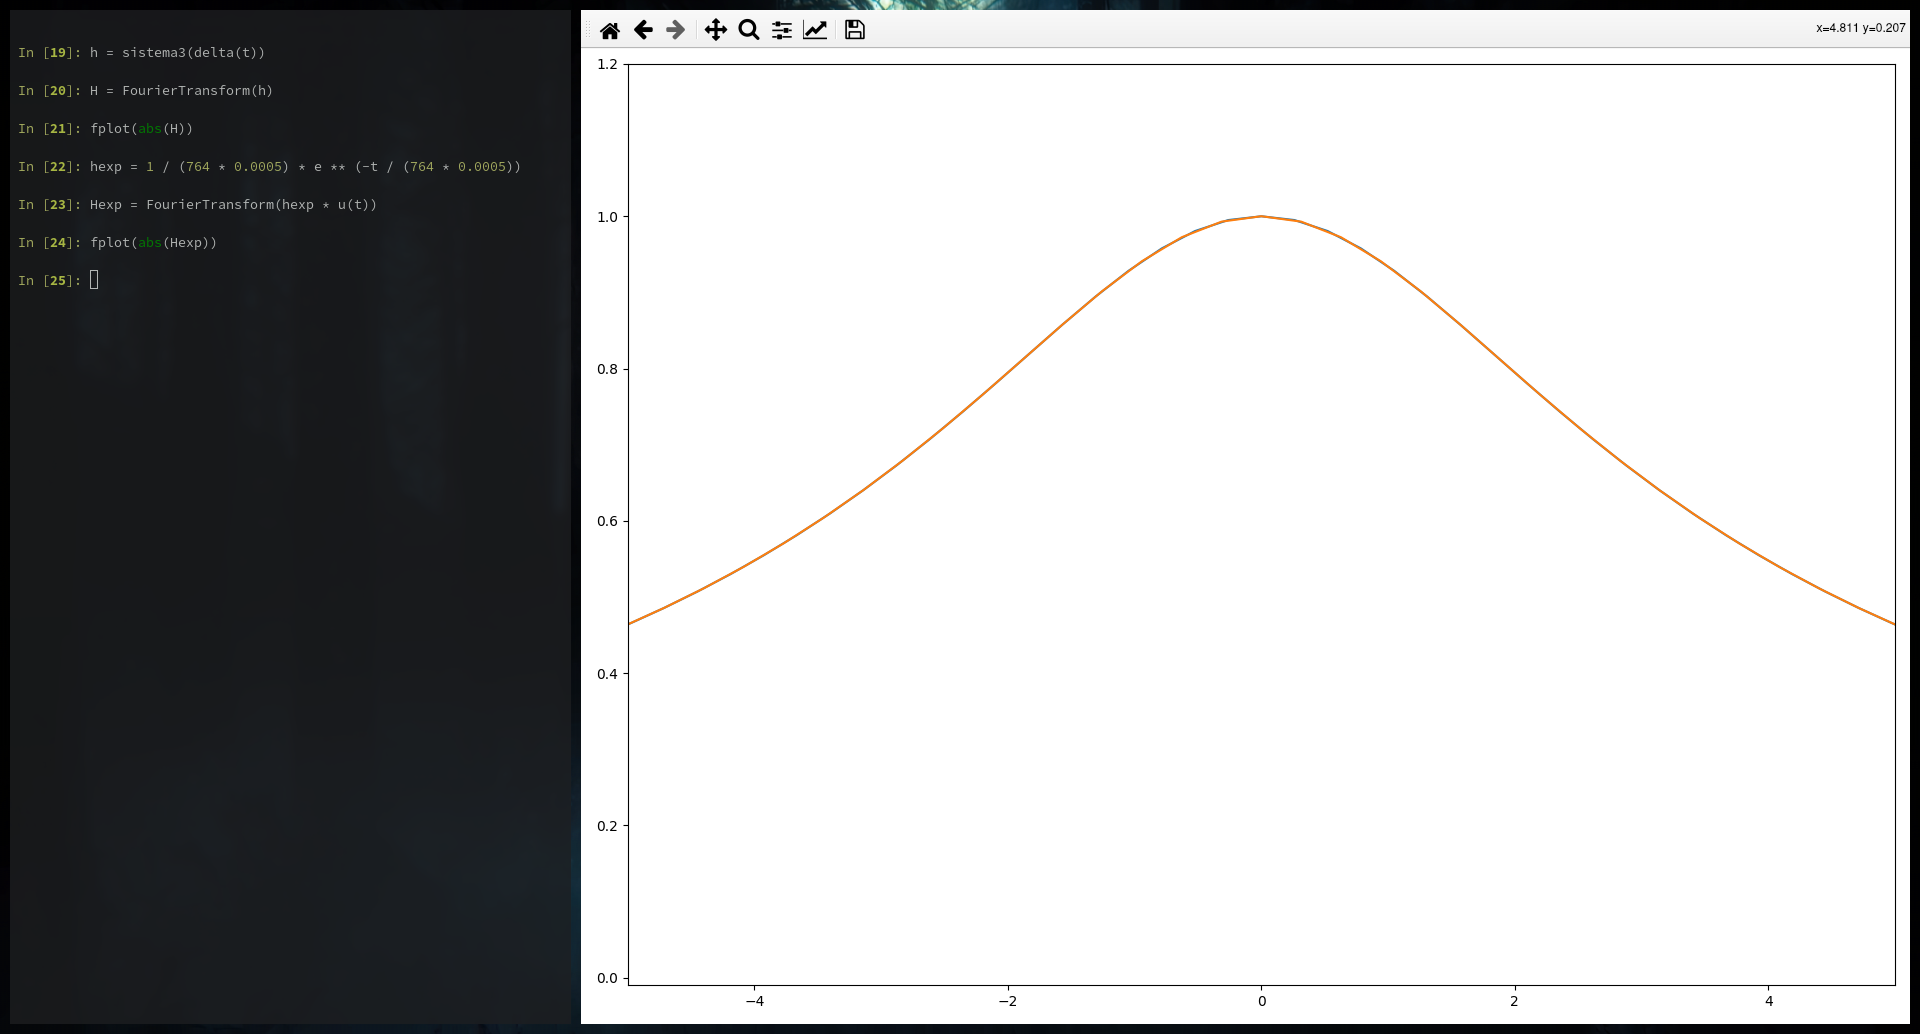
\includegraphics[width=1\linewidth]{prints/transf_ht_exp.png} 
        \caption{Sobreposição de \(\vert \mathcal{H}(j\omega)\vert \ \text{e}\ \vert \mathcal{H}_{exp}(j\omega)\vert\).} 
        \label{fig:transf_ht_exp} 
        %%\vspace{4ex}
    \end{subfigure} 
    \caption{Comparação por sobreposição dos resultados obtidos.}
    \label{fig:multiplas_3}
\end{figure}

Note-se que na \hyperref[fig:multiplas_3]{Fig. 10} os gráficos estão sobrepostos de modo a uma comparação mais refinada dos resultados obtidos.

\footnotetext[5]{É se salientar que estamos cientes das possíveis diferenças inobserváveis a olho nu entre os pares de gráficos.  Existem sempre incertezas derivadas de medições por observação (erro humano), e claro, limitações que as operações em números em vírgula flutuante acartam.}

\clearpage
\subsection{\bf{Filtragem}}
\label{subsec:filtragem}
%------------------------------------------------------%
\subsubsection{(R7) Passa-baixo e passa-alto}
\label{subsubsec:R7}
\textbf{A saída do filtro passa-baixo reproduz bem as zonas de variação rápida do sinal \(p\)? E as de variação lenta? E do passa-alto? Explique porquê.}
\paragraph{Resposta:} %{{
O filtro \underline{passa-baixo} não ideal modelado no sistema laboratorial em \textit{Python} (\(sistema_4\)) prevê uma frequência de corte \(\vert f_{c}\vert = 500\ Hz\). 

Como é possível observar na \hyperref[fig:ganho_passa-baixo]{Fig. 11}, \(\vert \mathcal{H}_4(j\omega)\vert\) atenua bastante as altas frequências \(\vert f\vert > 500\ Hz\) (i.e., as zonas de variação rápida) de um sinal de entrada. O que seria de esperar uma vez que a saída, em frequência, é dada por \(\mathcal{Y}(j\omega) = \mathcal{H}(j\omega) \cdot \mathcal{P}(j\omega)\).

\begin{figure}[H]
    \centering
    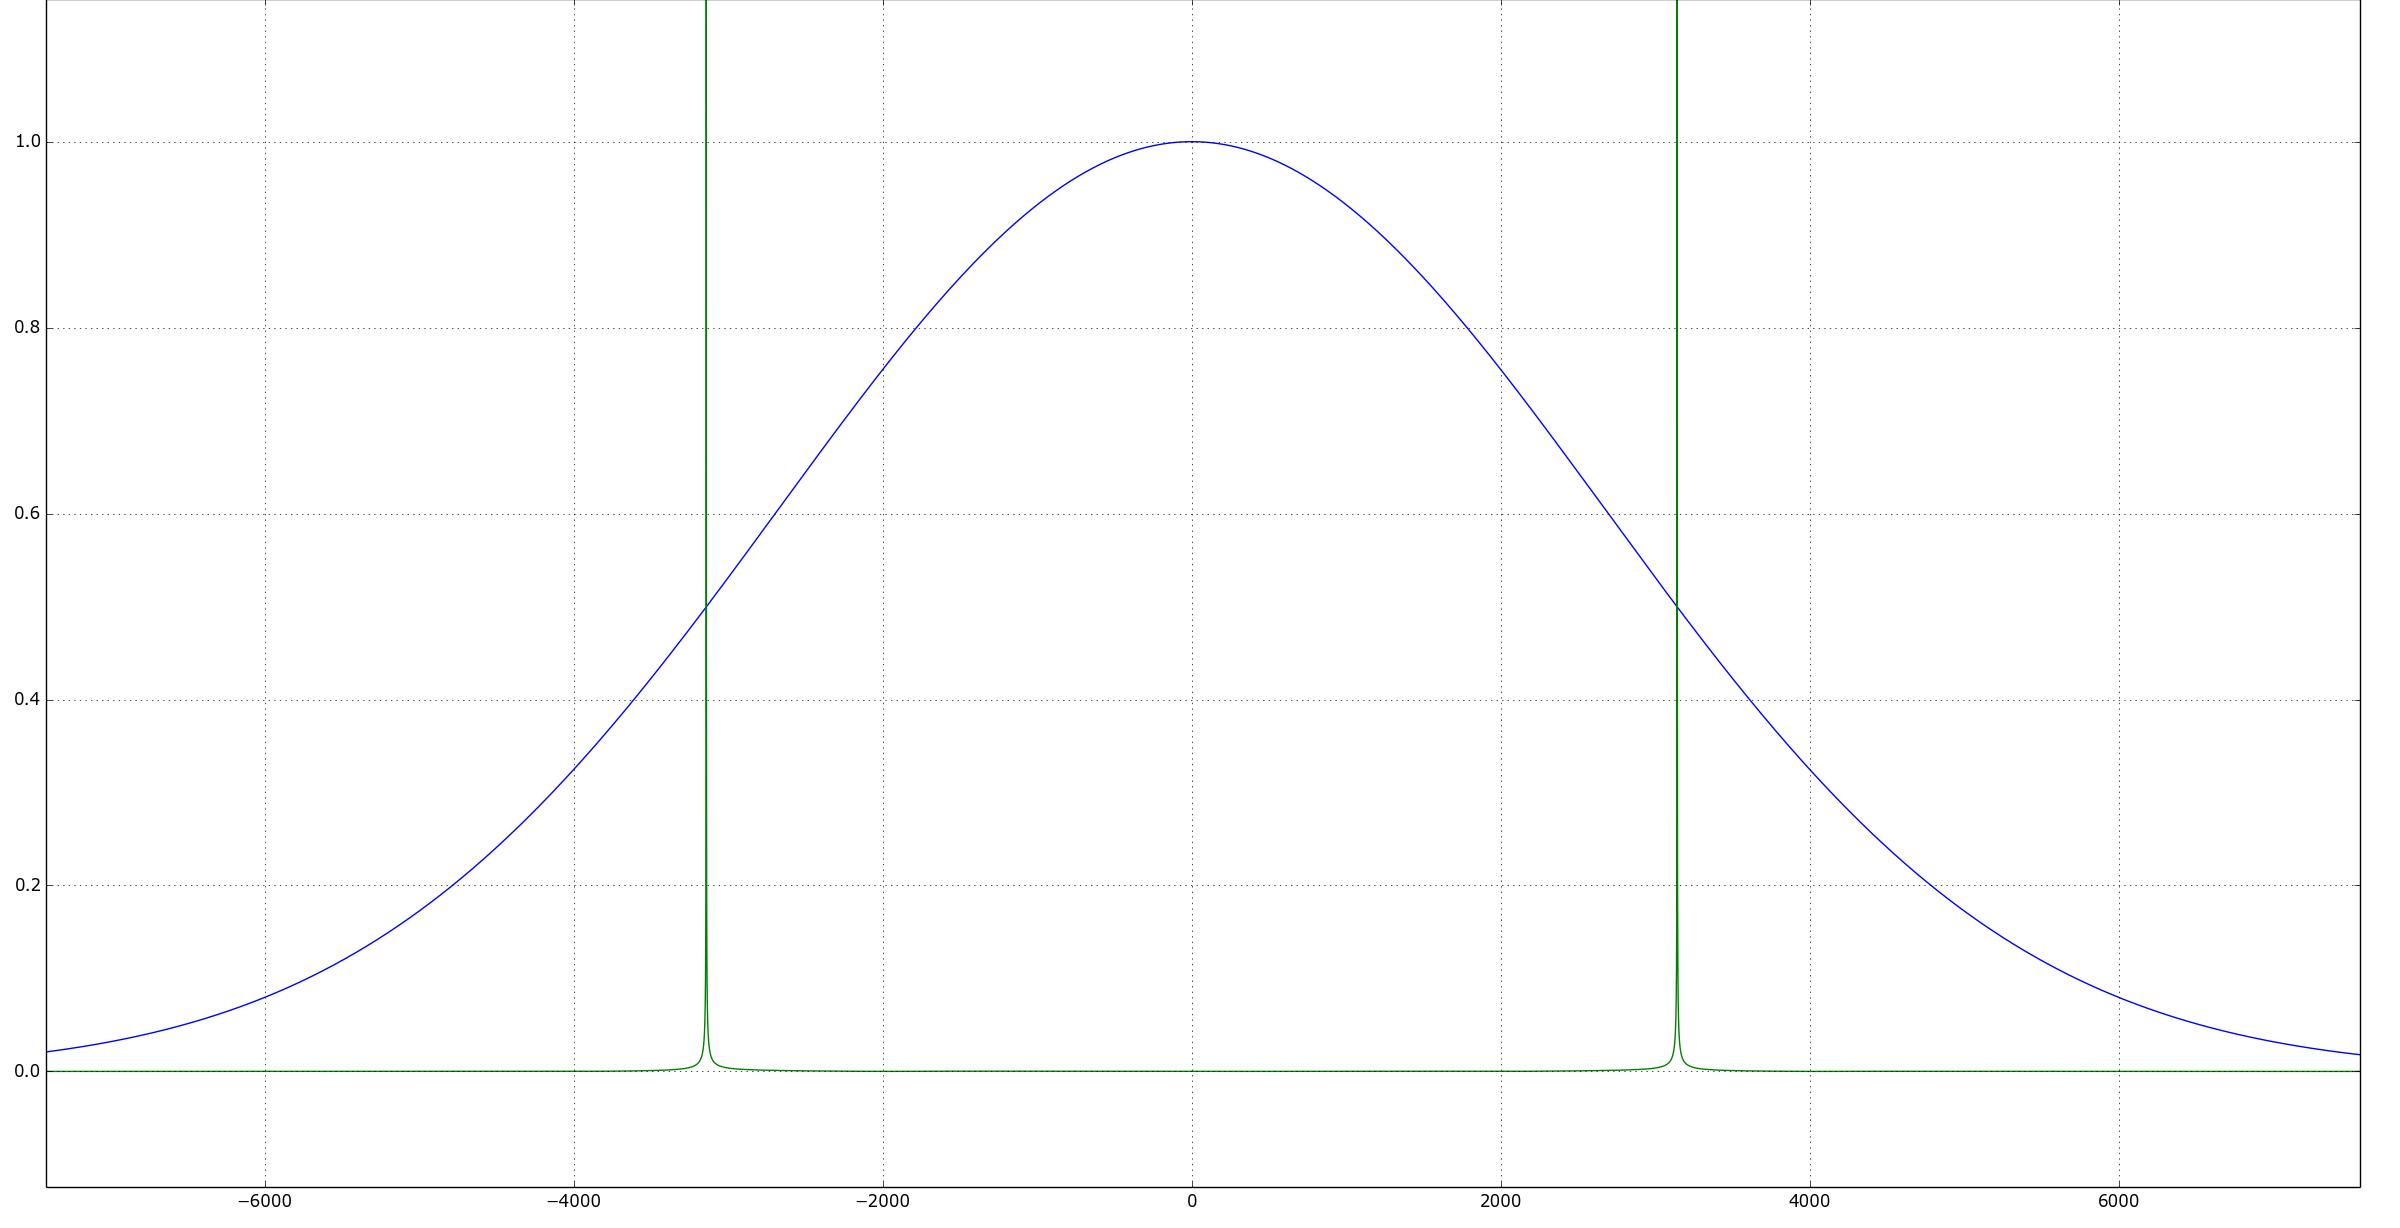
\includegraphics[width = 0.5\linewidth]{prints/ganho_passa-baixo.png}   
    \caption{\(\vert \mathcal{H}_4(j\omega)\vert\) com \(\vert \omega_{c}\vert = 2\pi \cdot \vert f_{c}\vert = 1000\pi\ \text{rad}\ s^{-1}\).}
    \label{fig:ganho_passa-baixo}
\end{figure}

\begin{figure}[ht] 
    \begin{subfigure}[b]{0.5\linewidth}
        \centering
        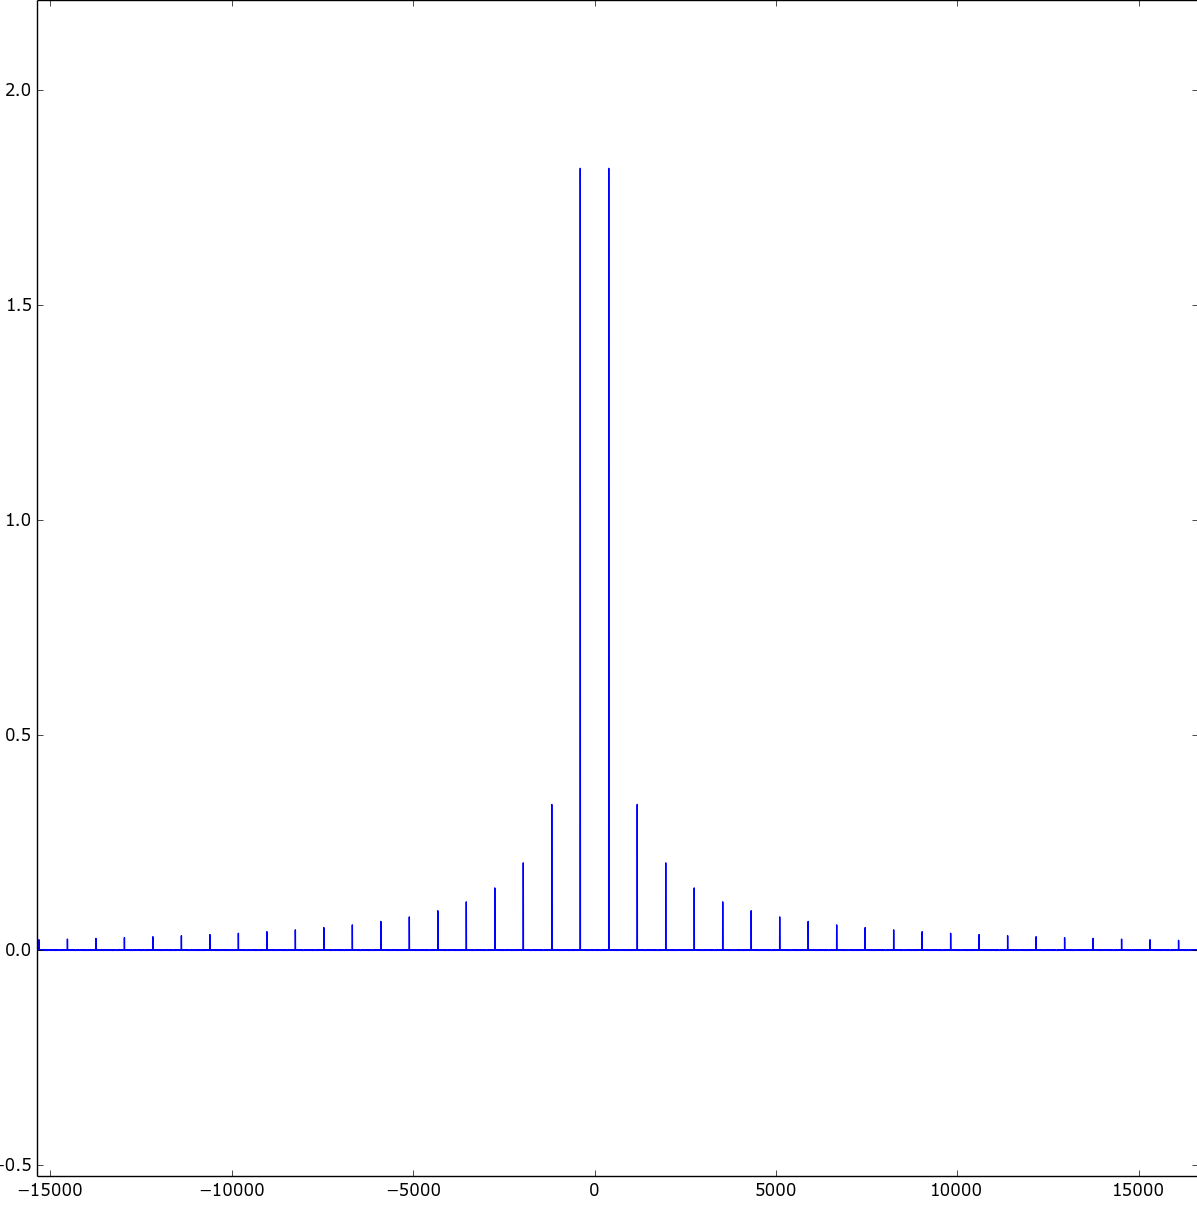
\includegraphics[width=1\linewidth]{prints/p_normal.png}
        \caption{Sinal \(p\) original.} 
        \label{fig:p_normal} 
        %%\vspace{4ex}
    \end{subfigure}%% 
    \begin{subfigure}[b]{0.5\linewidth}
        \centering
        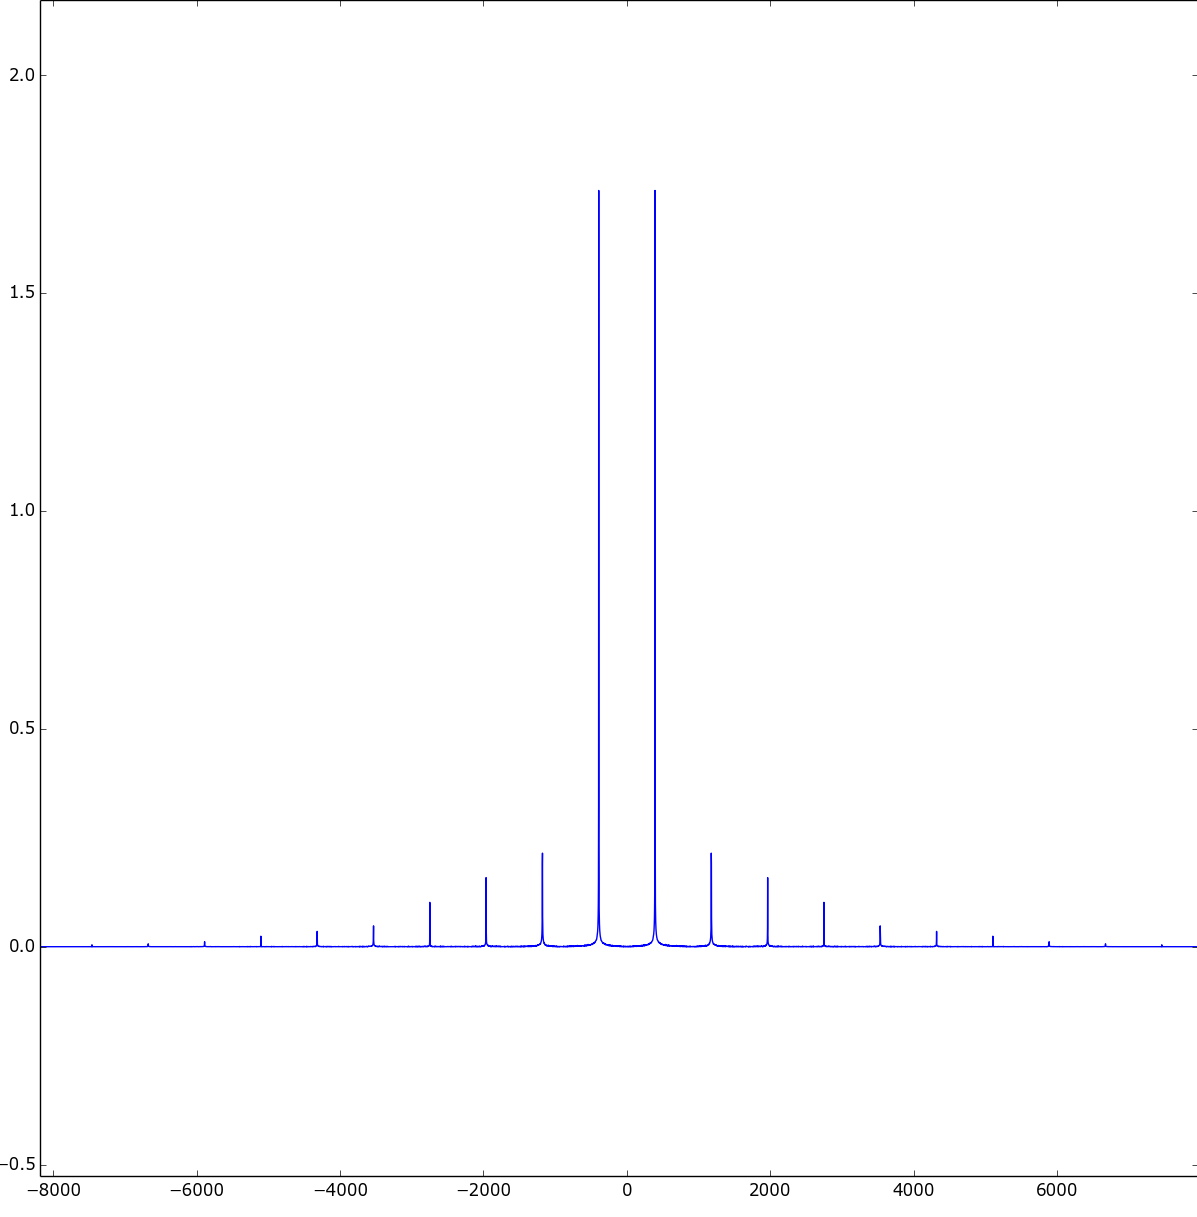
\includegraphics[width=1\linewidth]{prints/p_atenuado.png} 
        \caption{Sinal \(p\) atenuado pelo filtro passa-baixo.} 
        \label{fig:p_atenuado} 
        %%\vspace{4ex}
    \end{subfigure} 
    \caption{Comparação entre a resposta em frequência (angular, \(\omega = 2\pi f\)) do sinal \(p\) original e do sinal \(p\) atenuado pelo filtro passa-baixo. (Note-se a escala diferente).}
    \label{fig:multiplas_4}
\end{figure}

O oposto é visualizado nas zonas de baixas frequências \(\vert f\vert < 500\ Hz\) (variação lenta) em que o ganho tende para \(1\) quando a frequência \(f\) tende para \(0\ Hz\), i.e., em termos práticos serão estas frequências que melhor se reproduzem do sinal \(p\). O filtro passa-baixo, reproduz melhor as zonas de variação rápida do sinal \(p\).

\clearpage

No caso, do filtro \underline{passa-alto} não ideal (\(sistema_5\)) é intuitivo perceber que o oposto do discutido sobre o filtro anterior ocorrerá. Isto é, as zonas de variação alta serão bem reproduzidas, enquanto as zonas de variação lenta serão bastante atenuadas como é evidente após observação direta do modulo da função de transferência deste sistema na \hyperref[fig:ganho_passa-alto]{Fig. 13}.

%\iffalse
\begin{figure}[H]
    \centering
    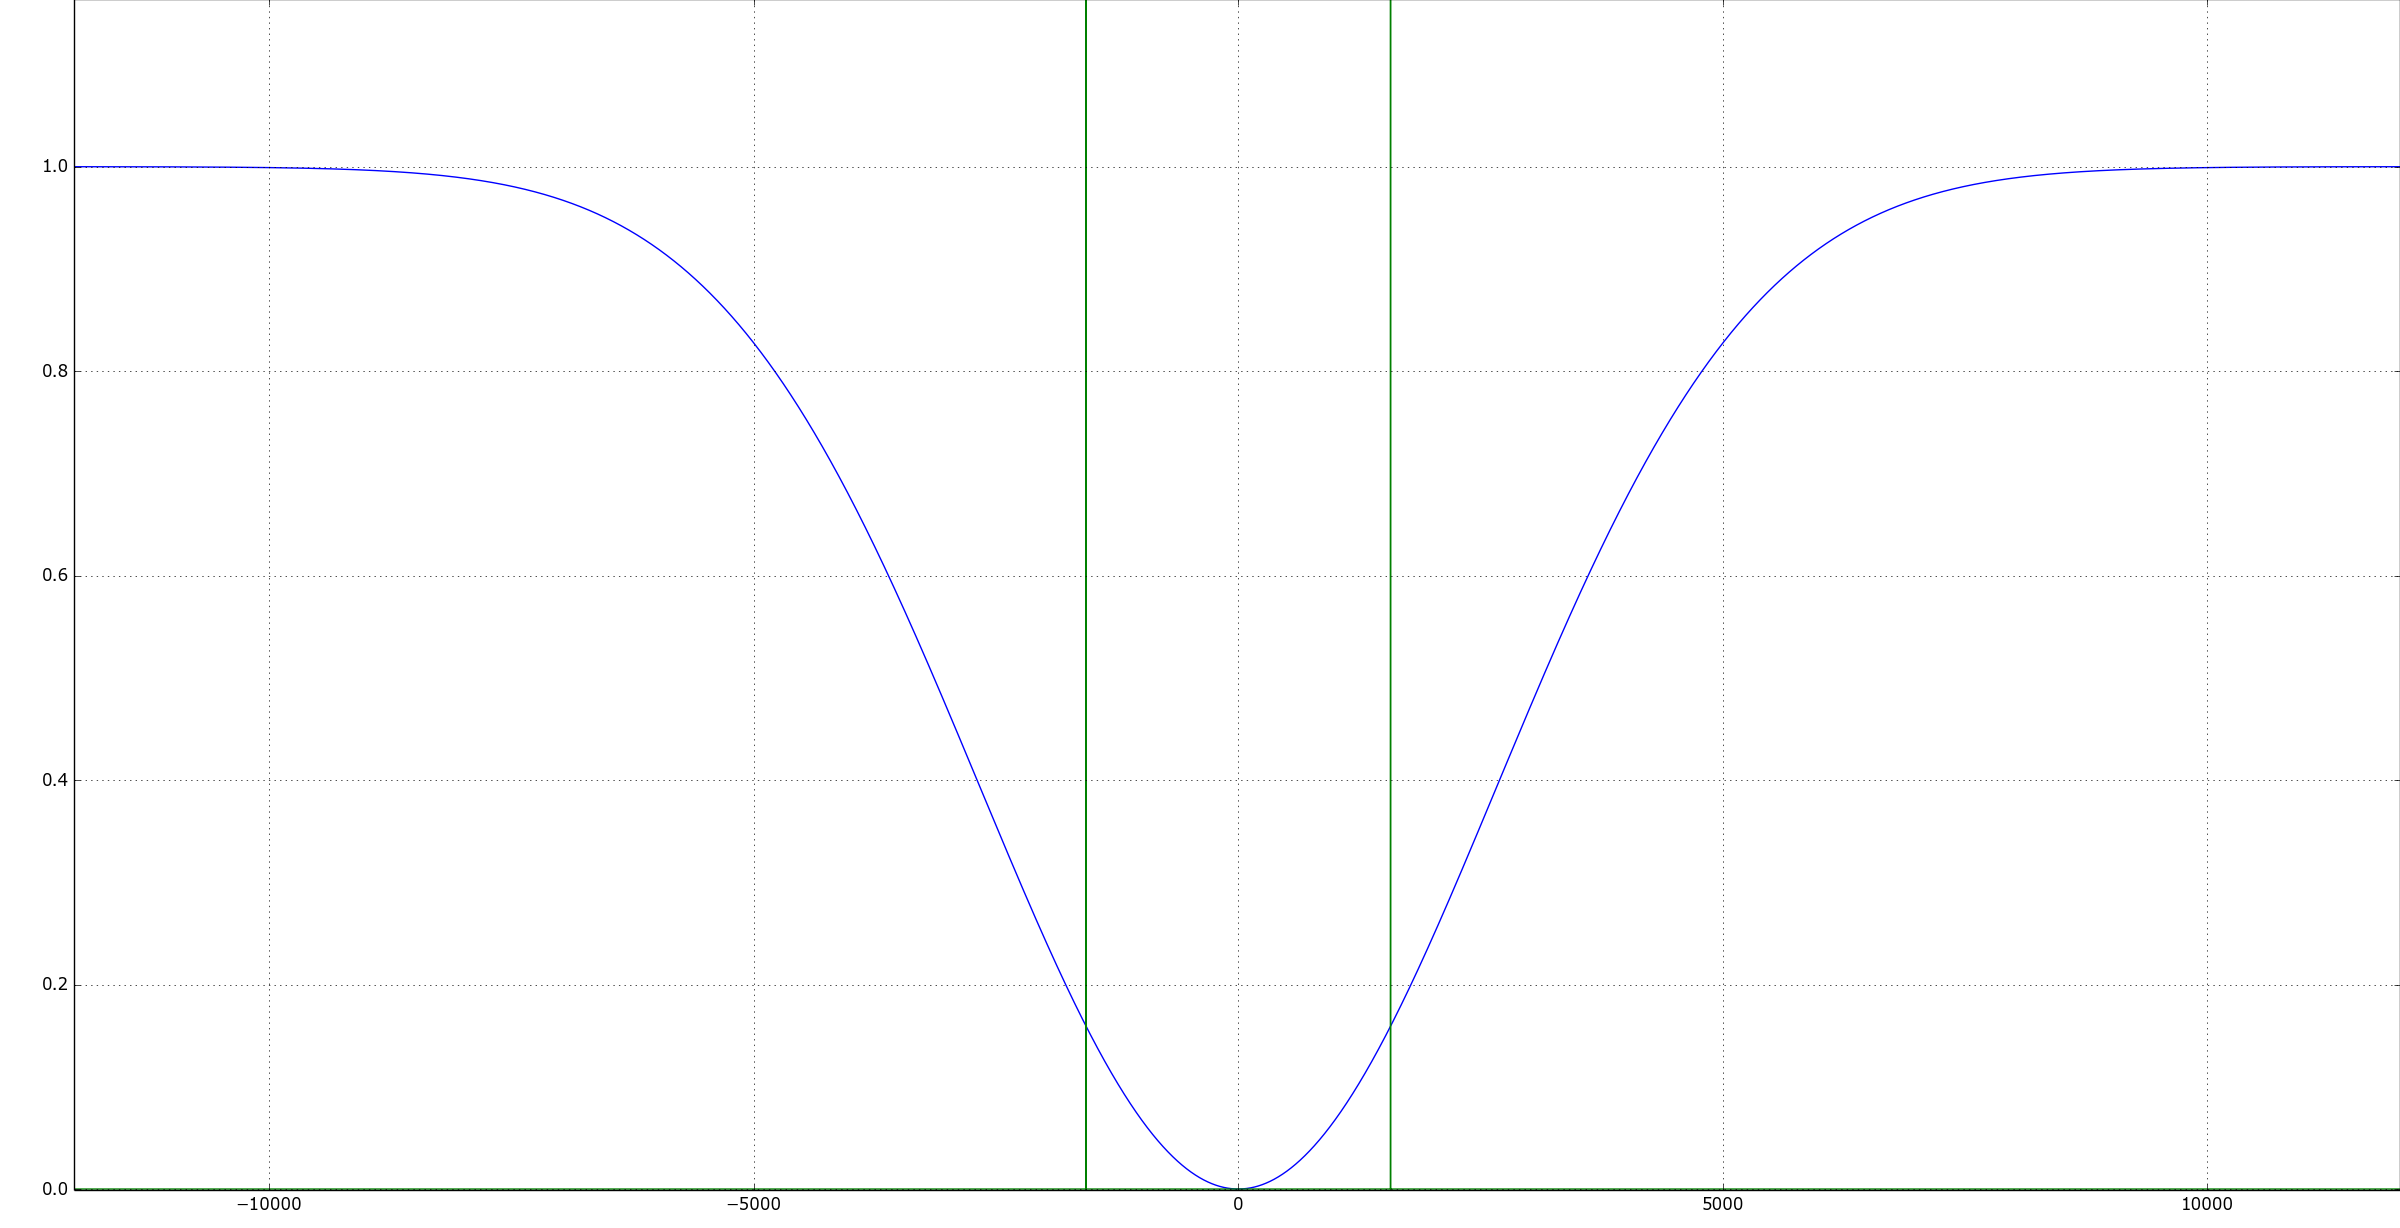
\includegraphics[width = 0.5\linewidth]{prints/ganho_passa-alto.png}   
    \caption{\(\vert \mathcal{H}_5(j\omega)\vert\) com \(\vert \omega_{c}\vert = 2\pi \cdot \vert f_{c}\vert = 500\pi\ \text{rad}\ s^{-1}\).}
    \label{fig:ganho_passa-alto}
\end{figure}
%\fi

É possível concluir que para as frequências \(\vert f \vert\) acima da \(\vert f_c \vert = 250\ Hz\), o ganho tende para \(1\), enquanto para frequências mais baixas, o sinal é severamente atenuado. 

Observou-se que o filtro passa-alto atenua bastante, ainda, as frequências próximas da \(\vert f_c \vert = 250\ Hz\), no entanto, o resultado obtido não foi prejudicado e o sinal sonoro resultante foi o esperado teoricamente, visto que para frequências relativamente altas (\(> 1000\ Hz\)) o ganho é bastante ideal (\(\approx 1\) ou até mesmo \(= 1\) para \(\vert f \vert \to \infty\)). Pelo que foi concluido que este comportamente se deve ao facto do filtro não ser ideal.

%\iffalse
\begin{figure}[H]
    \centering
    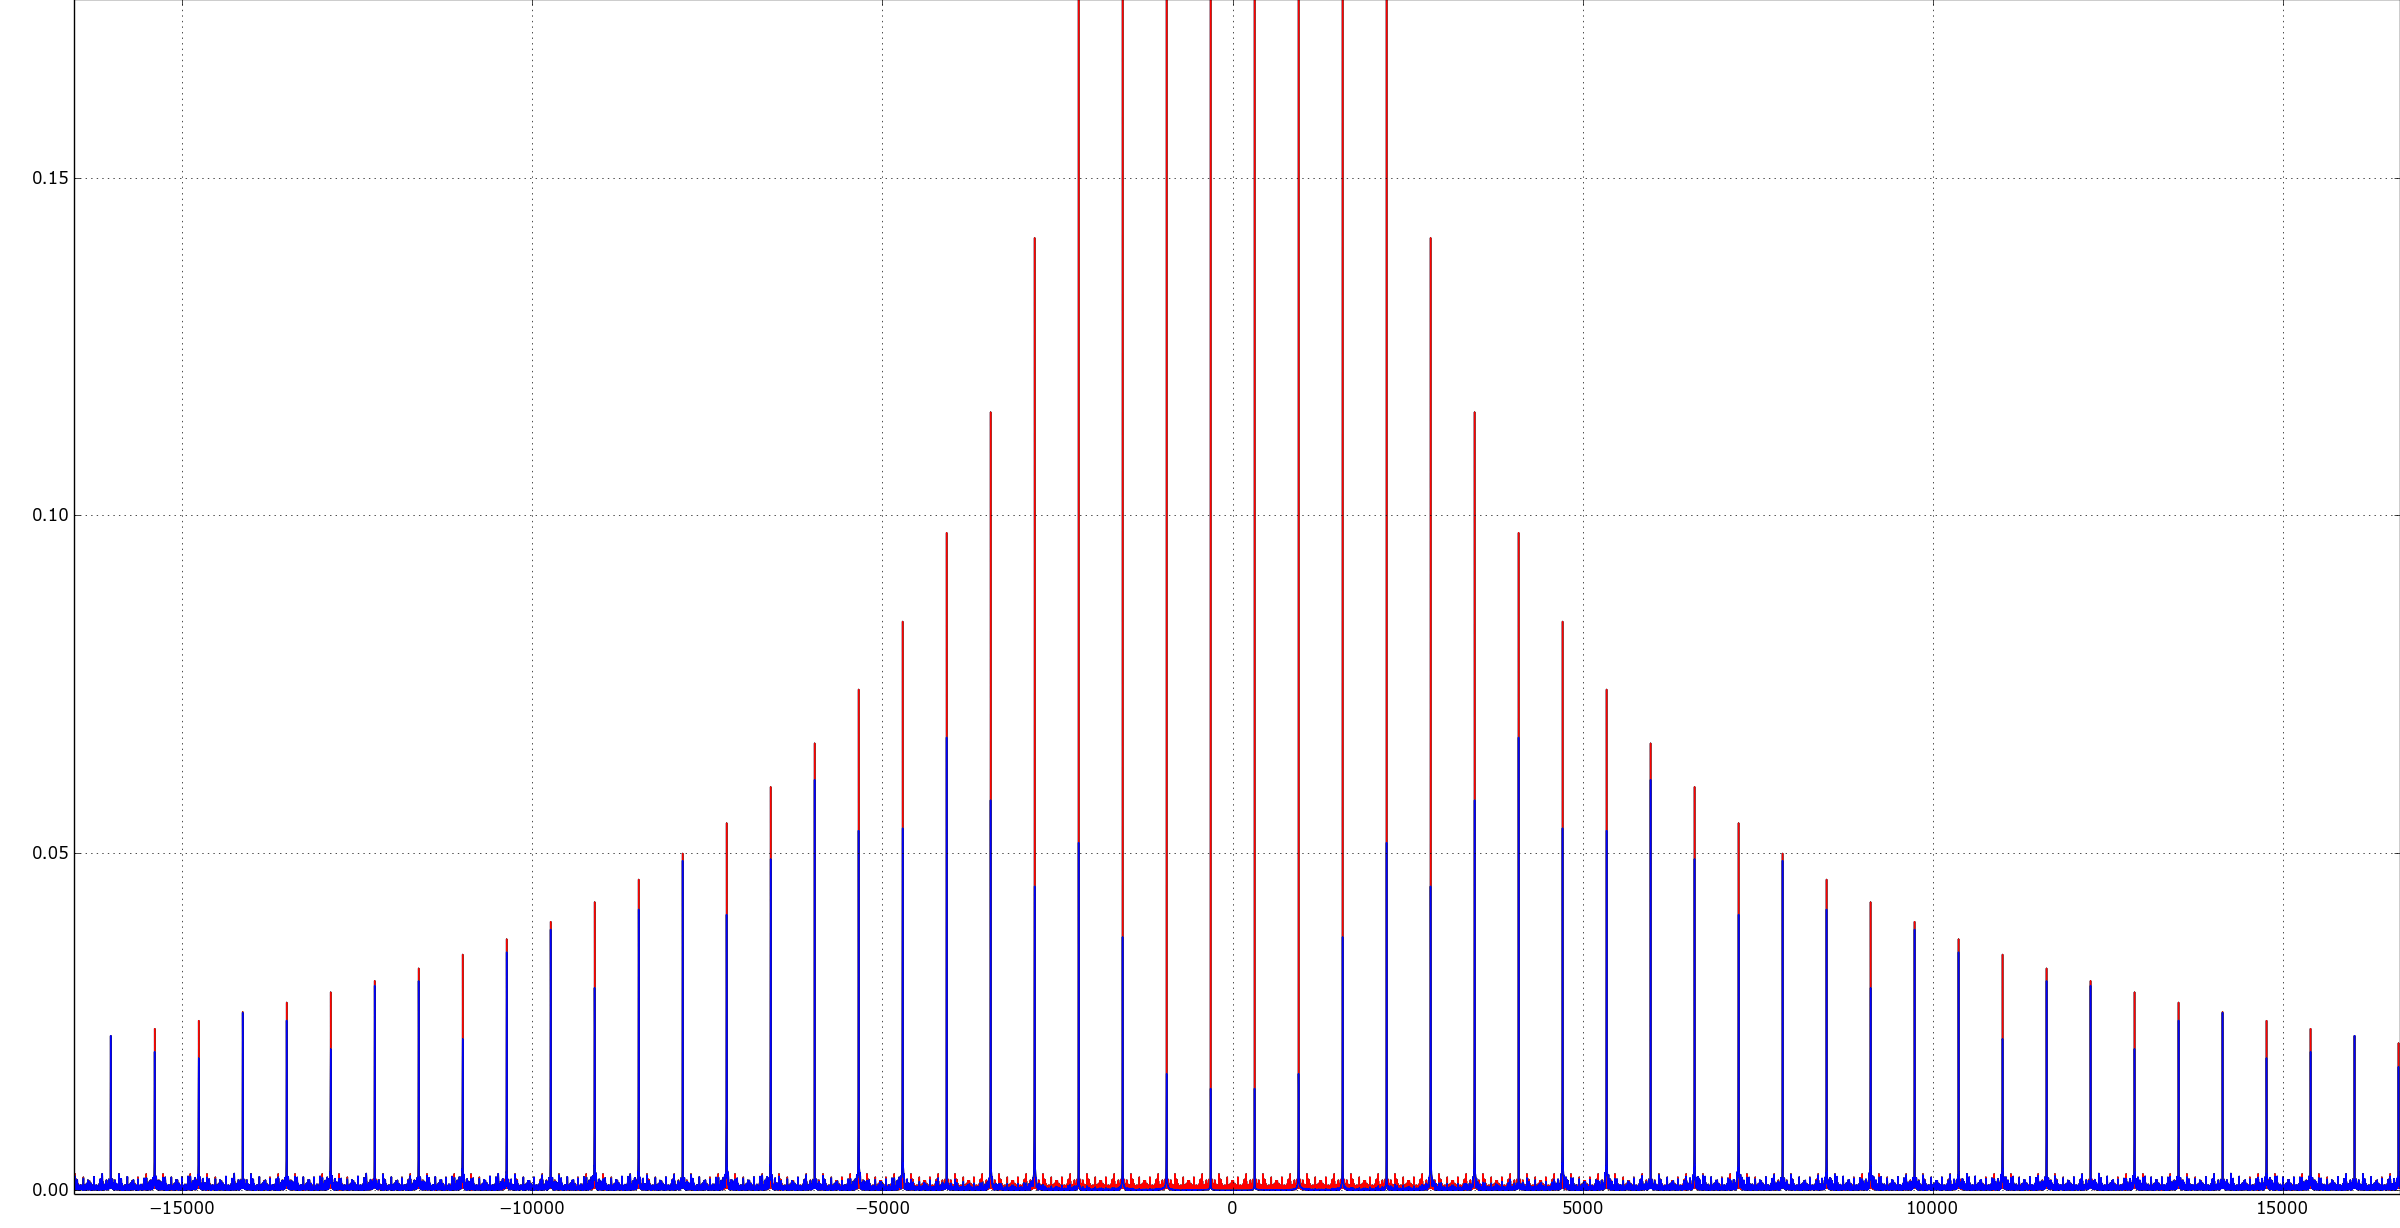
\includegraphics[width = 0.5\linewidth]{prints/filtragem_imperfeita.png}   
    \caption{Comparação entre a resposta em frequência (angular, \(\omega = 2\pi f\)) do sinal \(p\) original (\textcolor{Red}{a vermelho}) e do sinal \(p\) atenuado pelo filtro passa-baixo (\textcolor{Blue}{a azul}).}
    \label{fig:filtragem_imperfeita}
\end{figure}
%\fi

Após obtidas as conclusões teóricas sobre o sinal \(p\) transformado pelos filtros, foram ouvidos\footnotemark[6] os três respetivos sinais: \(p\), \(sistema_4(p)\) e \(sistema_5(p)\). 

Deste modo, foi confirmado mais uma vez que após a passagem do sinal \(p\) pelo filtro passa-baixo, é reproduzido um som \textit{grave} (onde predominam as zonas de variação lenta). Enquanto que, após o efeito do filtro passa-alto é audível um som \textit{agudo} (onde predominam as zonas de variação rápida) tal como esperado.

\footnotetext[6]{Estes sinais podem ser ouvidos no seguinte \href{https://drive.google.com/drive/folders/1zF89tRzYLYhmd-iCUB2yqHtHsHAs0El5?usp=sharing}{link externo}.}
%}}

\clearpage
%------------------------------------------------------%
\subsubsection{(R8) Passa-banda}
\label{subsubsec:R8}
\textbf{Verifique que a saída do filtro passa-banda tem, localmente, a forma aproximada duma sinusóide. Verifique que a amplitude dessa sinusóide varia no tempo, de forma sinusoidal também. Meça o valor aproximado das frequências dessas sinusóides. Explique por que razão a saída do filtro tem esta forma e os valores de frequência encontrados.}
\paragraph{Resposta:} %{{
Ao visualizar o sinal \textit{p}, bem como a parte imaginária e real da sua \(\mathcal{TF}\{p\}(j\omega) = \mathcal{P}(j\omega)\) foi possível concluir que este é um sinal real e ímpar\footnotemark[7], e como consequência devemos considerar na dedução, que a sua Transformada de Fourier apenas tem componente imaginária pura.

\begin{figure}[ht]
    \centering
    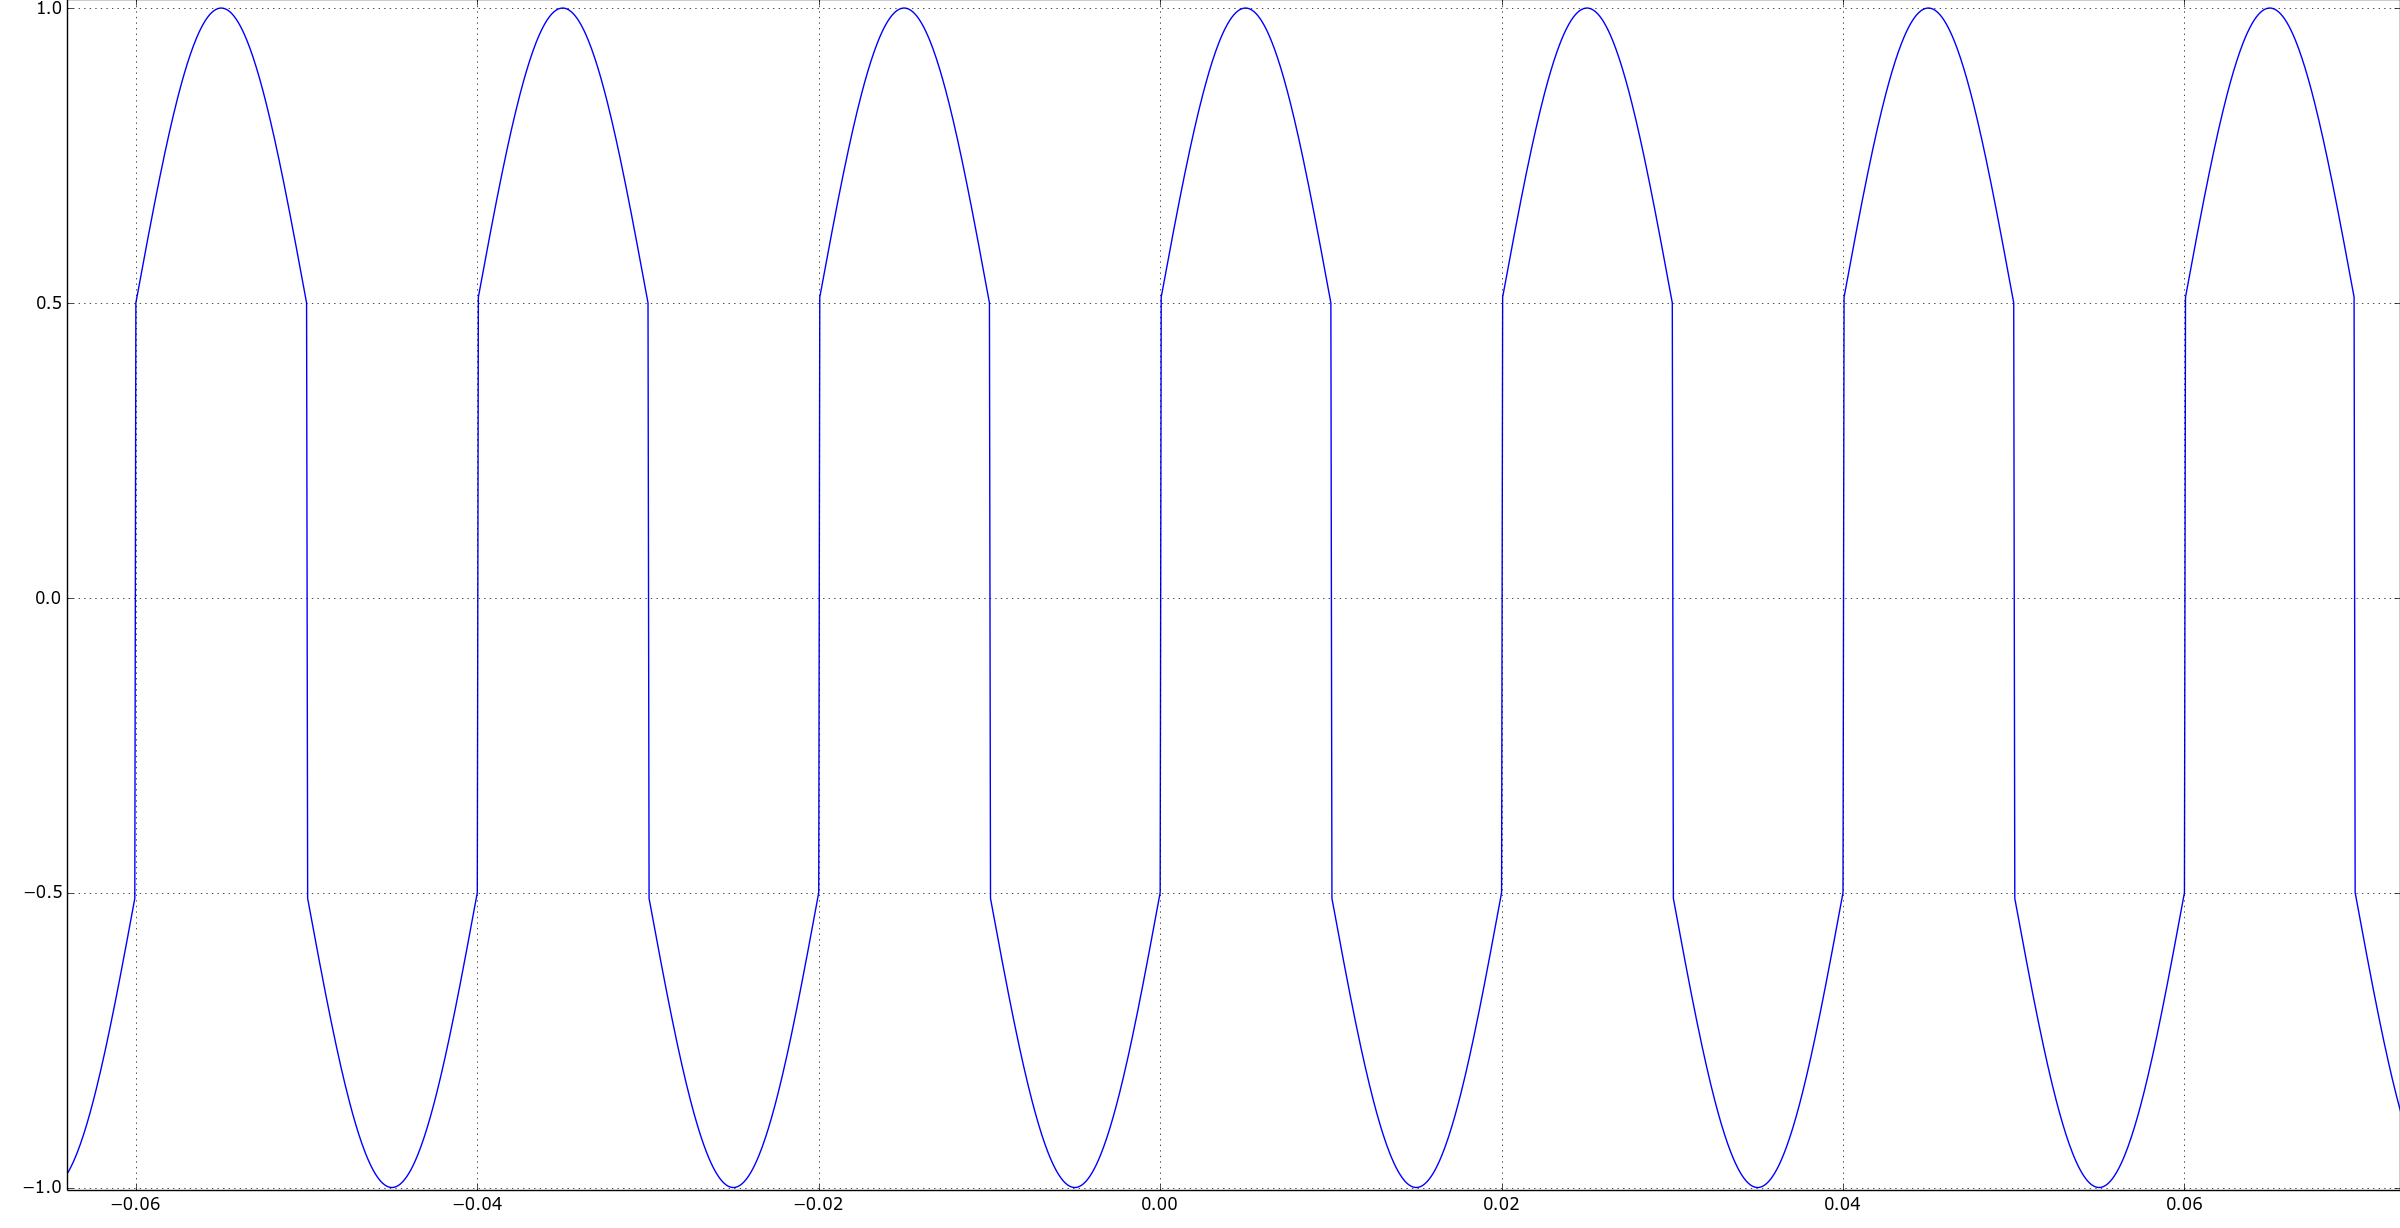
\includegraphics[width = 0.5\linewidth]{prints/sinal_p.png}   
    \caption{Sinal \textit{p} ao longo do tempo.}
    \label{fig:sinal_p}
\end{figure}

\begin{figure}[ht] 
    \begin{subfigure}[b]{0.5\linewidth}
        \centering
        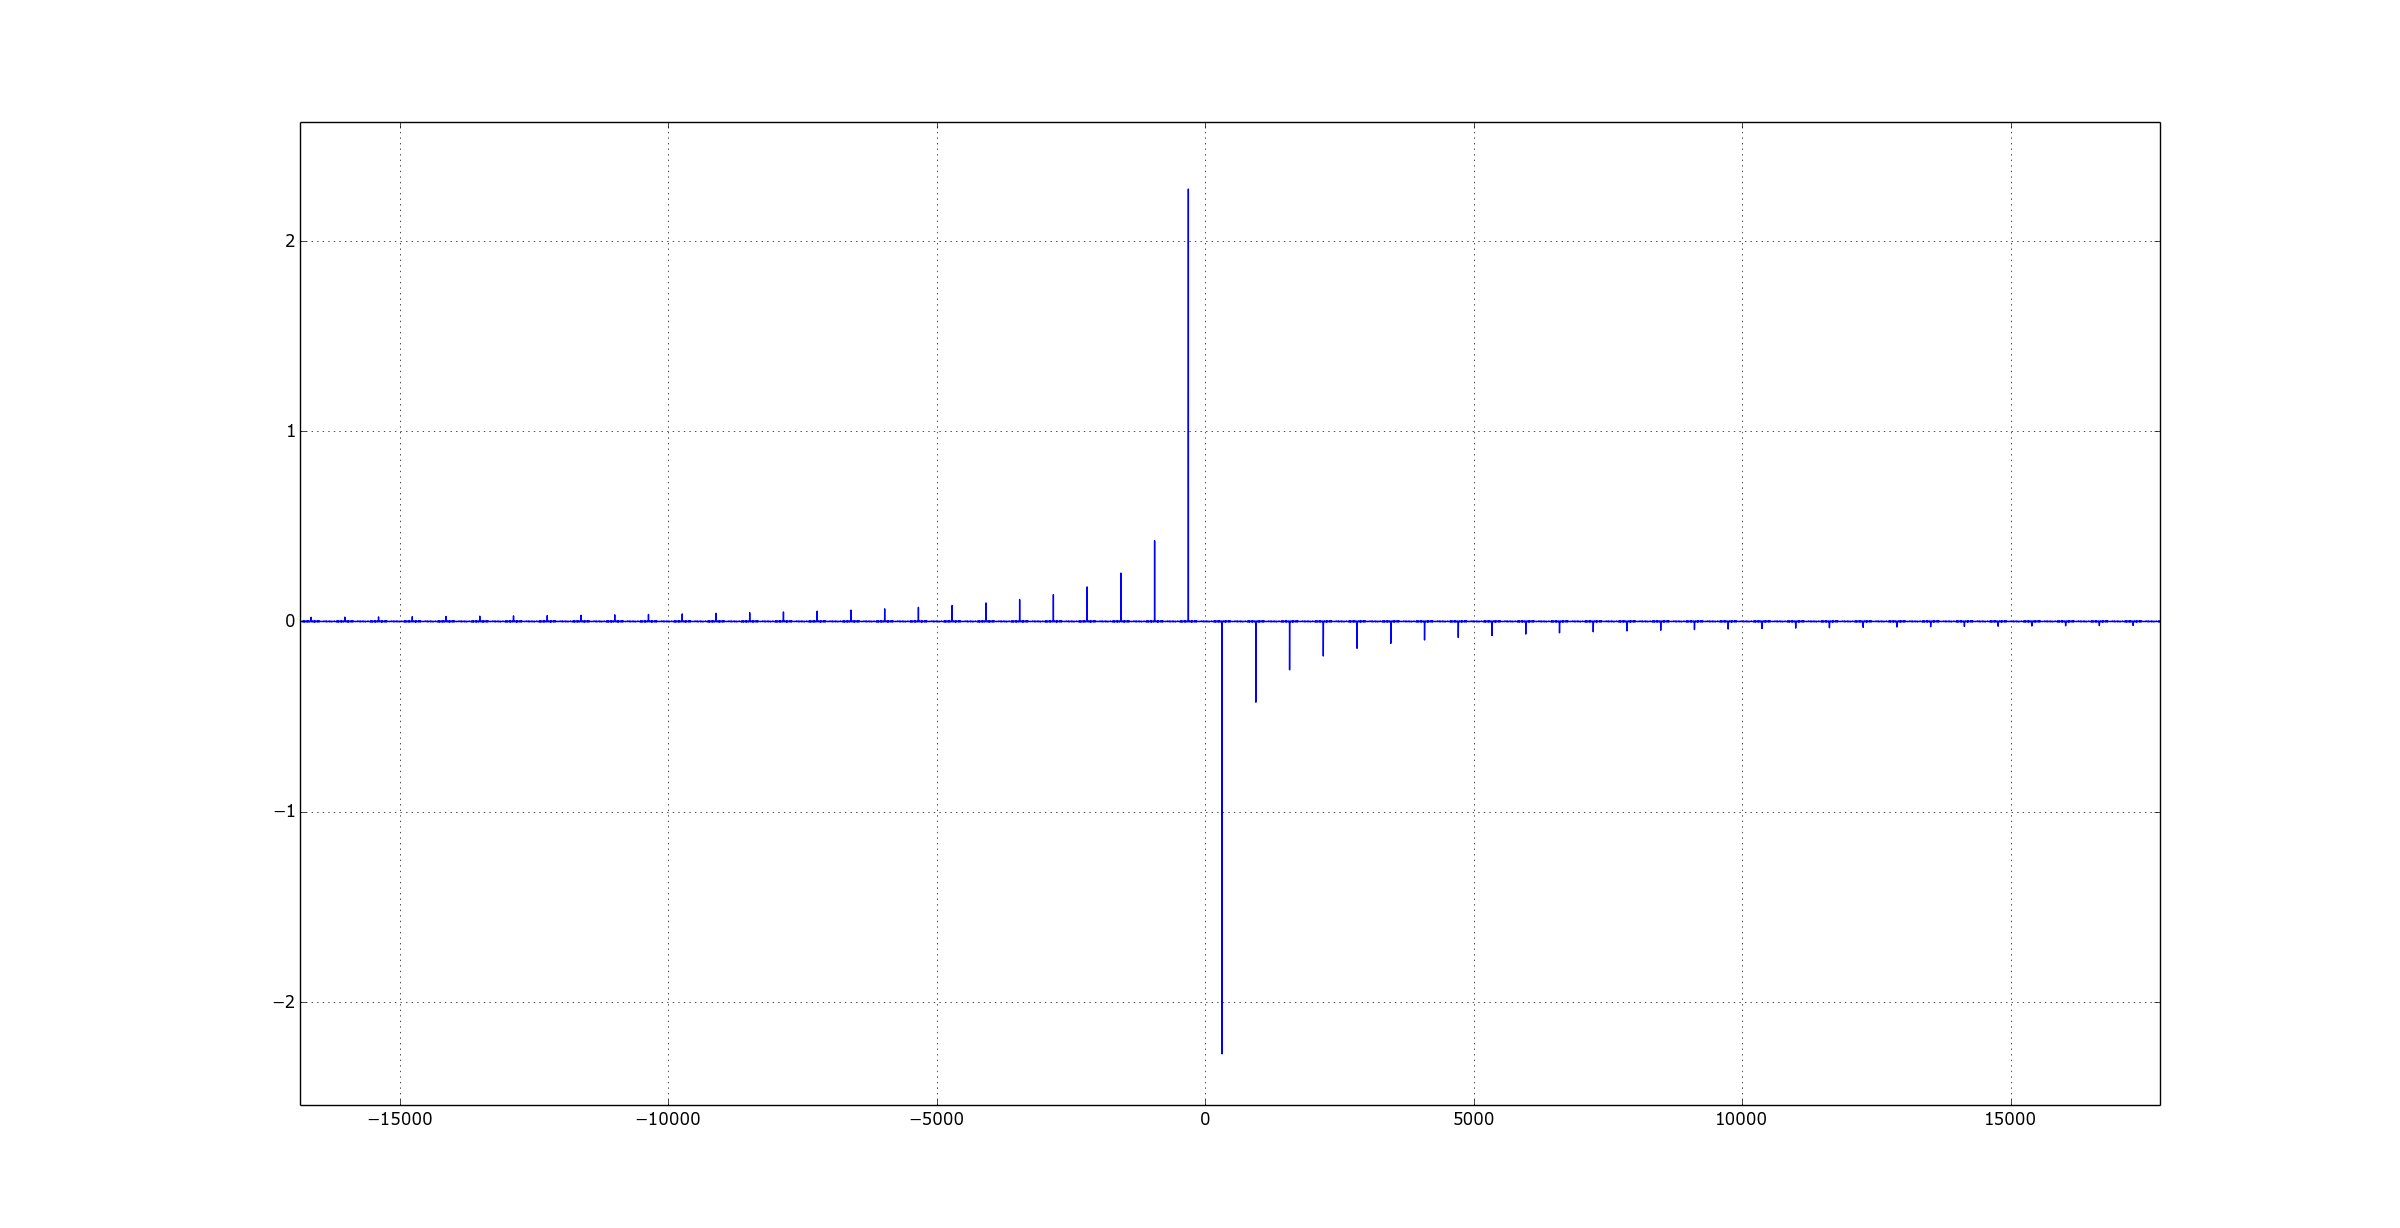
\includegraphics[width=1\linewidth]{prints/P_imag.png}
        \caption{\(\mathbb{I}m \{\mathcal{P}(j\omega)\)\}.} 
        \label{fig:P_imag} 
        %%\vspace{4ex}
    \end{subfigure}%% 
    \begin{subfigure}[b]{0.5\linewidth}
        \centering
        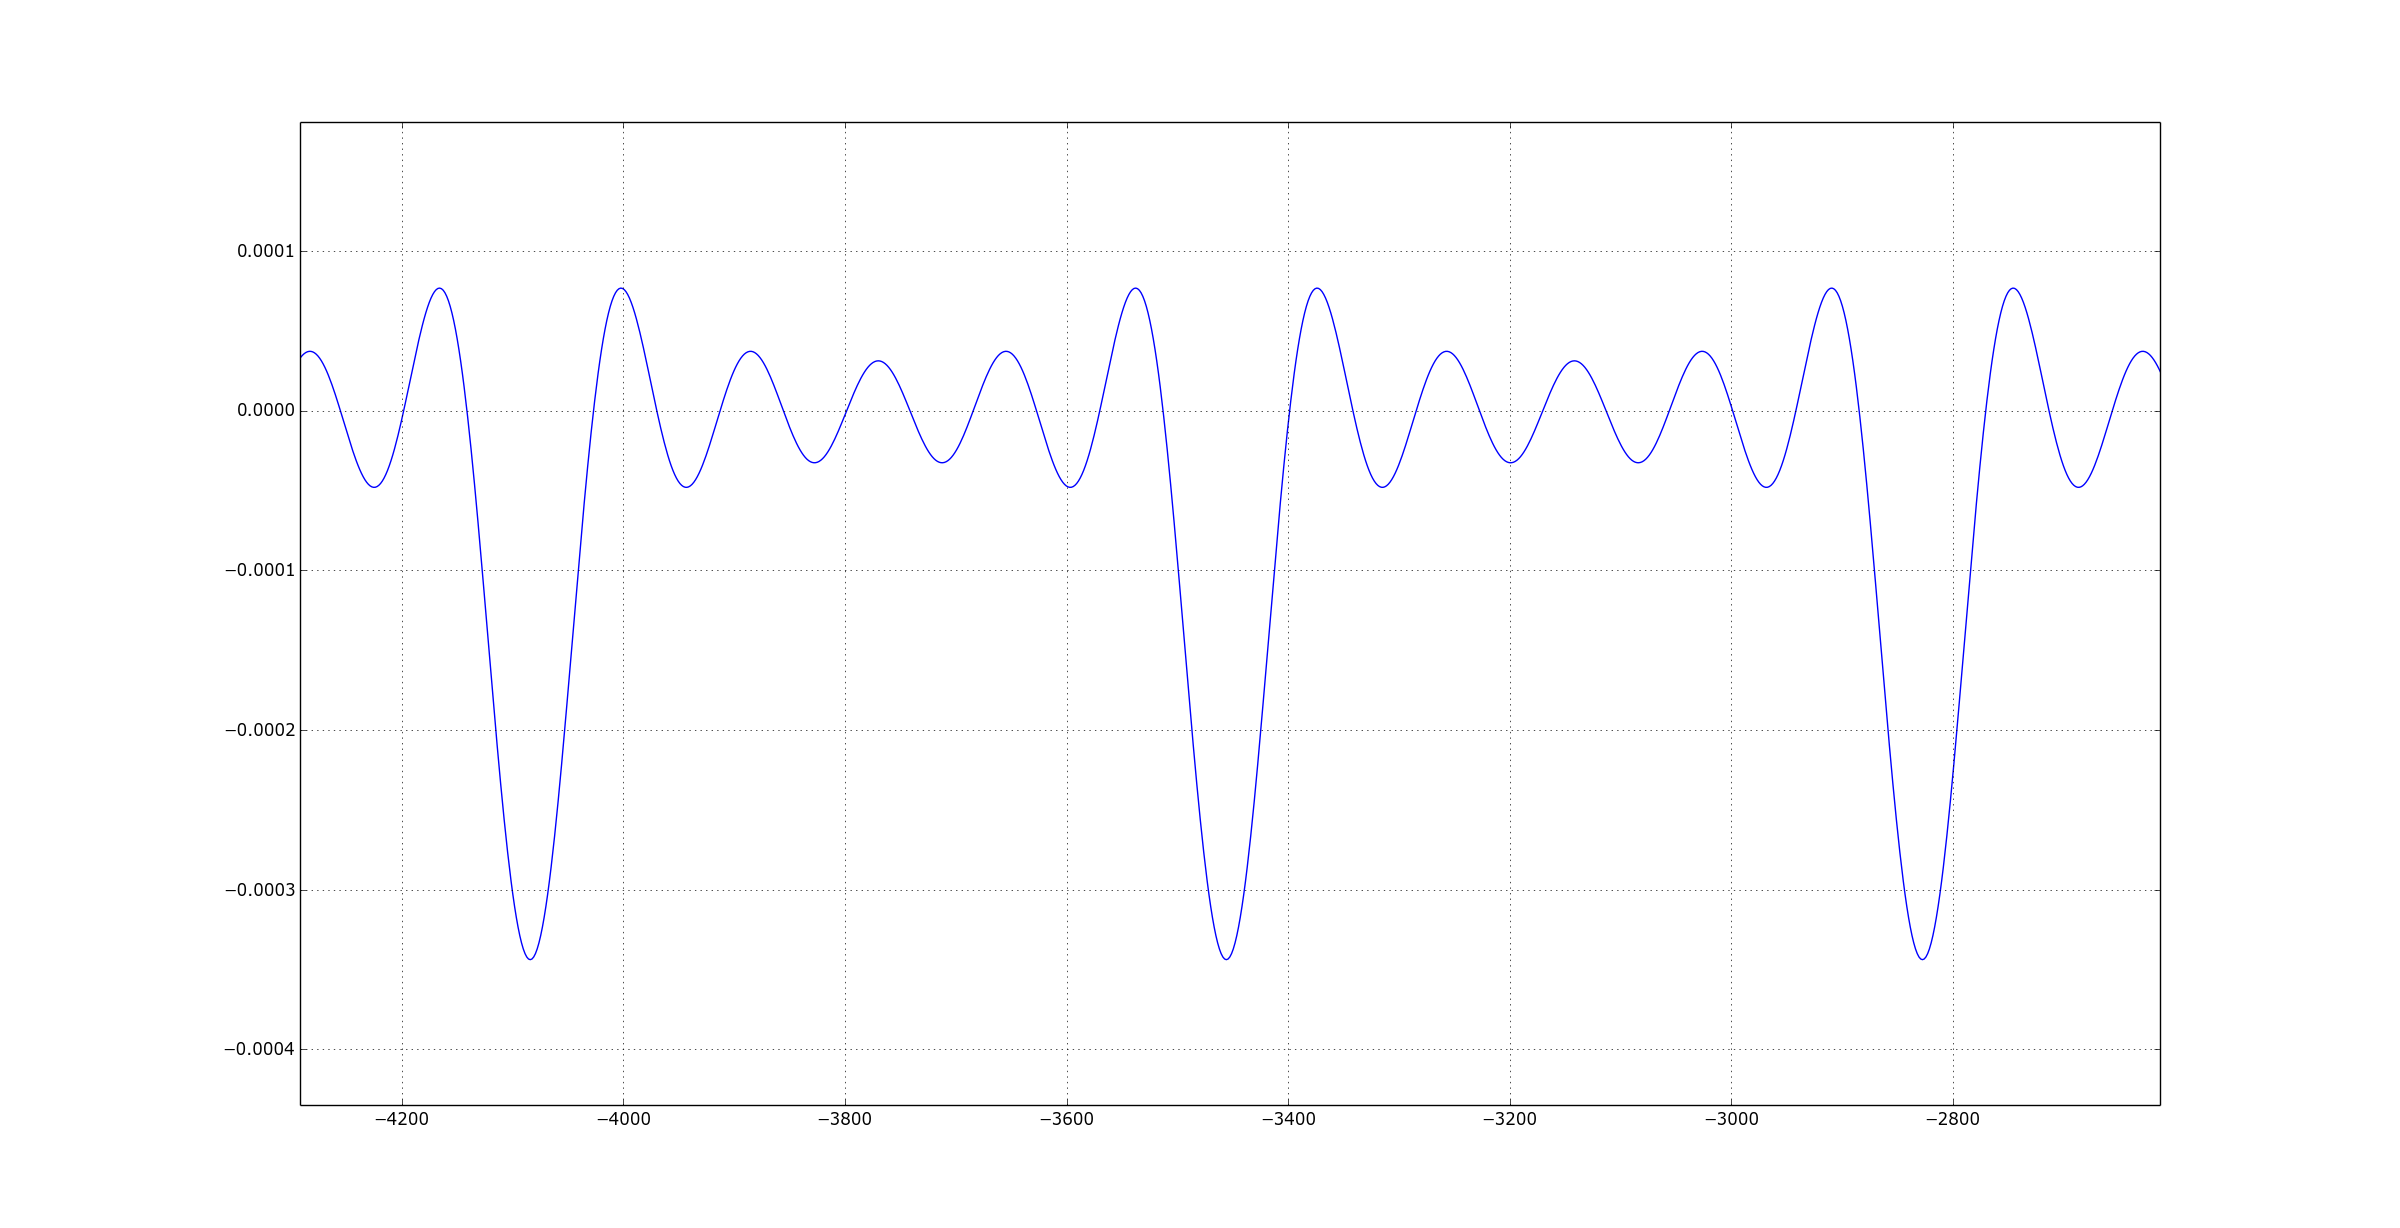
\includegraphics[width=1\linewidth]{prints/P_real.png} 
        \caption{\(\mathbb{R}e \{\mathcal{P}(j\omega)\)\}.} 
        \label{fig:P_real} 
        %%\vspace{4ex}
    \end{subfigure} 
    \caption{Representação no domínio da frequência (angular, \(\omega = 2\pi f\)) das partes imaginária e real do sinal \textit{p}.}
    \label{fig:multiplas_5}
\end{figure}

Agora, com um conhecimento mais profundo sobre o sinal \textit{p}, procedeu-se à visualização do modulo de \( \mathcal{P}(j\omega)\) e de \(\mathcal{H}(j\omega) \) no mesmo gráfico, em que \(\mathcal{H}(j\omega)\) é a função de transferência do nosso SLIT passa-banda com \(\vert f_{c1}\vert = 800\ Hz \ \text{e}\ \vert f_{c2}\vert = 1000\ Hz\). Deste modo, concluiu-se que as únicas frequências do sinal \textit{p} que sobrevivem ao filtro são as frequências \(\pm 850\ Hz\ \text{e}\ \pm 950\ Hz\) como visivel na \hyperref[fig:sistema6_absH]{Fig. 17}.

\footnotetext[7]{\(\mathbb{R}e \{\mathcal{P}(j\omega)\} \approx 0\) (um sinal real e ímpar teria, teoricamente, a parte real da sua Transformada de Fourier nula). Foi concluído que esta irregularidade no sinal \textit{p} advém do sistema laboratorial em \textit{Python} (que apenas consegue aproximar os sinais) ou que se trata de uma impureza presente.}

\clearpage

Isto porque, a saída \(y(t)\) do nosso \(sistema_6\), em frequência, pode ser vista como:

\[\mathcal{TF}\{y(t)\}(j\omega) = \mathcal{Y}(j\omega) = \mathcal{TF}\{p(t) * h(t)\}(j\omega) = \mathcal{P}(j\omega) \cdot \mathcal{H}(j\omega) \]

Deste modo, observando a parte real e imaginária do sinal resultante em frequência, i.e., \(\mathcal{P}(j\omega) \cdot \mathcal{H}(j\omega)\), concluí-se que estamos num caso bastante peculiar, como apresentado nas seguintes \hyperref[fig:sistema6_absH]{Fig. 17} e \hyperref[fig:multiplas_6]{Fig. 18}.

\begin{figure}[ht]
    \centering
    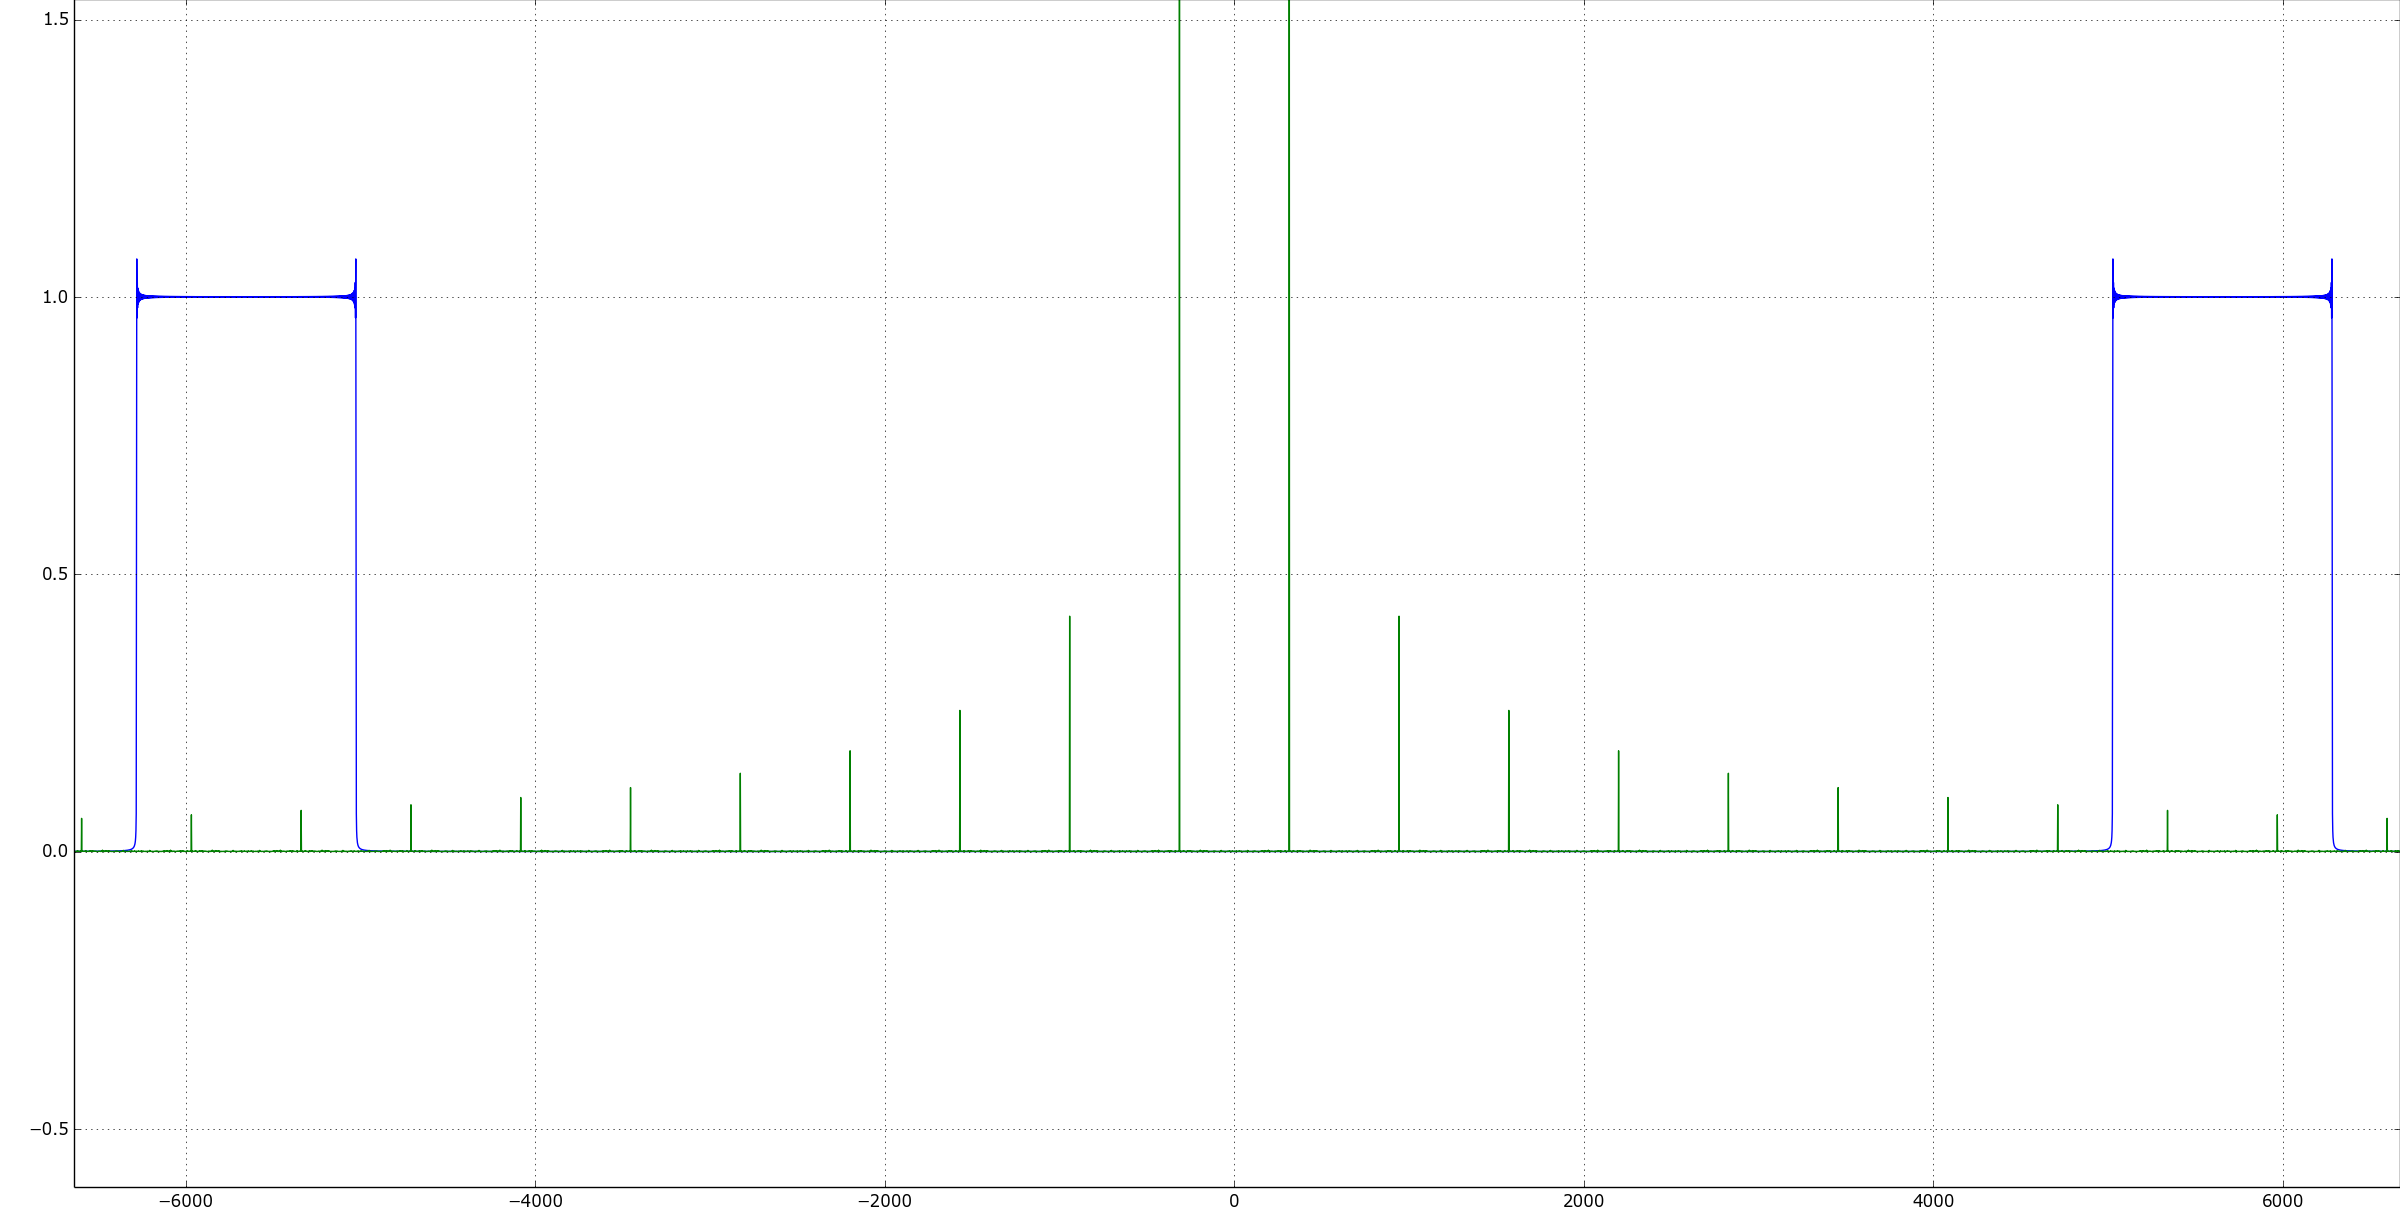
\includegraphics[width = 0.5\linewidth]{prints/sistema6_absH.png}   
    \caption{Gráficos de \(\vert \mathcal{P}(j\omega)\vert\) e \(\vert \mathcal{H}(j\omega)\vert\) sobrepostos (em frequência angular).}
    \label{fig:sistema6_absH}
\end{figure}

\begin{figure}[ht] 
    \begin{subfigure}[b]{0.5\linewidth}
        \centering
        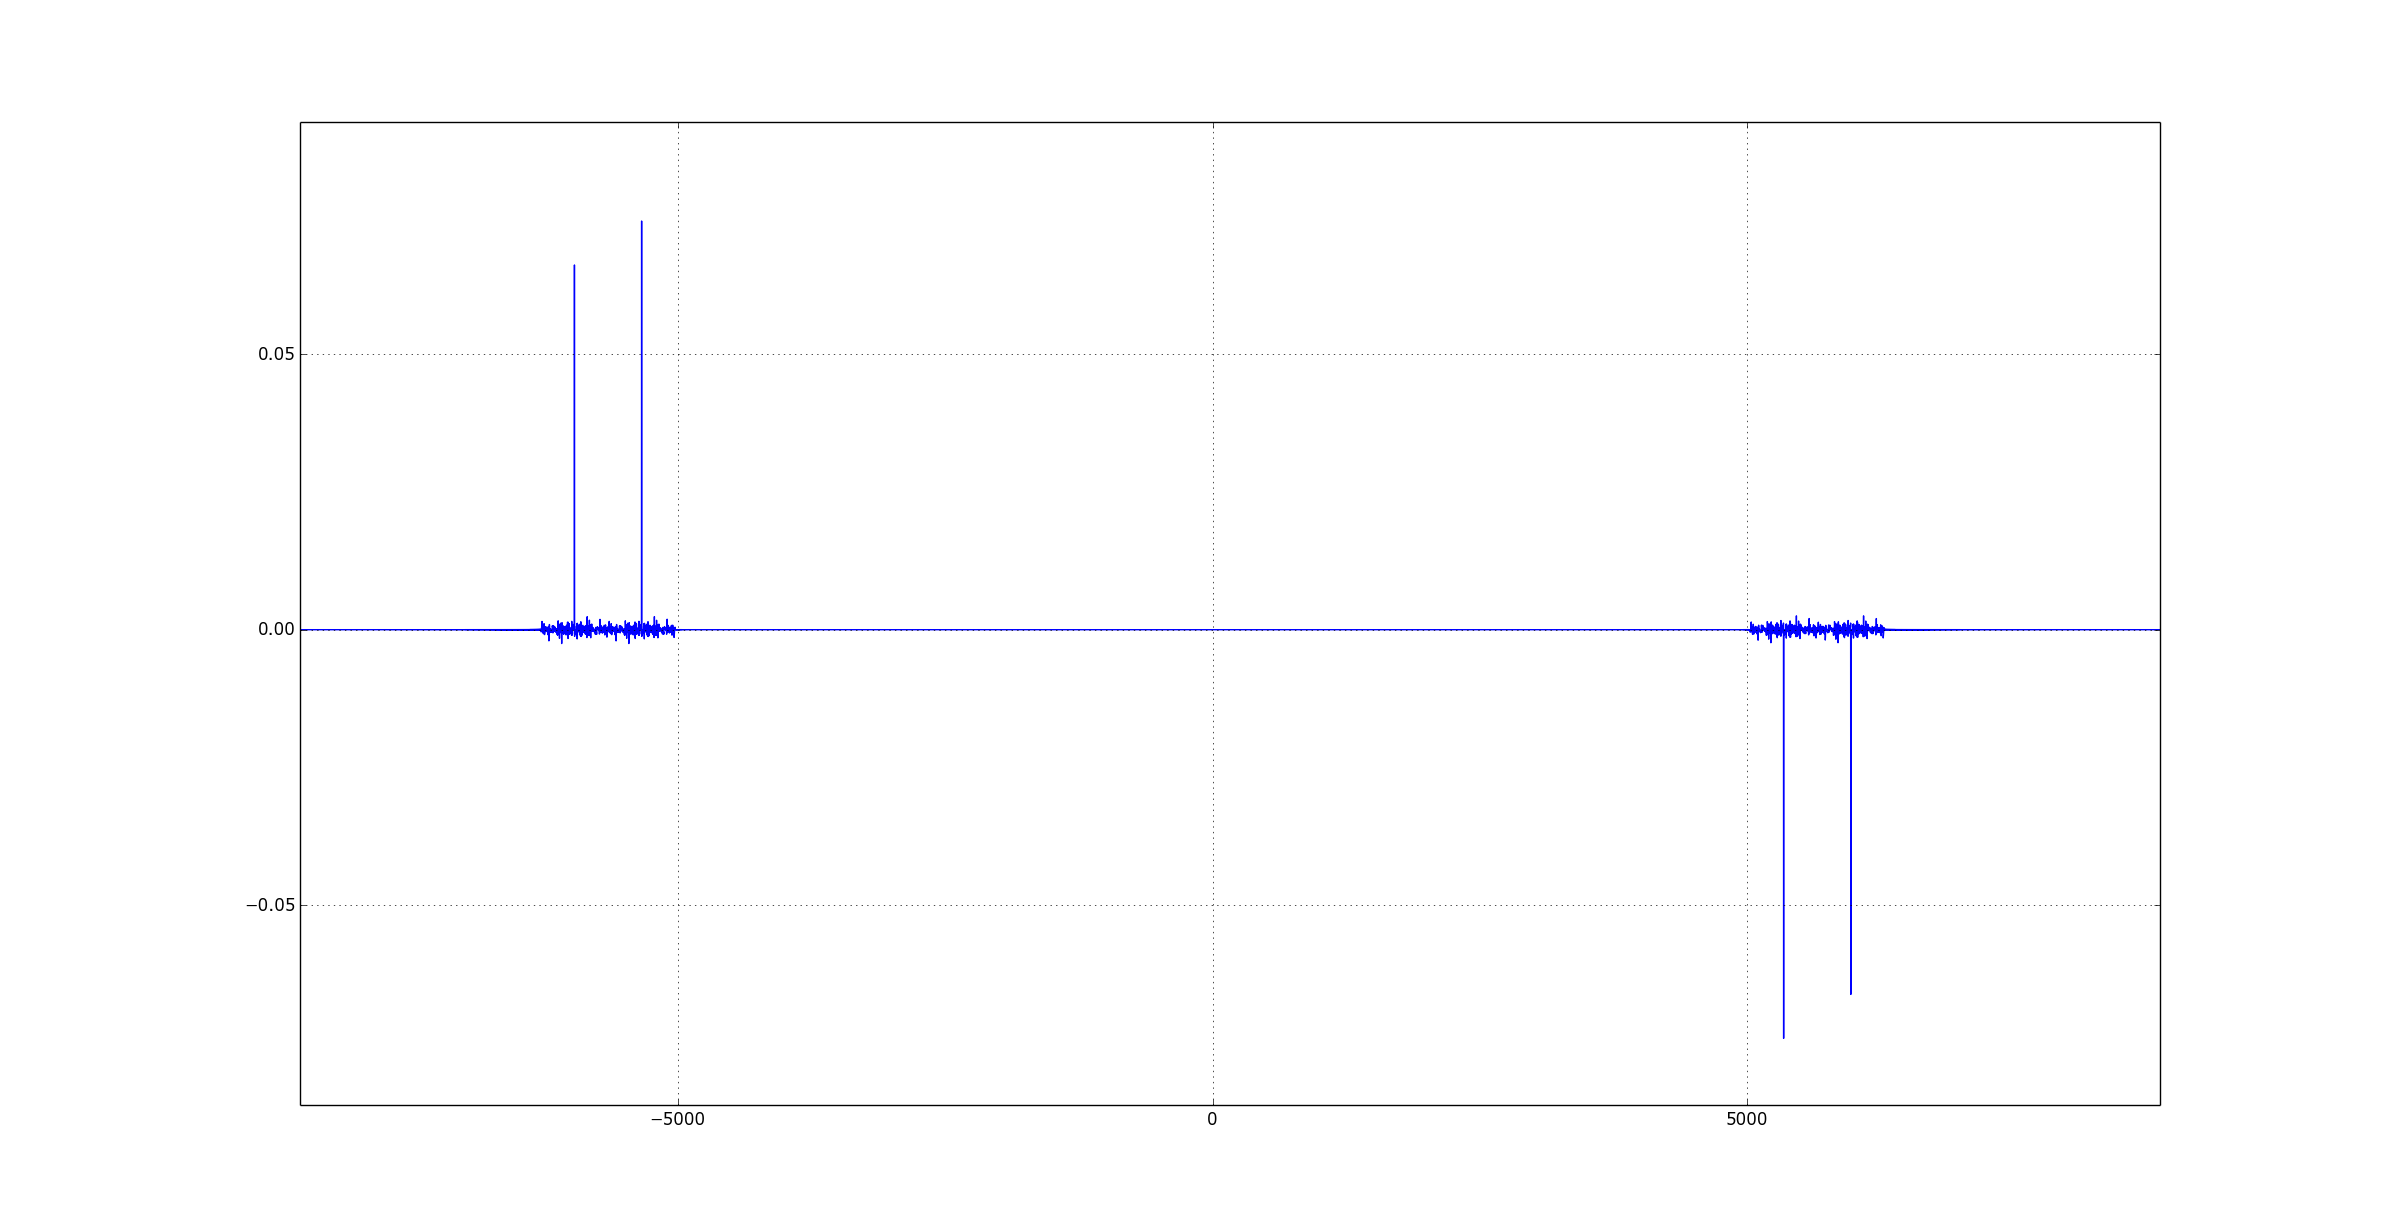
\includegraphics[width=1\linewidth]{prints/imag_H_e_P.png}
        \caption{\(\mathbb{I}m \{\mathcal{Y}(j\omega)\)\}.} 
        \label{fig:imag_H_e_P} 
        %%\vspace{4ex}
    \end{subfigure}%% 
    \begin{subfigure}[b]{0.5\linewidth}
        \centering
        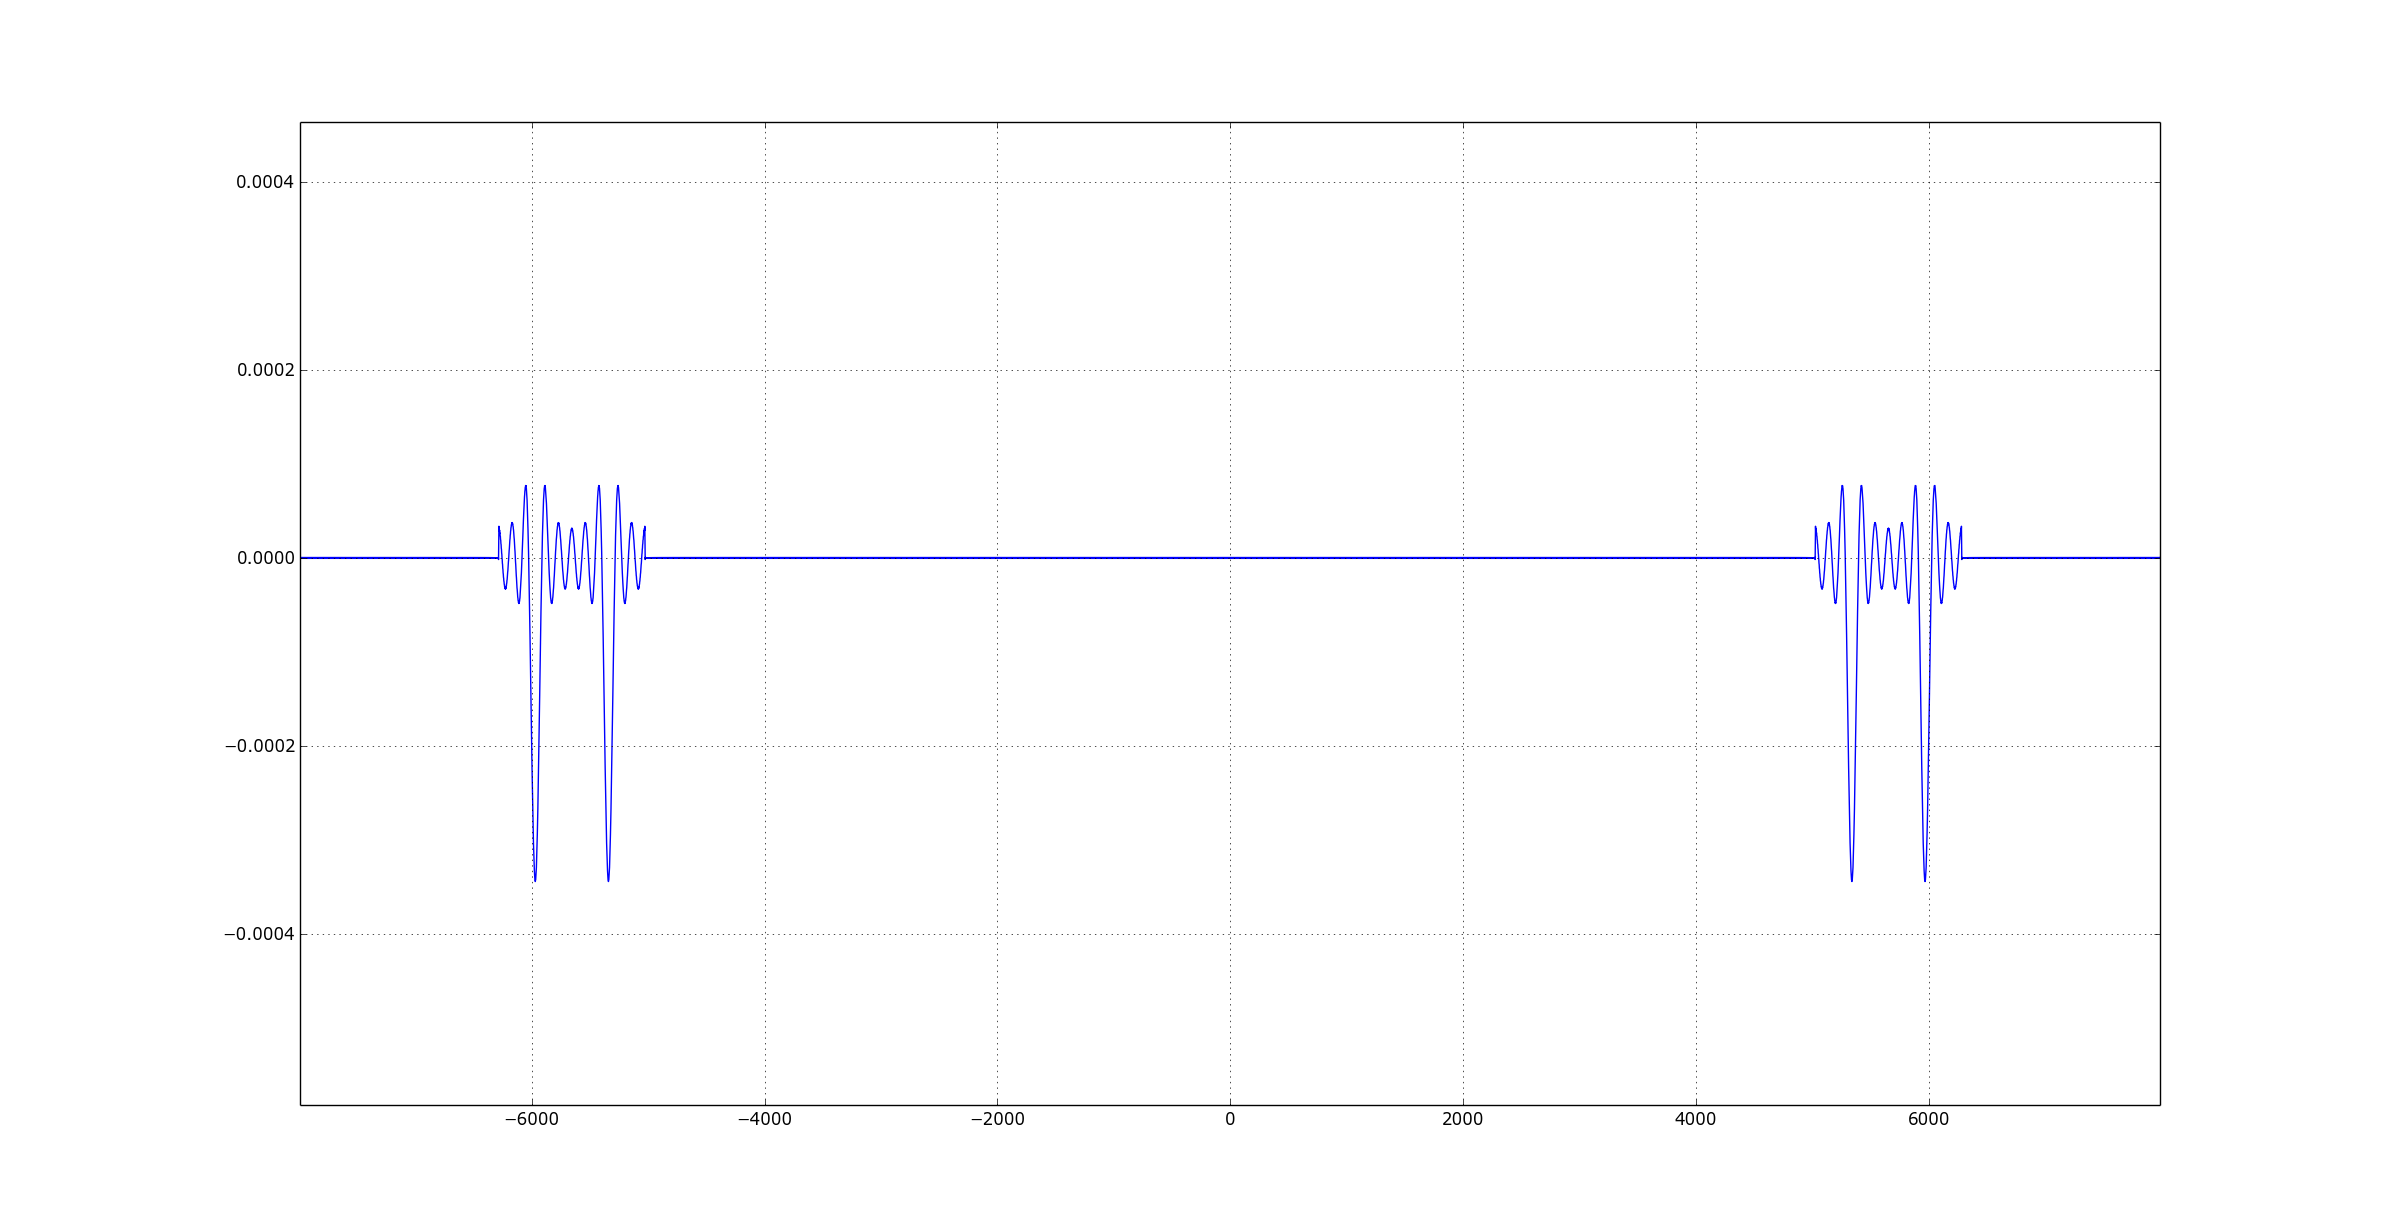
\includegraphics[width=1\linewidth]{prints/real_H_e_P.png} 
        \caption{\(\mathbb{R}e \{\mathcal{Y}(j\omega)\)\}.} 
        \label{fig:real_H_e_P} 
        %%\vspace{4ex}
    \end{subfigure} 
    \caption{Representação no domínio da frequência (angular, \(\omega = 2\pi f\)) das partes imaginária e real do sinal \textit{y(t)}.}
    \label{fig:multiplas_6}
\end{figure}

Atendendo às limitações do \textit{setup} em \textit{Python}, a conclusão que se deriva da \hyperref[fig:multiplas_6]{Fig. 18} é que \(\mathcal{Y}(j\omega)\) são quatro impulsos unitários deslocados, para as frequências \(-950\ Hz,\ -850\ Hz,\  850\ Hz\ \text{e}\ 950\ Hz\) como seria de esperar pela observação direta do modulo da Transformada de Fourier de \textit{p} e de \textit{h(t)} na \hyperref[fig:sistema6_absH]{Fig. 17}.

Então, é simples deduzir que estamos perante a convolução de 2 pares de impulsos unitários,
\[\mathcal{Y}(j\omega) = [a_1 \cdot \delta (\omega + \omega_1) + a_2 \cdot \delta (\omega - \omega_1)] * [ a_3 \cdot \delta (\omega + \omega_2) + a_4 \cdot \delta (\omega - \omega_2)]\]

Para que seja obtido o observado na \hyperref[fig:sistema6_absH]{Fig. 18 (a)} são impostas restrições aos coeficientes \(a_i\) com \(i = 1,2,3,4\). Por observação chegamos à conclusão que:
\[a_1 \approx a_2\ \text{, com}\ a_1\text{,}\ a_2 \in \mathbb{R}^{+}\ \text{e}\ a^{*}_3 = a_{4}\ \text{, em que}\ a_3 \in \mathbb{C}^{+}\ \text{e}\ \mathbb{R}e\{a_3\} = 0 \]

Dado que uma convolução no domínio do tempo corresponde a um produto no domínio da frequência, temos que, pela dualidade da operação, uma convolução no domínio da frequência corresponde a um produto no domínio do tempo:

\[\implies \mathcal{TF}^{-1}\{\mathcal{Y}(j\omega)\}(t) = y(t) \approx k \cdot \cos (\omega_1 \cdot t) \cdot \sin (\omega_2 \cdot t)\ \text{,}\ k \in \mathbb{R}^{+}\]
tal que, \(\omega_1 = 100 \pi \implies f_1 = 50\ Hz\ \text{e}\ \omega_2 = 1800 \pi \implies f_2 = 900\ Hz\), visto que no gráfico de \(\mathbb{I}m\{\mathcal{Y}(j\omega)\}\) os impulsos unitários são visiveis em \(\pm 850\ Hz\ \text{e}\ \pm 950\ Hz\).

\begin{figure}[H] 
    \begin{subfigure}[b]{0.5\linewidth}
        \centering
        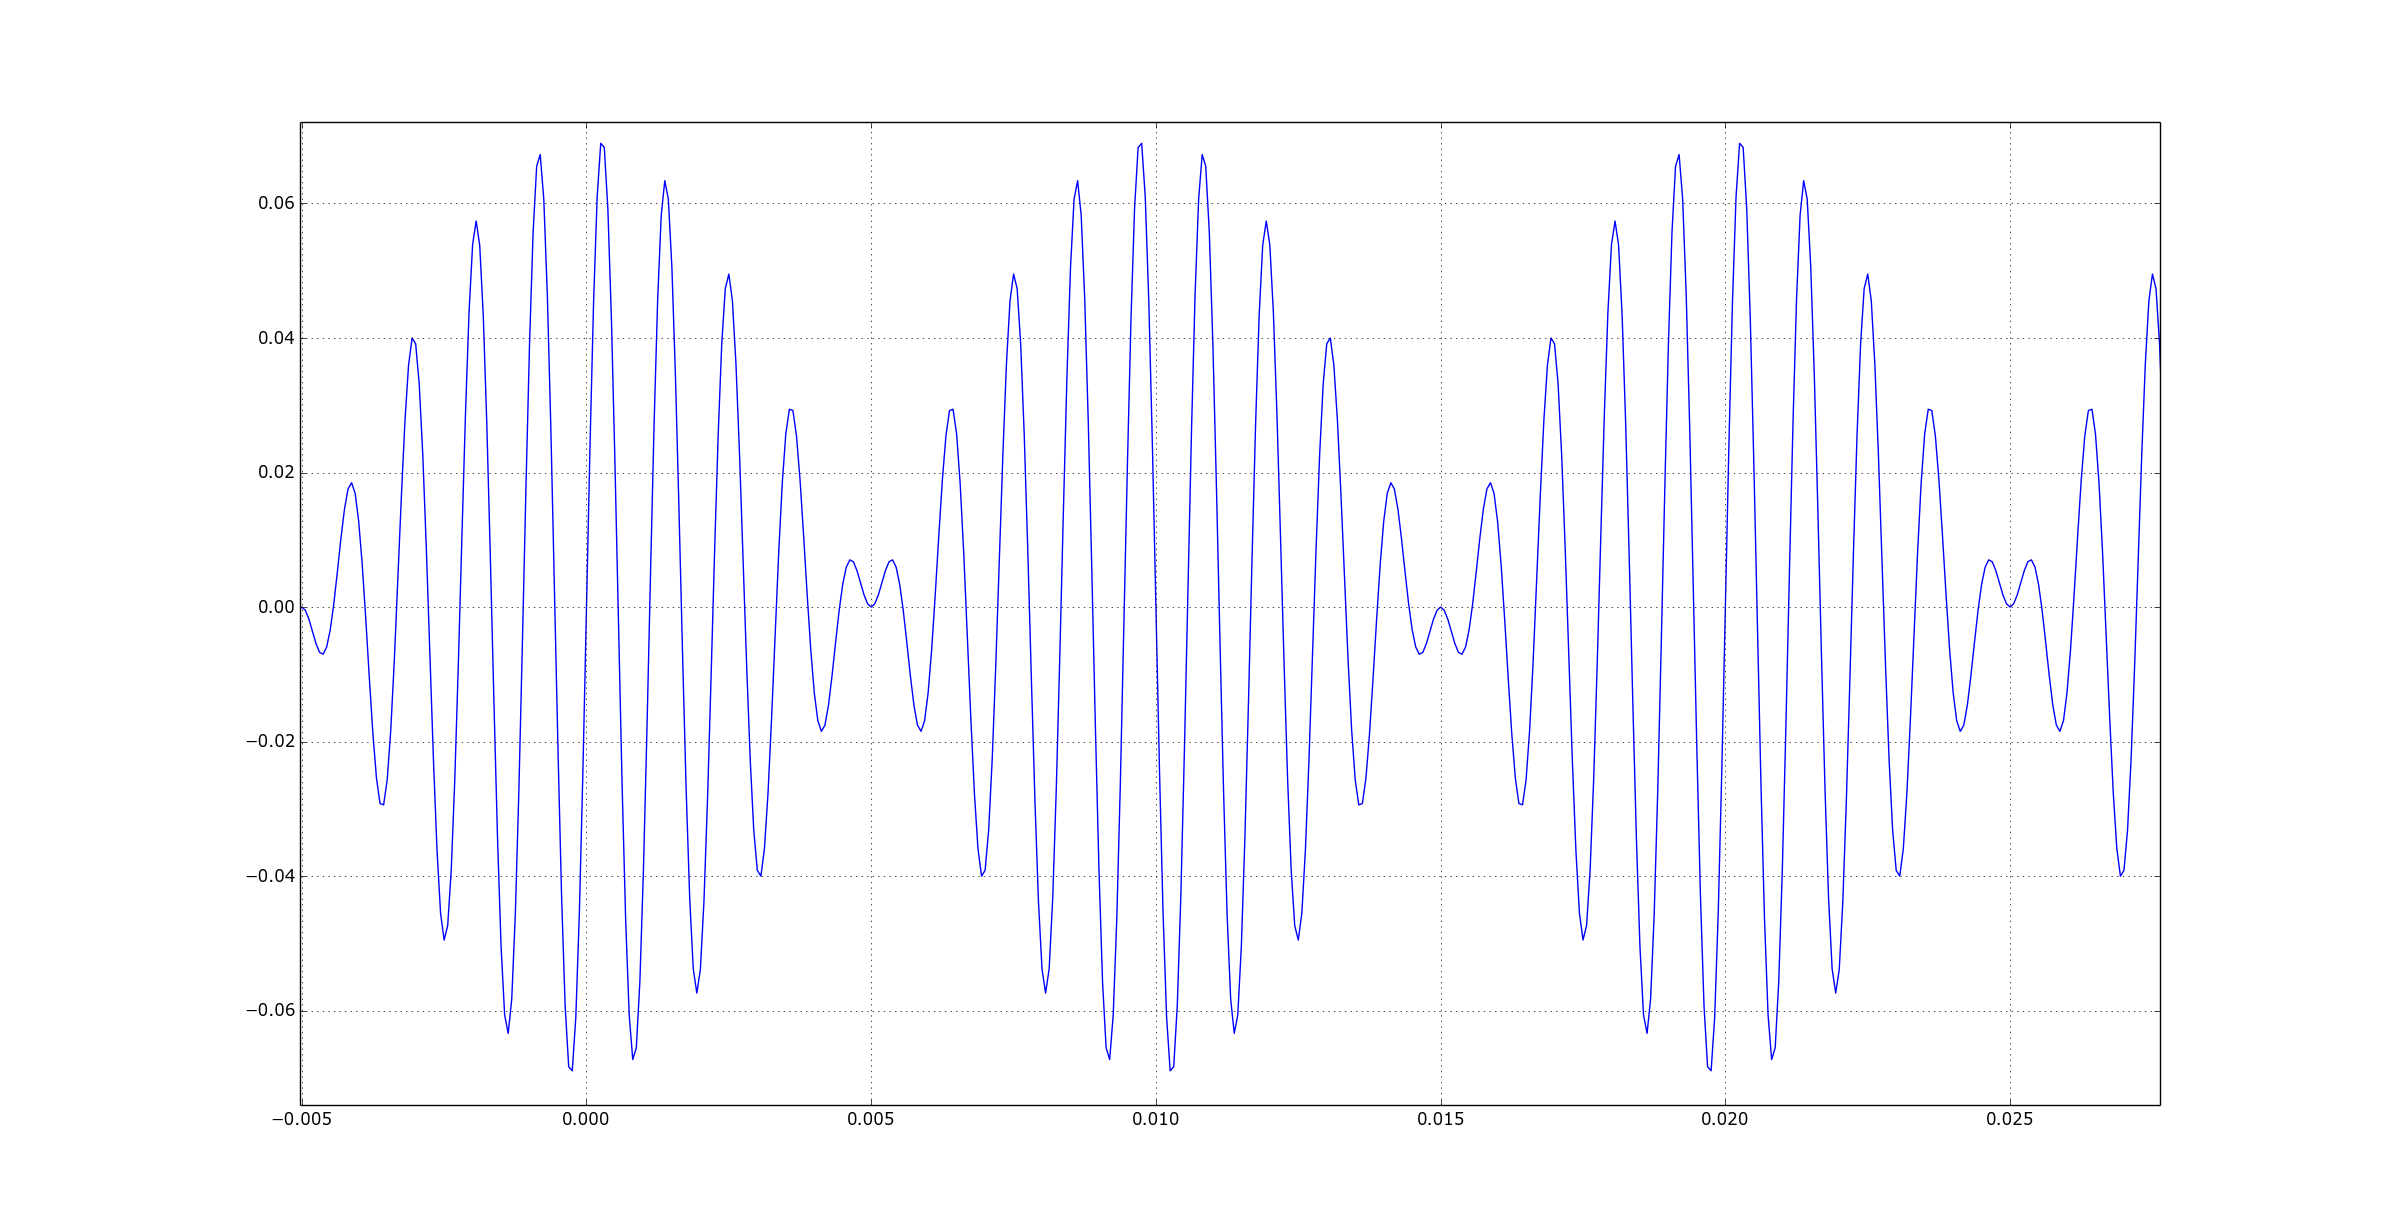
\includegraphics[width=1\linewidth]{prints/saida_experimental_sistema6.png}
        \caption{Saída aproximada, com \(k = 0.07\).} 
        \label{fig:saida_experimental_sistema6} 
        %%\vspace{4ex}
    \end{subfigure}%% 
    \begin{subfigure}[b]{0.5\linewidth}
        \centering
        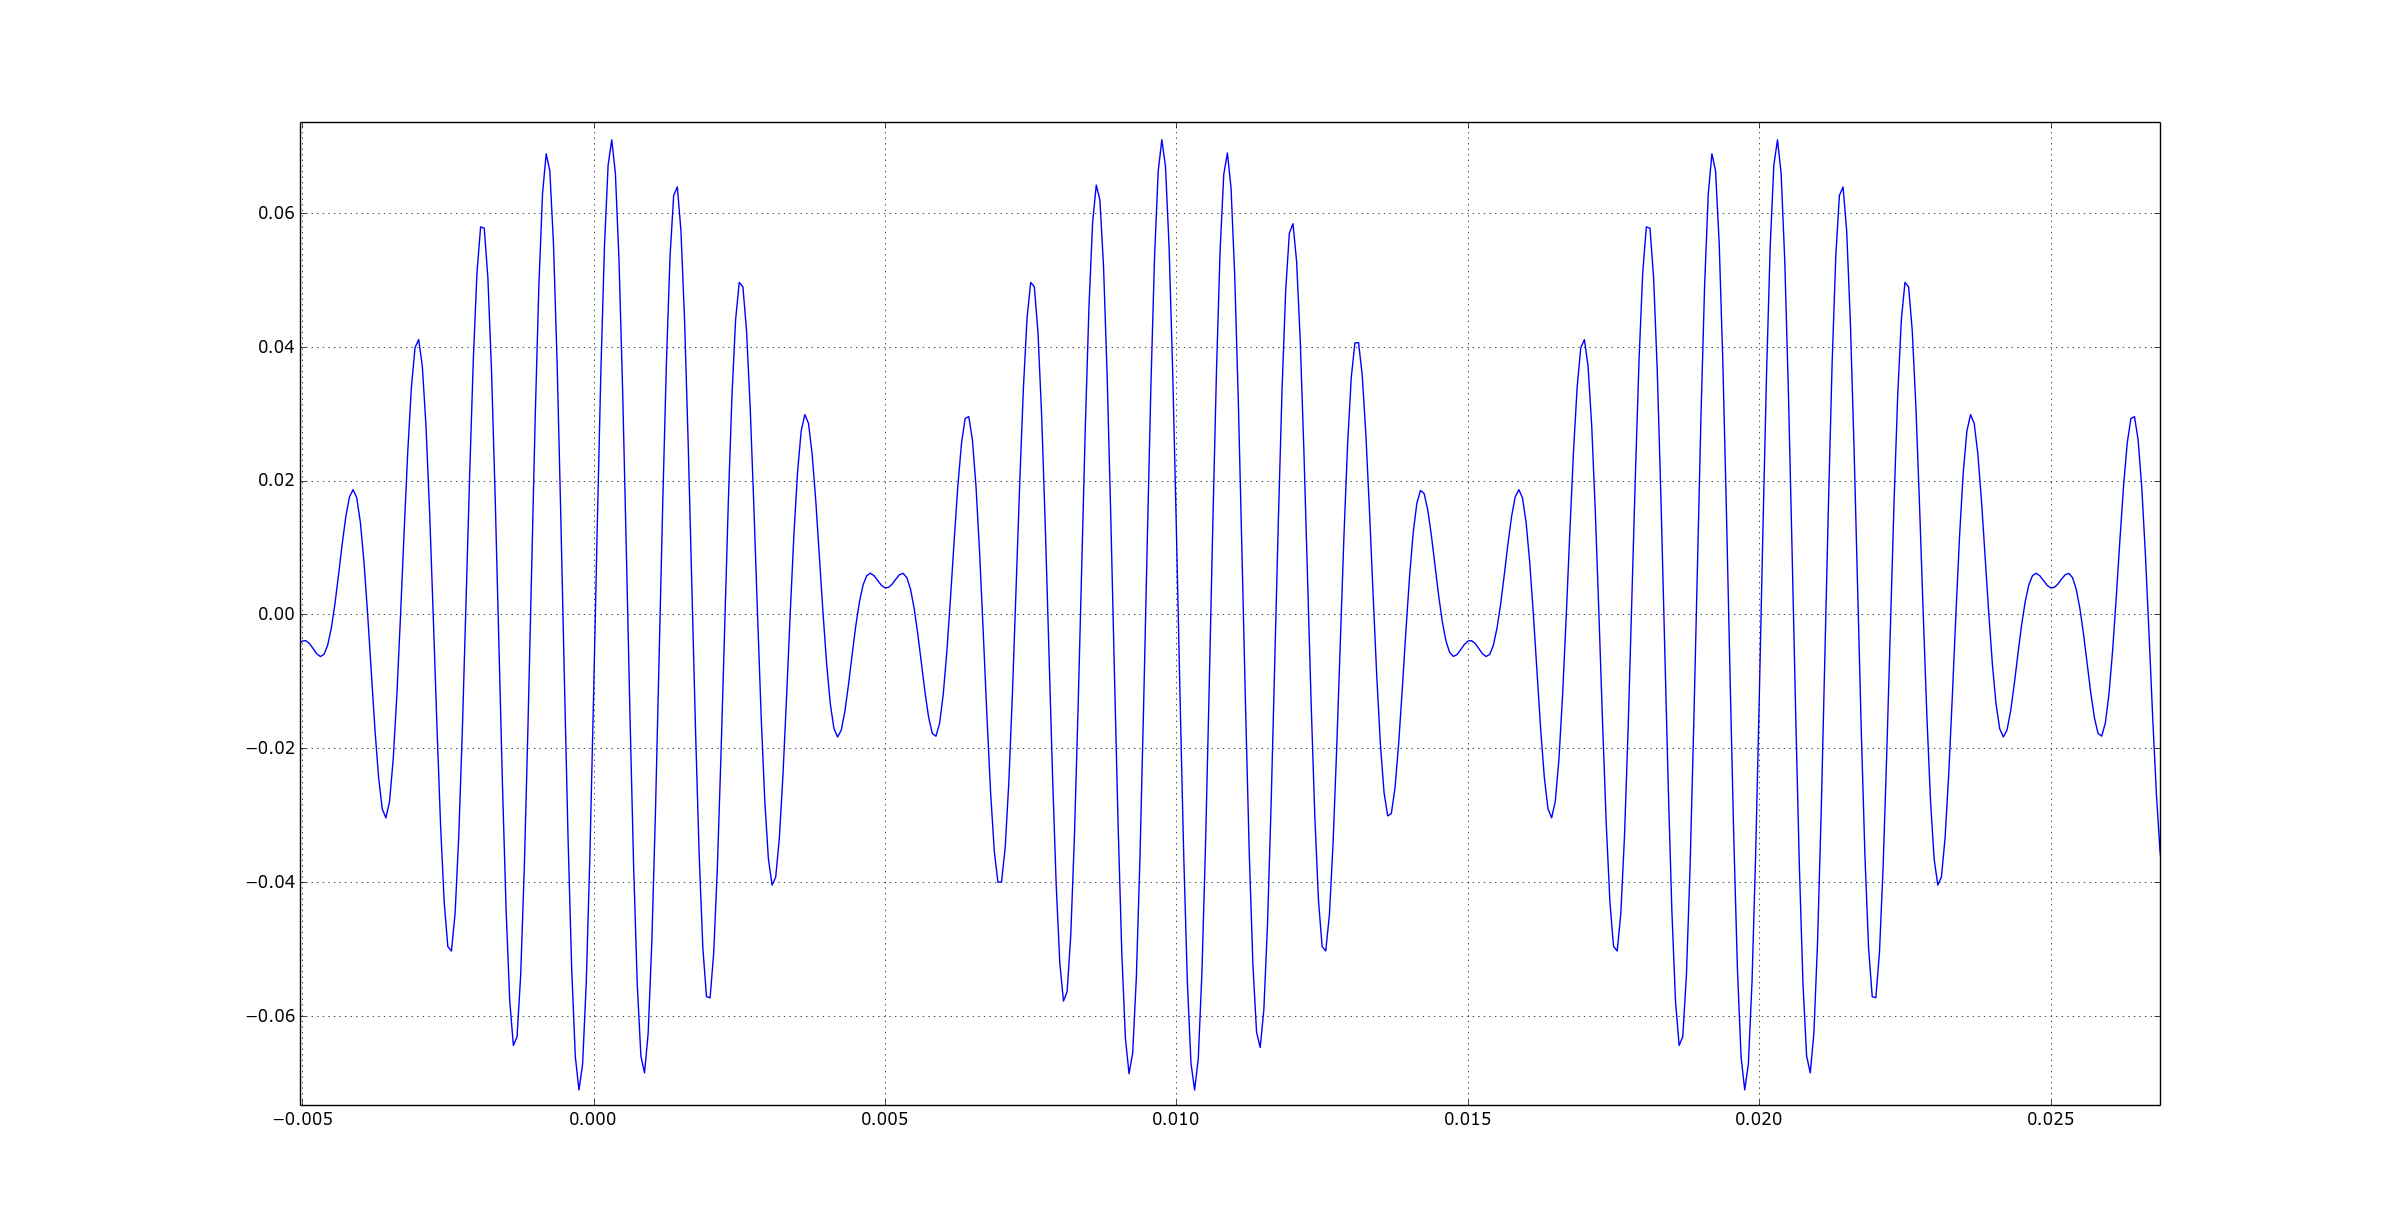
\includegraphics[width=1\linewidth]{prints/sistema6_p.png} 
        \caption{Saída produzida pelo \(sistema_6\).} 
        \label{fig:sistema6_p} 
        %%\vspace{4ex}
    \end{subfigure} 
    \caption{Comparação entre a saída aproximada com a saída produzida pelo \(sistema_6\) (relativamente ao sinal de entrada \(p\)), no domínio do tempo.}
    \label{fig:multiplas_7}
\end{figure}

\begin{figure}[ht]
    \centering
    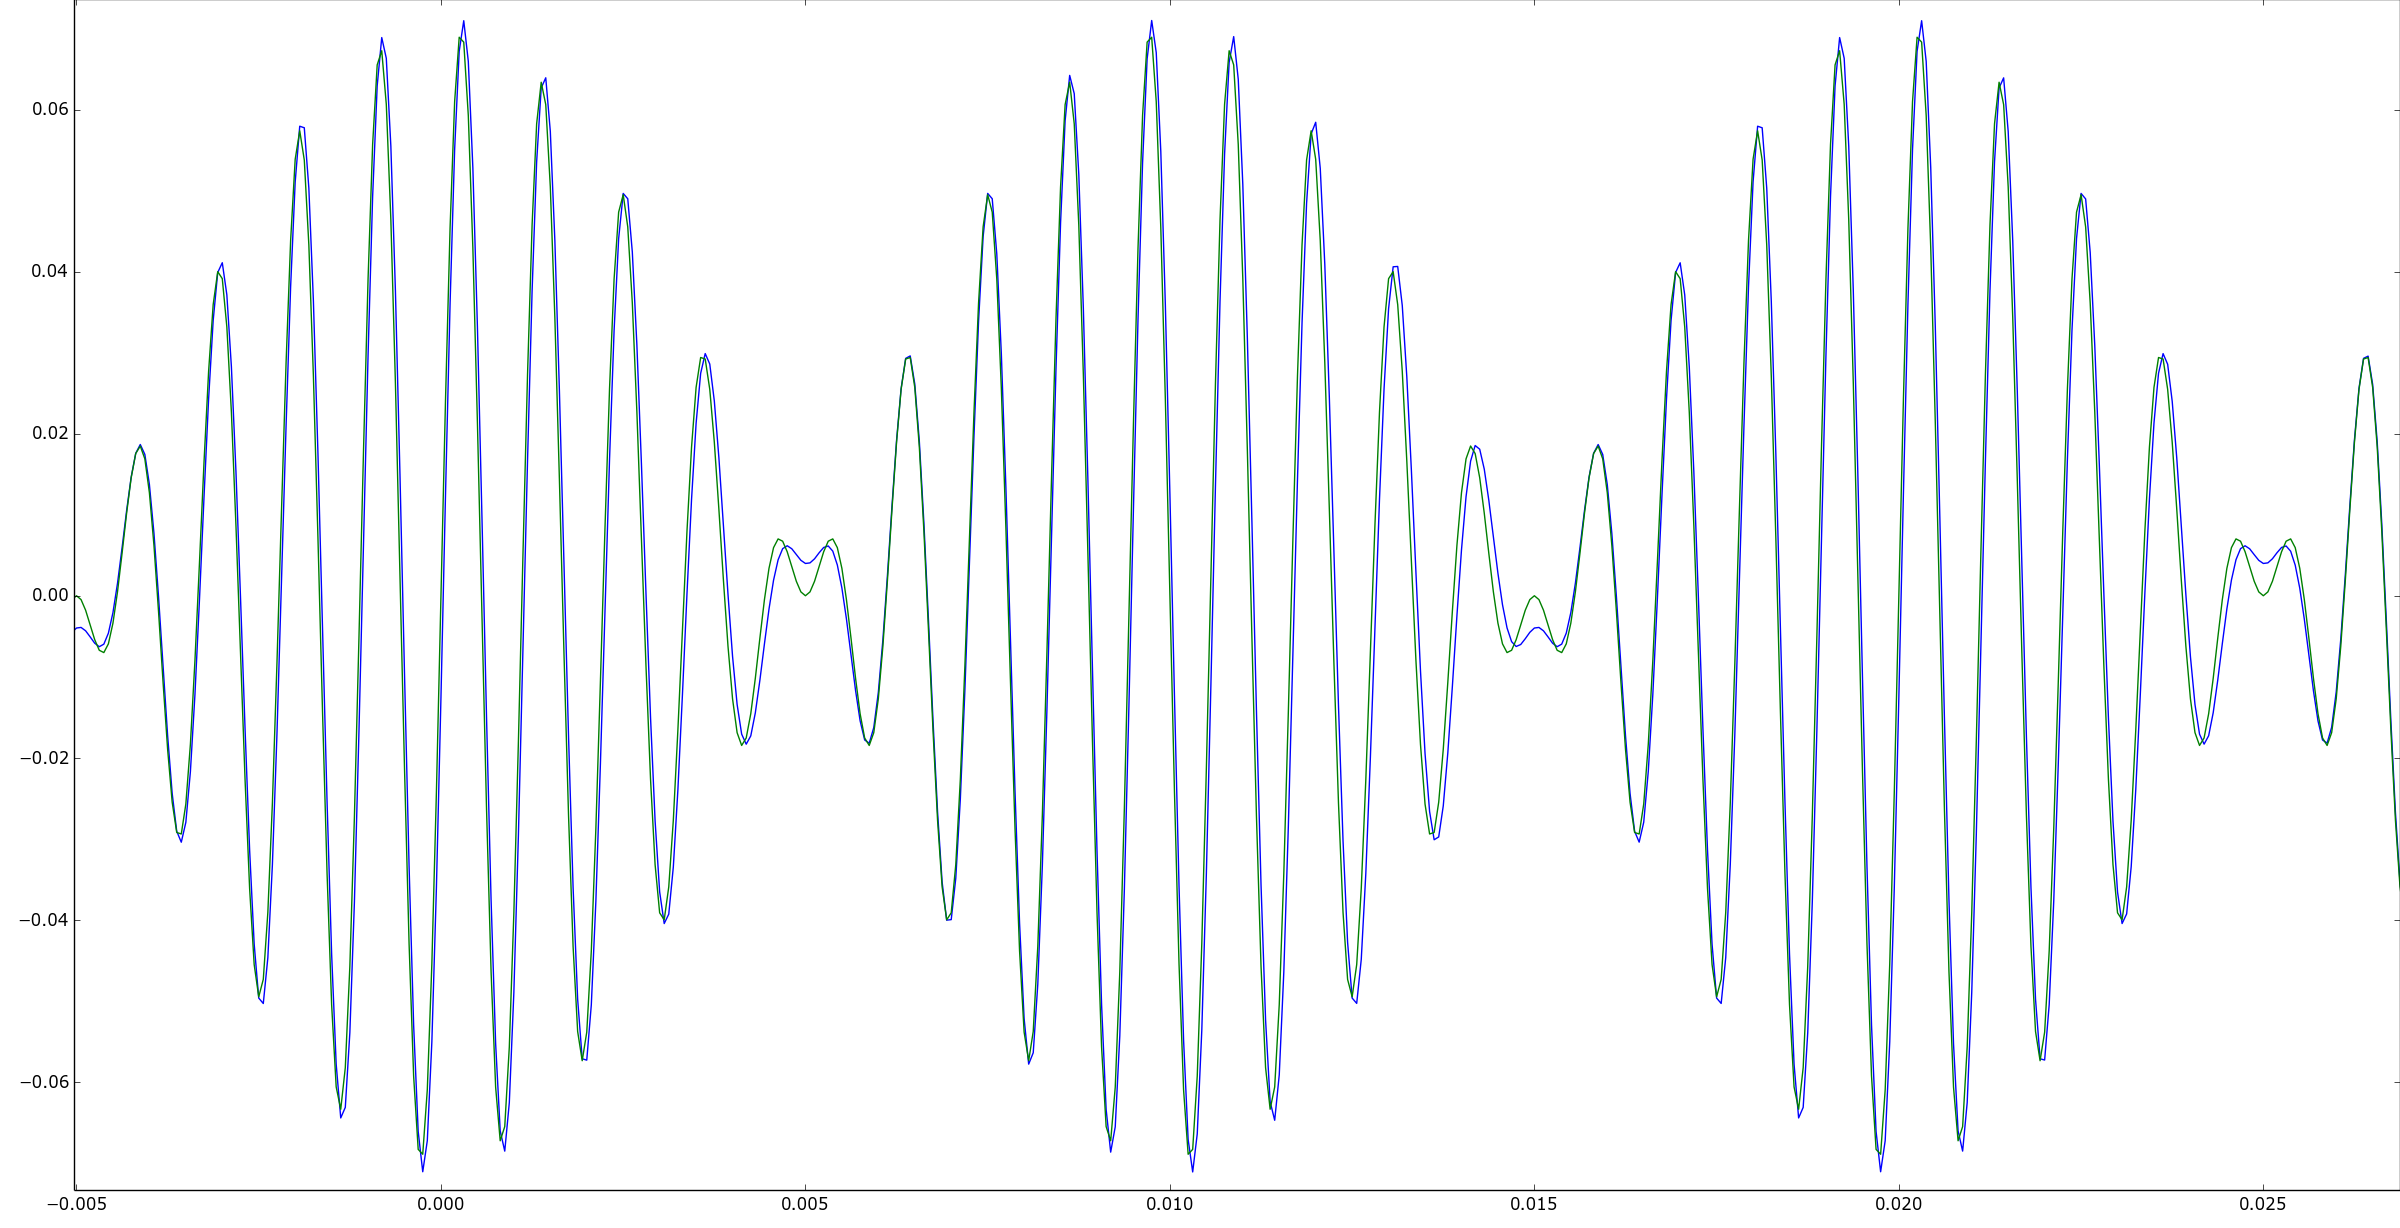
\includegraphics[width = 0.5\linewidth]{prints/sobrepostos_sistema6.png}   
    \caption{Saída aproximada (\textcolor{Green}{a verde}) sobreposta com a saída produzida pelo \(sistema_6\) (\textcolor{Blue}{a azul}).}
    \label{fig:sobrepostos_sistema6}
\end{figure}

Comparando o resultado aproximado obtido com a saída produzida em resposta ao sinal \textit{p} pelo \(sistema_6\), observou-se um resultado bastante satisfatório, dado que as medições do período são as mesmas. As pequenas diferenças entre os gráficos podem ser explicadas pelas aproximações razoáveis efetuadas (com o intuito de simplificar cálculos e manter o documento sucinto) e pelo facto do ambiente laboratorial \textit{Python} ter as suas limitações inerentes (um bom exemplo é a \(\mathbb{R}e\{\mathcal{P}(j\omega)\} \neq 0\), que foi interpretado como uma impureza/ruído).

Concluí-se então que, como esperado, a saída do filtro é de facto uma sinusóide com amplitude que varia no tempo, sendo a \textbf{filtragem do sinal \(p\) através do passa-banda:} \(y(t) \approx k \cdot \cos (2\pi \cdot 50 \cdot t) \cdot \sin (2 \pi \cdot 900 \cdot t)\text{,}\ k \in \mathbb{R}^{+}\). O valor aproximado das frequências, é portanto, \(50\ Hz\ \text{(frequência moduladora) e}\ 900\ Hz\) (frequência local), que correspondem aos valores obtidos experimentalmente.
%}}

\clearpage

\subsection{\bf{Amostragem}}
\label{subsec:amostragem}
%------------------------------------------------------%
\subsubsection{(R9) Amostragem}
\label{subsubsec:R9}
\textbf{Explique como é que o espectro que obteve para o sinal \(y_{c1}\) resultou do de \(x_{c1}\) através dos processos de amostragem e reconstrução de sinais.}
\paragraph{Resposta:} %{{
Comecemos por analisar o sinal \(x_{c1}\). Por observação direta do gráfico visível na \hyperref[fig:xc1]{Fig. 21}, concluí-se que o sinal é real e ímpar pelo que, a sua Transformada de Fourier é puramente imaginária\footnotemark[8].

\begin{figure}[ht]
    \centering
    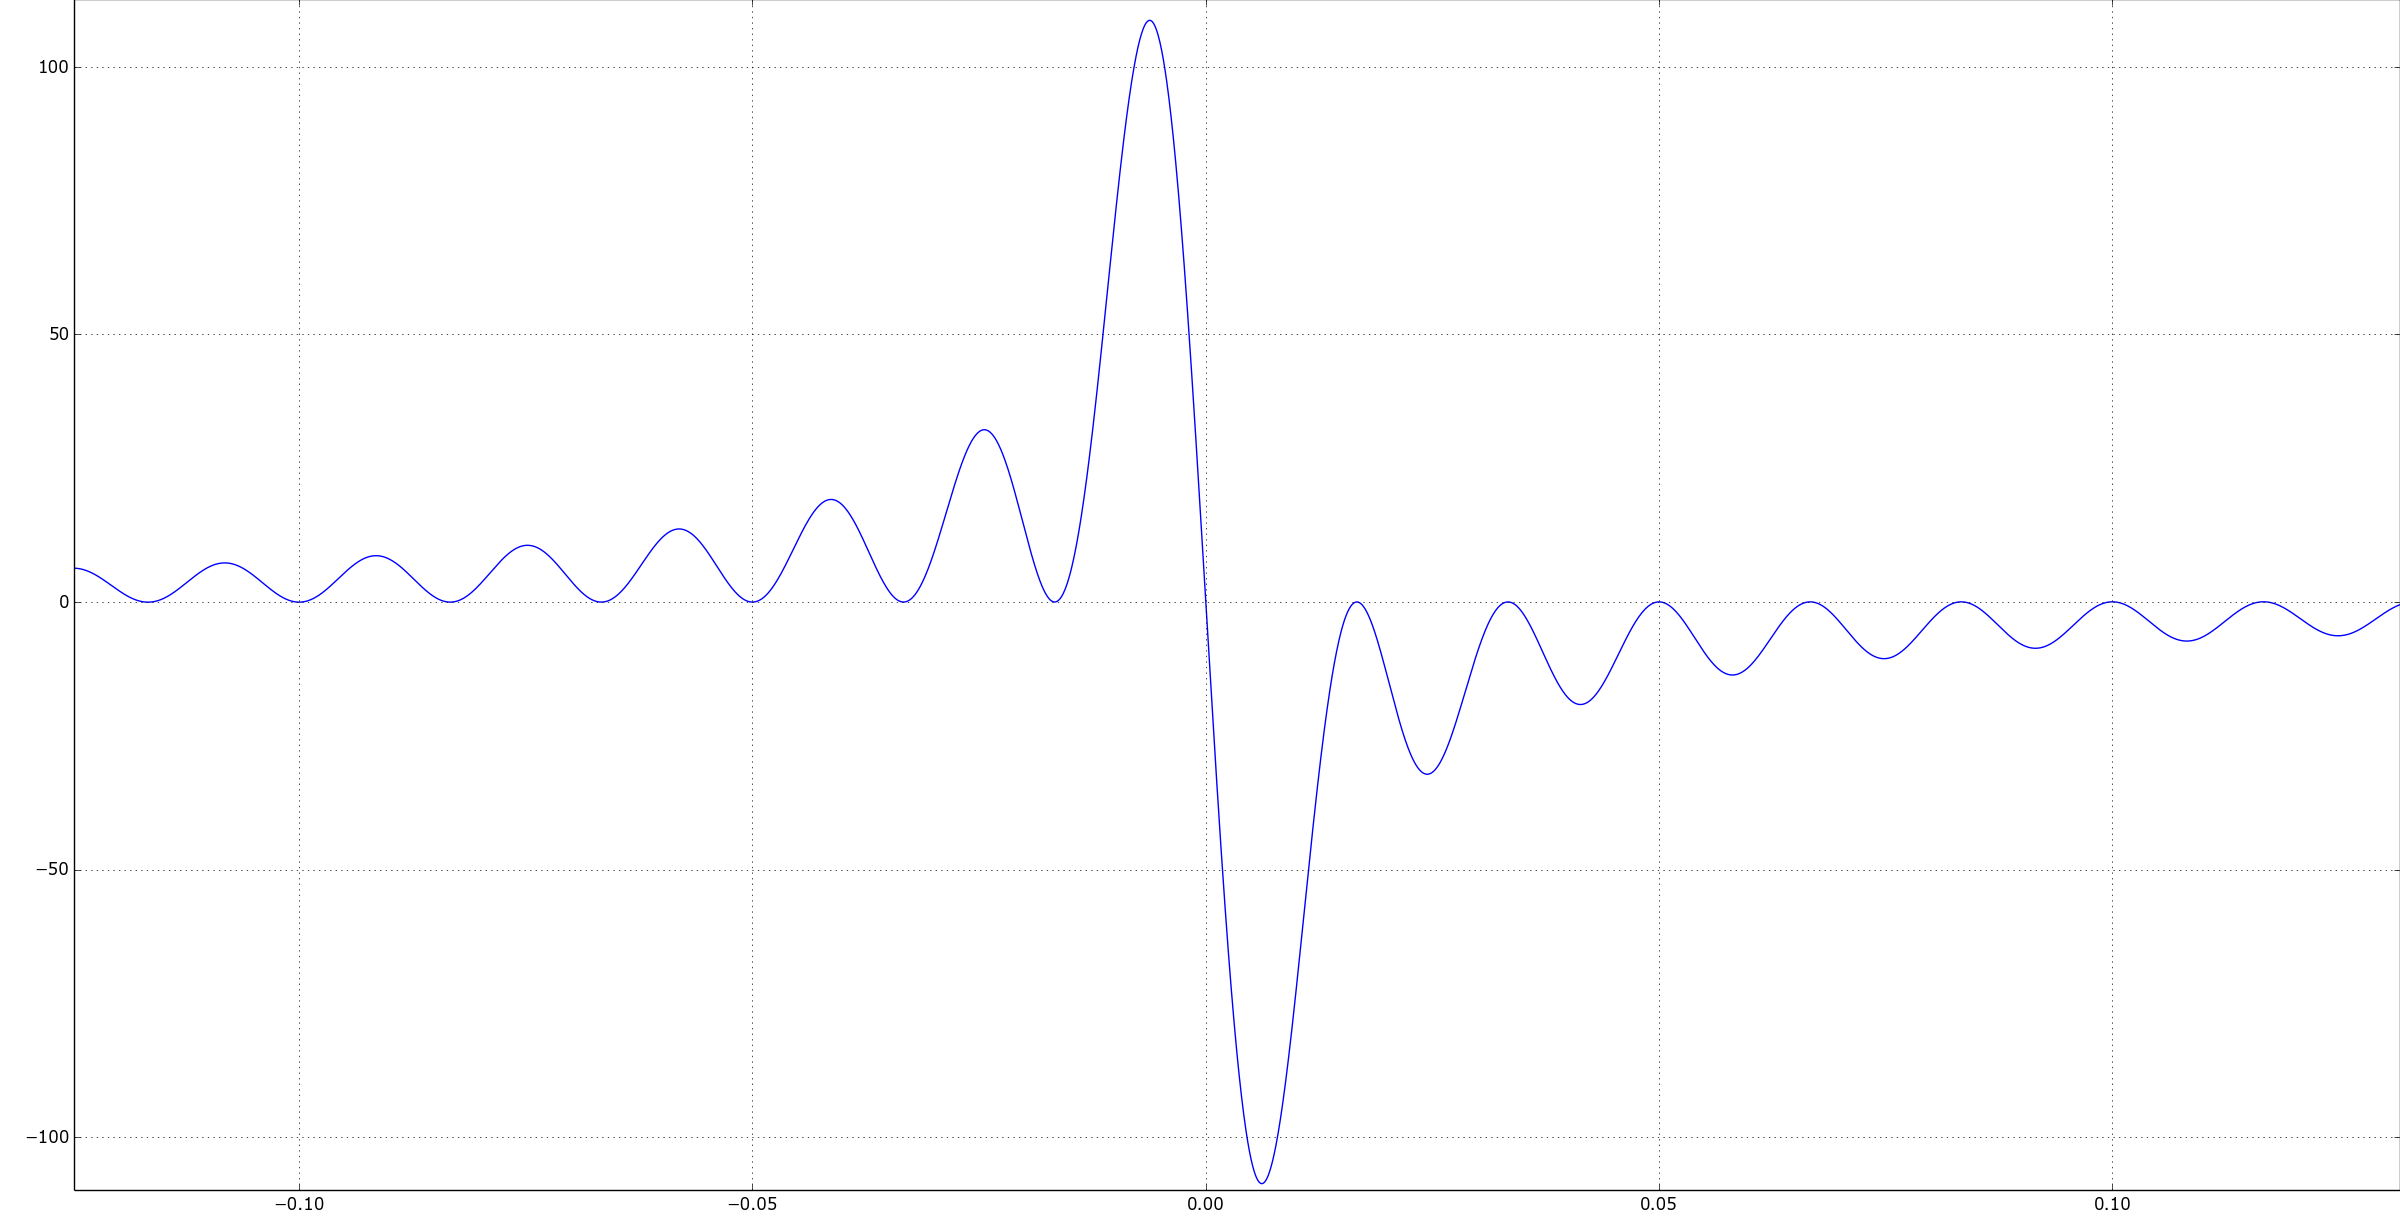
\includegraphics[width = 0.5\linewidth]{prints/xc1.png}   
    \caption{Sinal \(x_{c1}\) no domínio do tempo.}
    \label{fig:xc1}
\end{figure}

\begin{figure}[H] 
    \begin{subfigure}[b]{0.5\linewidth}
        \centering
        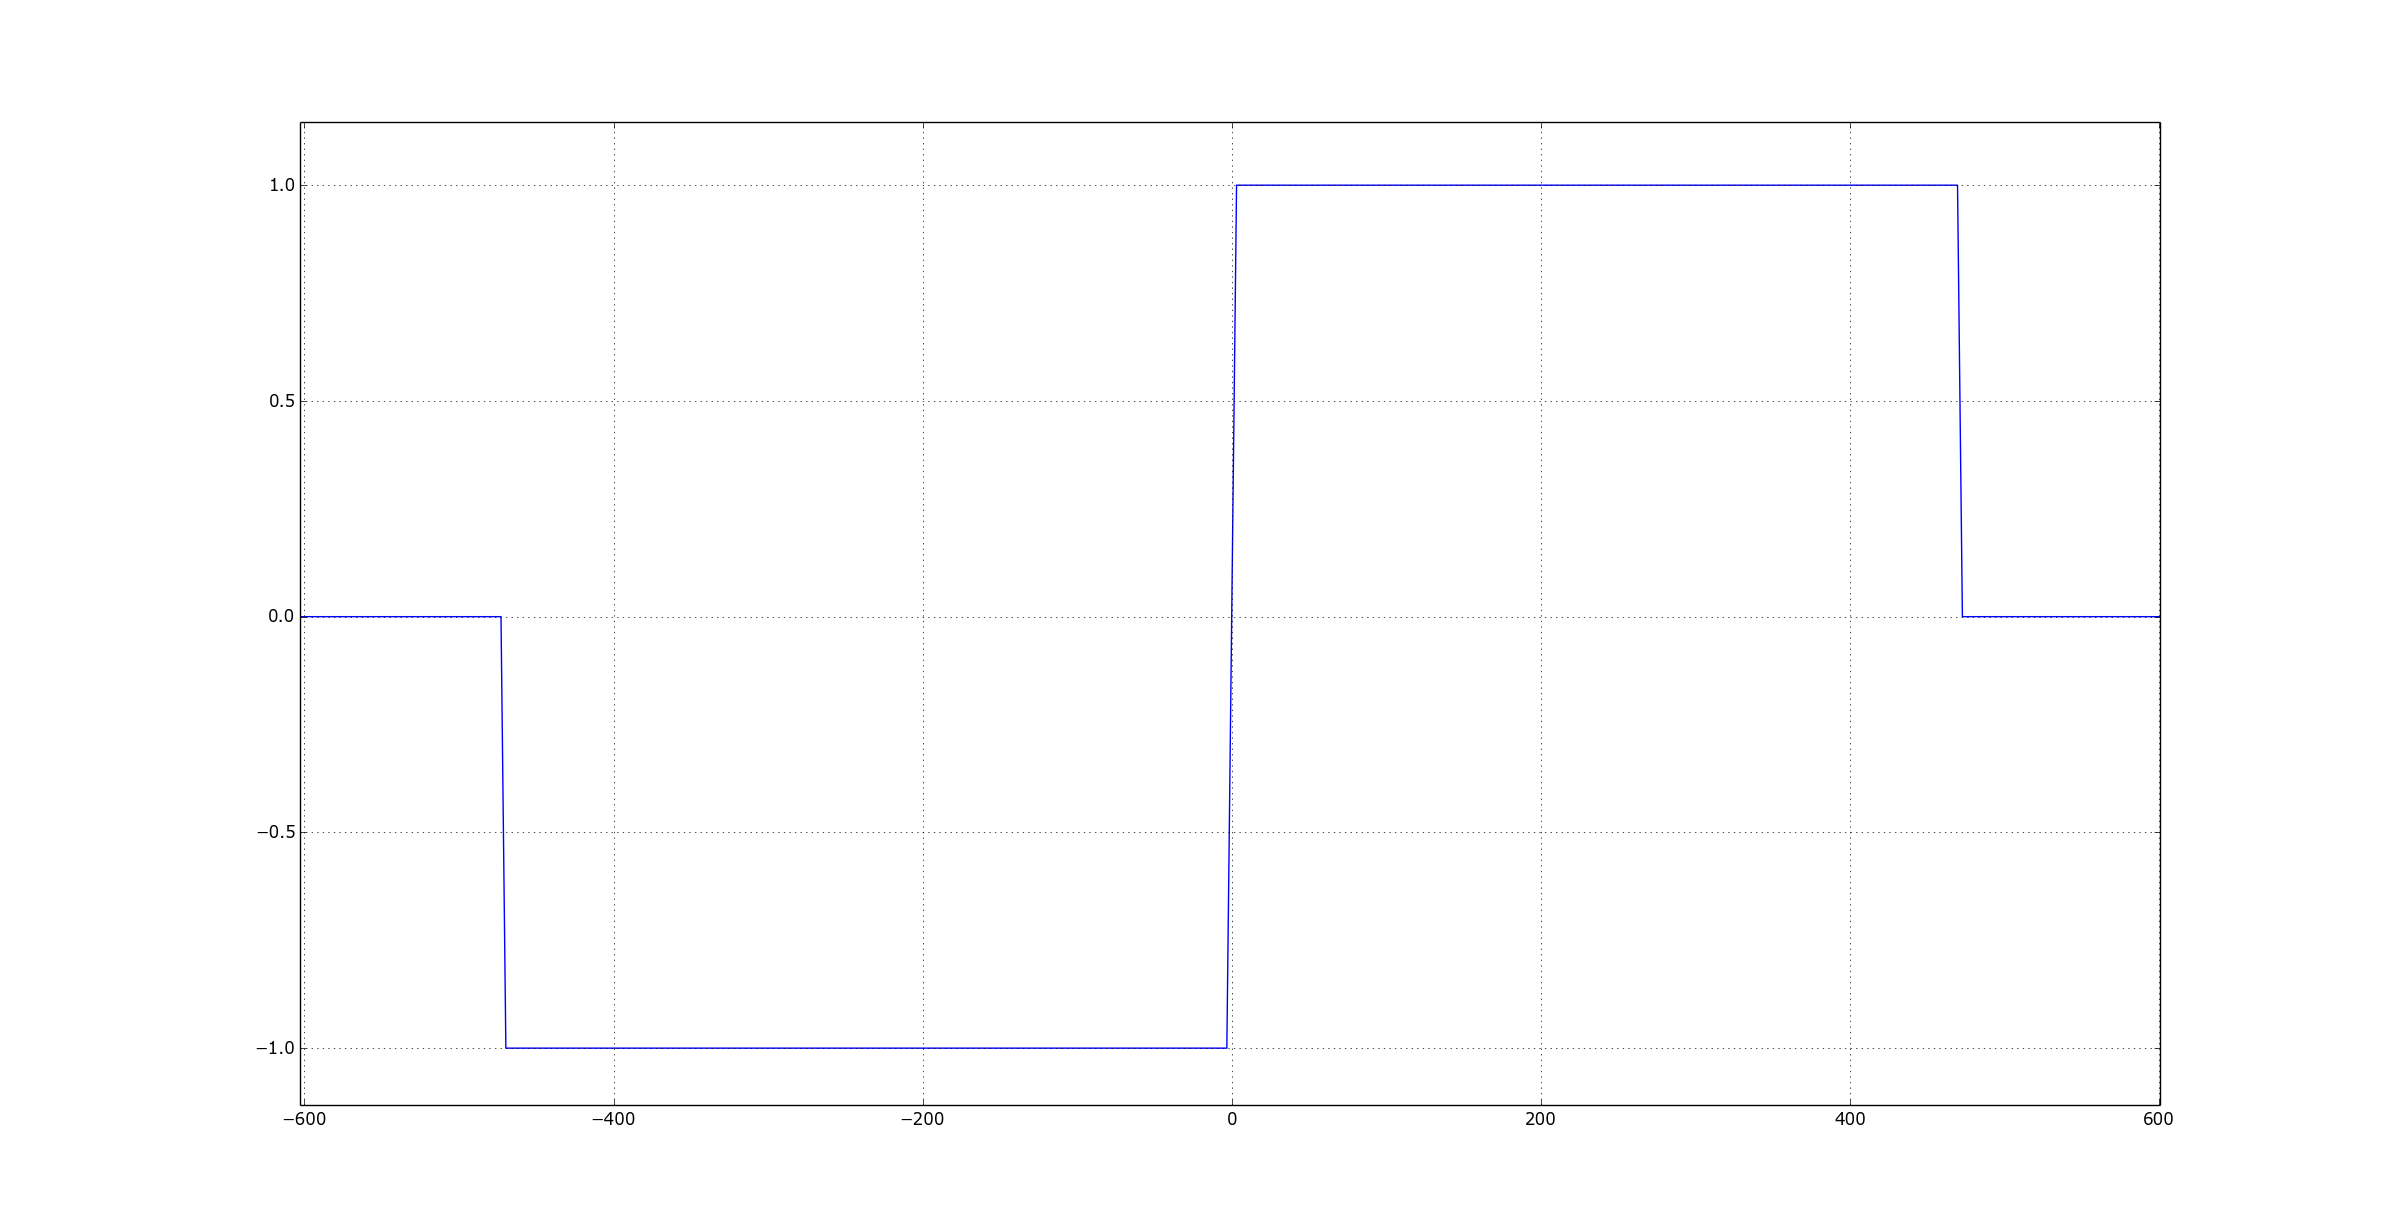
\includegraphics[width=1\linewidth]{prints/imag_XC1.png}
        \caption{\(\mathbb{I}m\{\mathcal{X}_{c1}(j\omega)\}\).} 
        \label{fig:imag_XC1} 
        %%\vspace{4ex}
    \end{subfigure}%% 
    \begin{subfigure}[b]{0.5\linewidth}
        \centering
        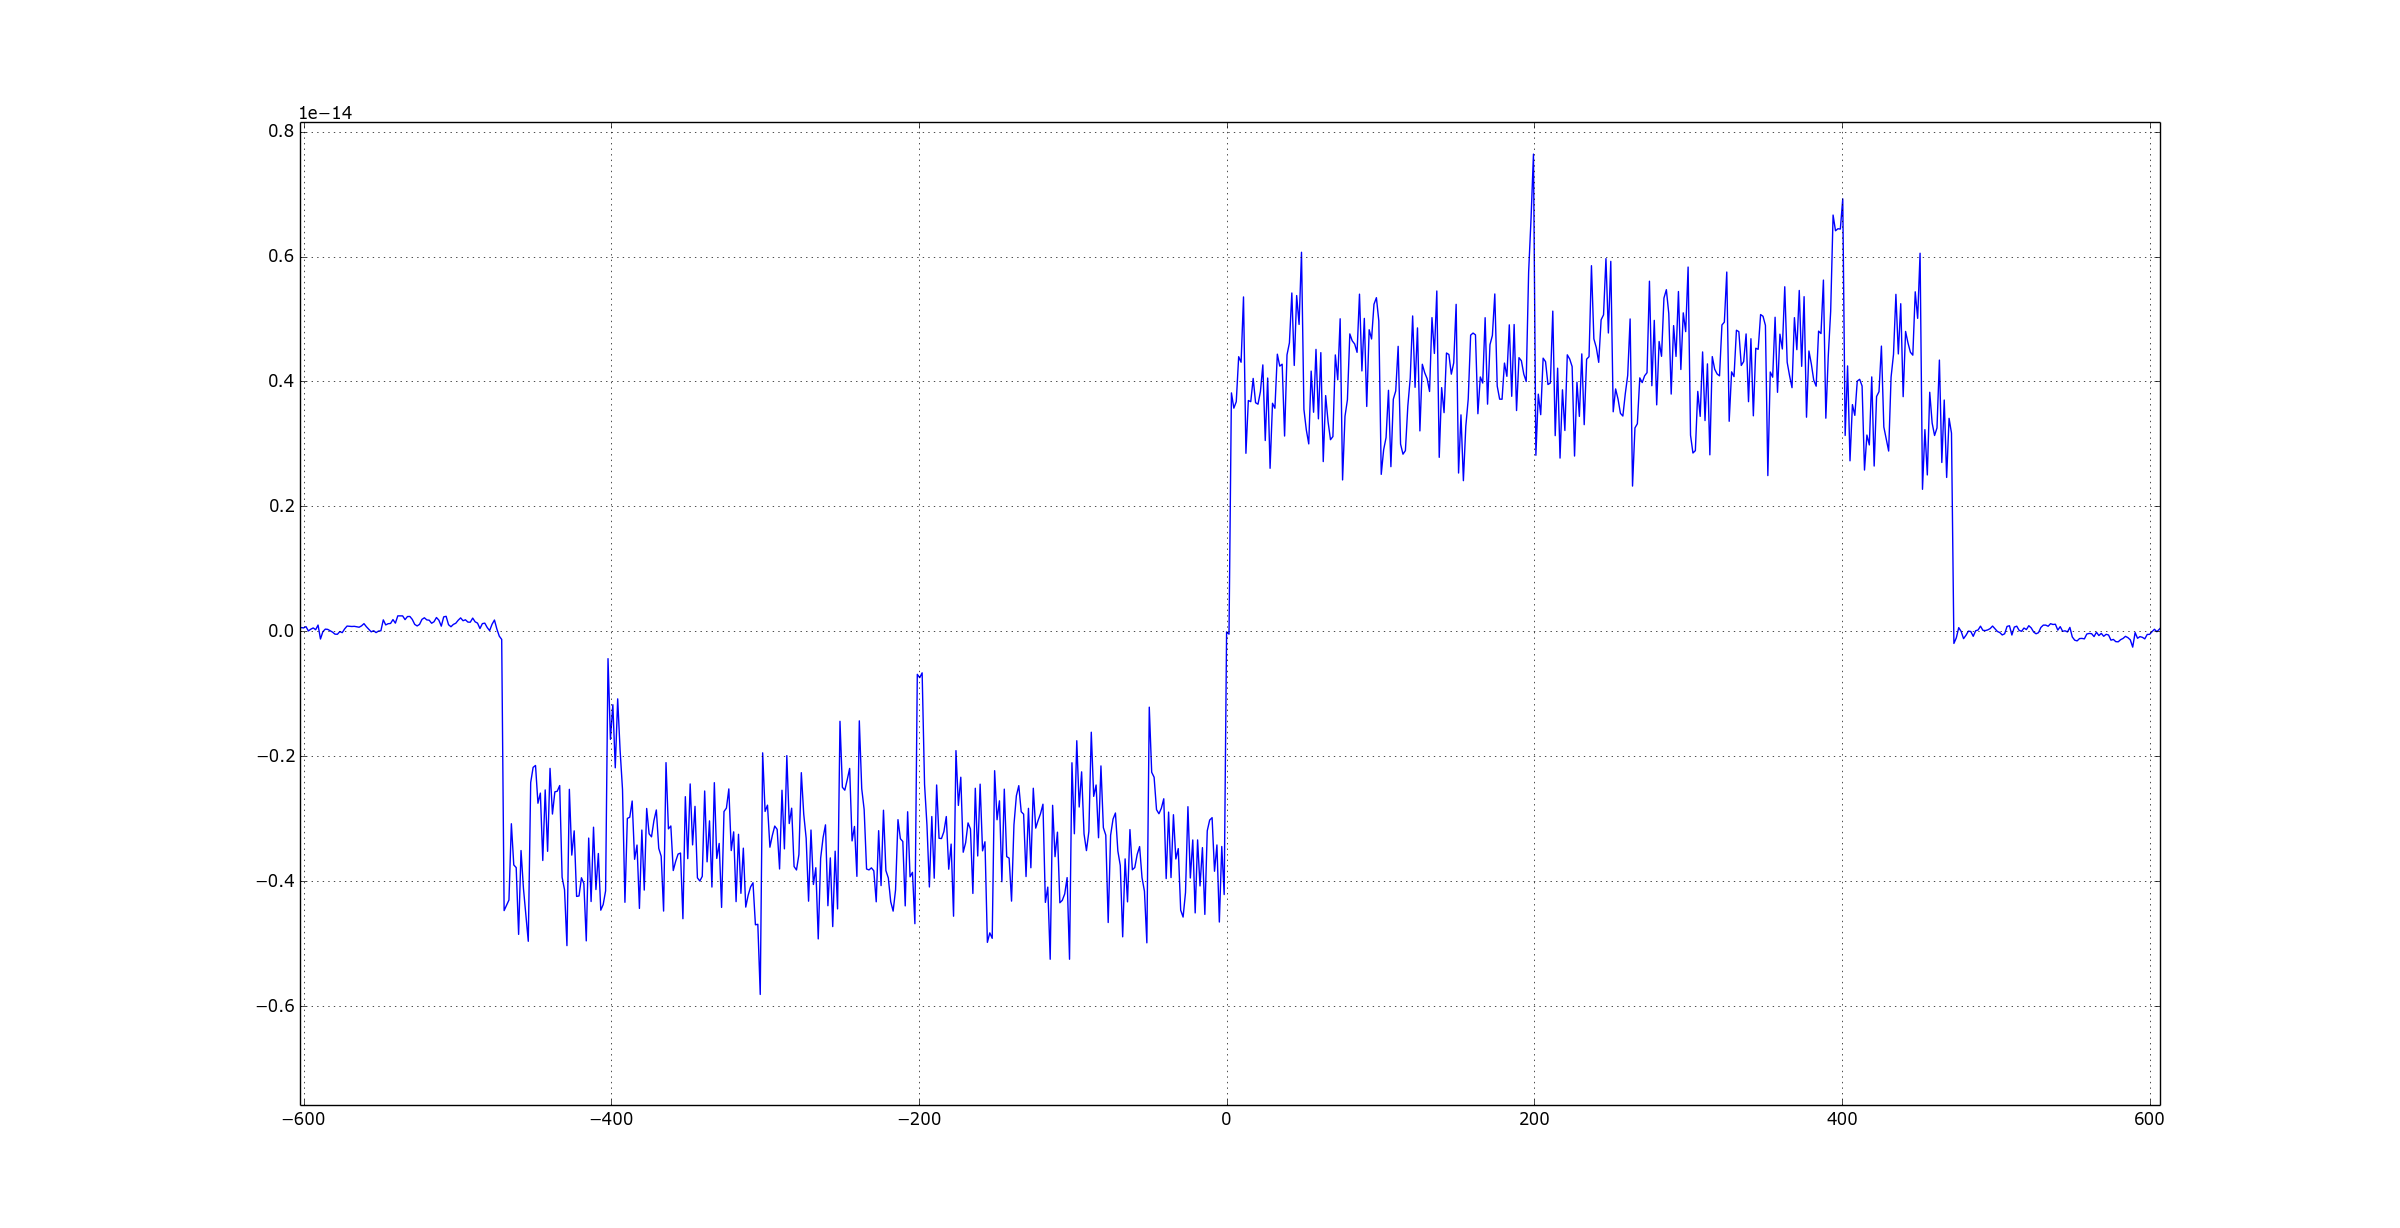
\includegraphics[width=1\linewidth]{prints/real_XC1.png} 
        \caption{\(\mathbb{R}e\{\mathcal{X}_{c1}(j\omega)\}\)} 
        \label{fig:real_XC1} 
        %%\vspace{4ex}
    \end{subfigure} 
    \caption{Visualização do espectro de \(x_{c1}\).}
    \label{fig:multiplas_8}
\end{figure}

De seguida, pela observação do espectro de \(x_{c1}\), \(\mathcal{X}_{c1}(j\omega)\), (apenas considerada a parte imaginária do espectro) concluí-se que a banda máxima do sinal é \(\omega_M = 470\ \text{rad}\ s^{-1}\). 
Uma vez que o período de amostragem é \(T = 0.01\ \text{s}\), a frequência de amostragem é então \(\omega_S = \frac{2\pi}{T} = 628\ \text{rad}\ s^{-1}\). Note-se que é inferior à frequência de Nyquist \(\omega_N = 2\ \omega_M = 940\ \text{rad}\ s^{-1}\), pelo que \textbf{não nos encontramos nas condições do Teorema da Amostragem}, não sendo garantida a recuperação do sinal \(x_{c1}\) através da aplicação de um filtro passa-baixo com ganho \(T\) no sinal:

\[x_p(t) = \sum \limits_{n = -\infty}^{\mbox{}+\infty} x_{c1}(nT) \delta (t - nT)\]

\footnotetext[8]{É facilmente retificado ao observar a parte real do espectro de \(x_{c1}\) que se tratam de ruídos presentes no sinal, como explícito na \hyperref[fig:real_XC1]{Fig. 22 (b)}.}

\clearpage

Para uma visualização mais clara do processo de amostragem e de reconstrução do sinal, é proveitoso observar o sinal \(x_p(t)\) em frequência:

\[\mathcal{X}_p(j\omega)=\sum \limits_{k = -\infty}^{\mbox{}+\infty} \frac{1}{T} \mathcal{X}_{c1}(j(\omega-k \cdot \omega_S))\text{,}\] 

Uma vez que \(\omega_S\ -\ \omega_M = 158\ \text{rad}\ s^{-1}\), ocorre inevitavelmente uma sobreposição de réplicas, tal como é possível observar na figura \hyperref[fig:XP_replicas]{Fig. 23}. 

%\iffalse
\begin{figure}[ht]
    \centering
    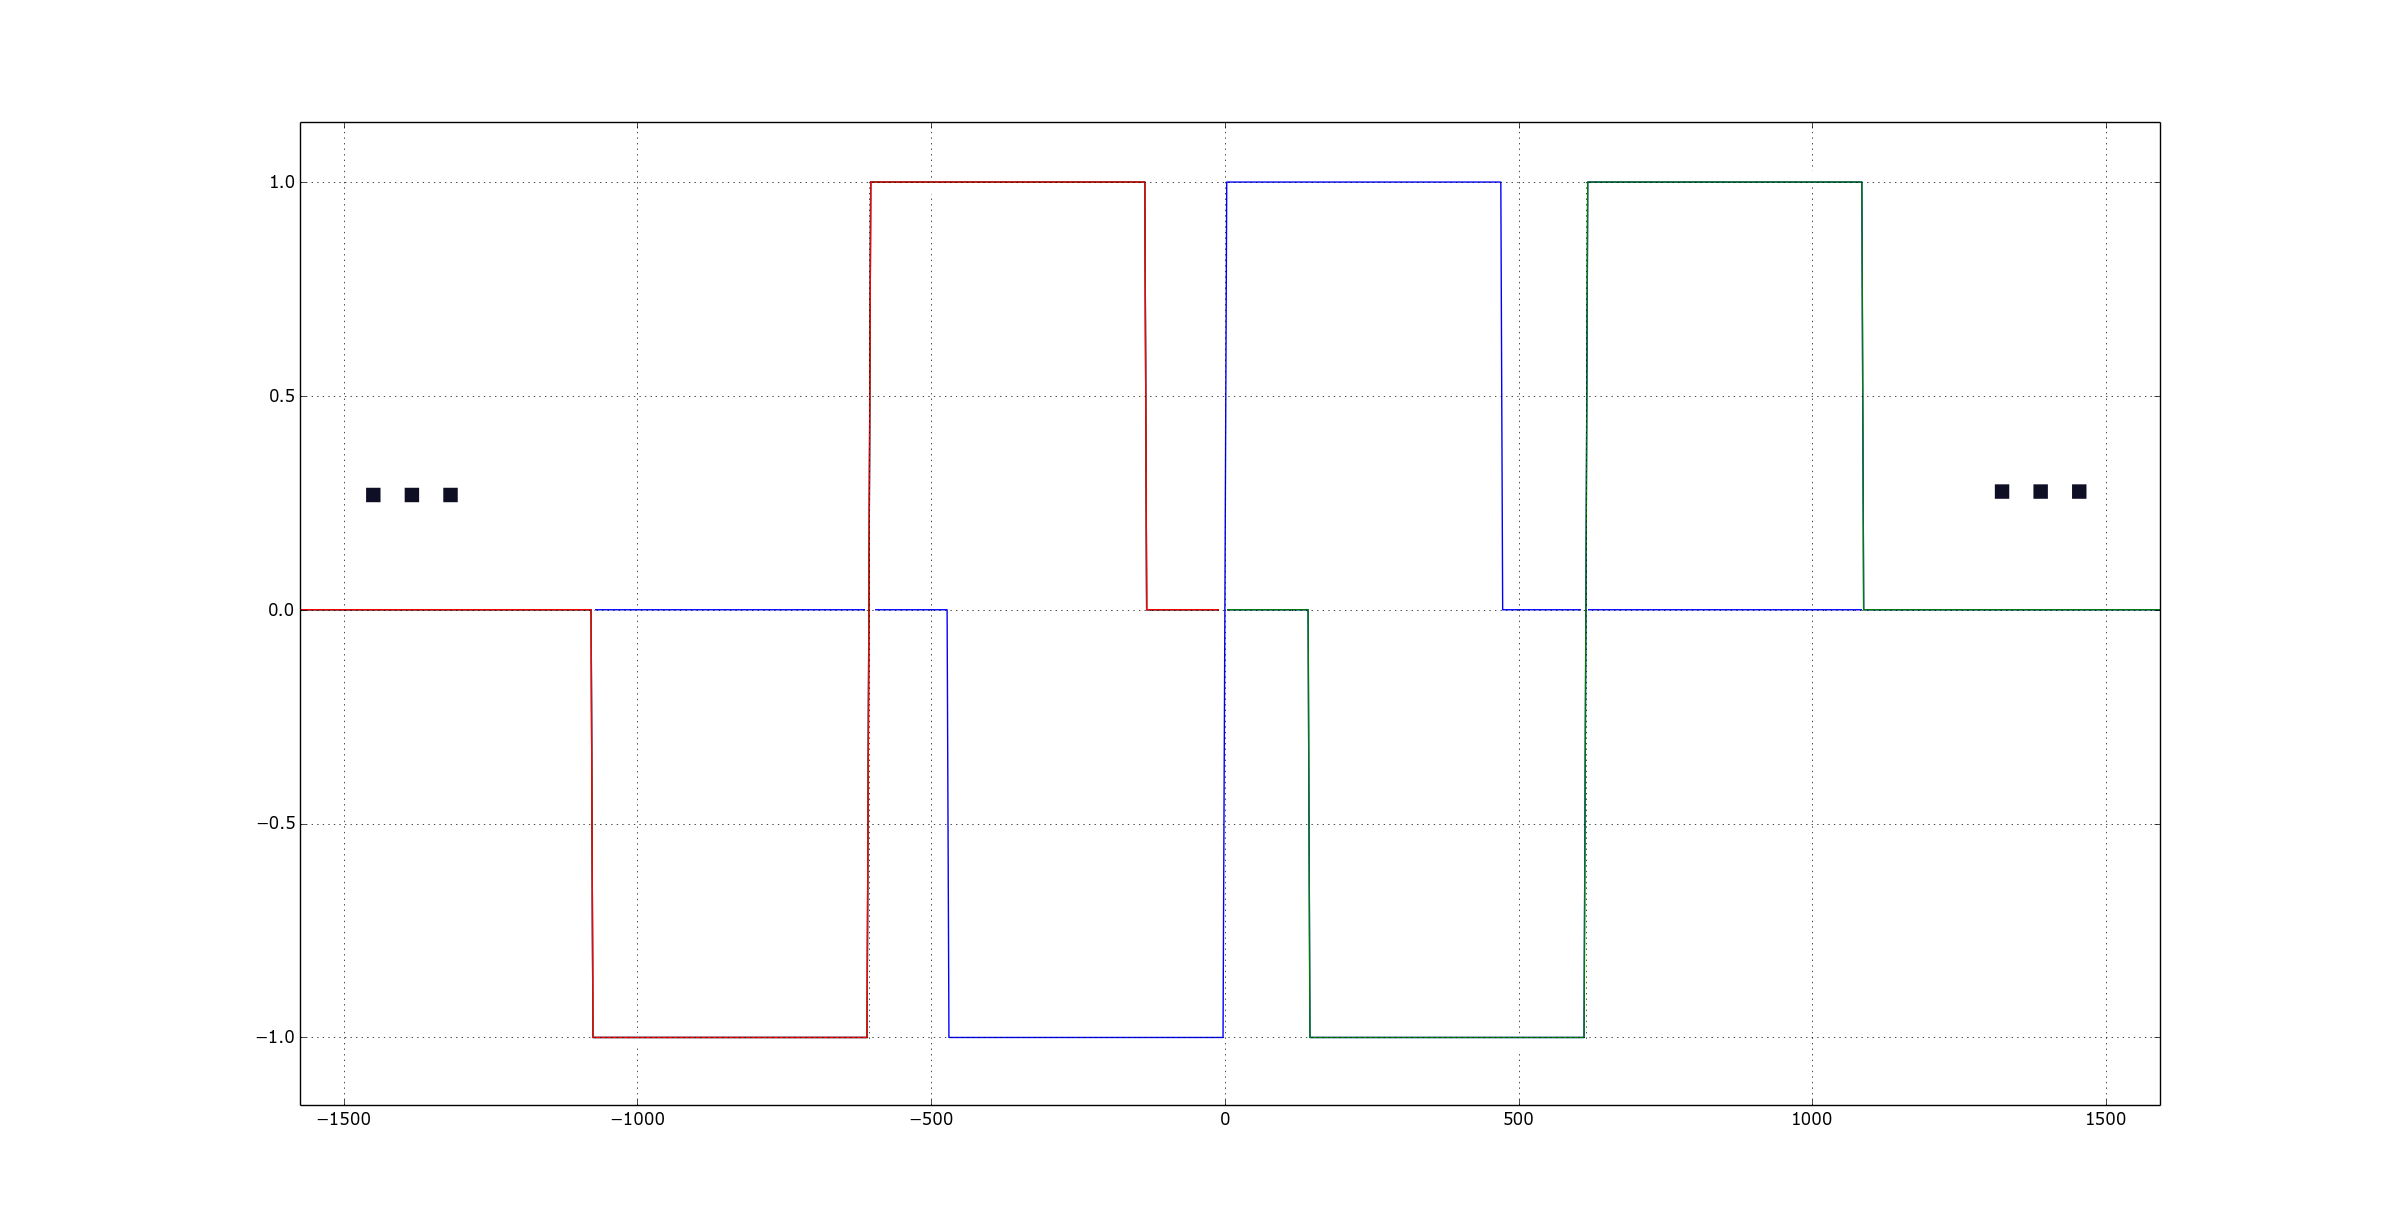
\includegraphics[width = 0.5\linewidth]{prints/XP_replicas.png}   
    \caption{Sobreposição das réplicas de \(\mathcal{X}_{c1}(j\omega)\) deslocadas \(k \cdot \omega_S\).}
    \label{fig:XP_replicas}
\end{figure}
%\fi

Após se somarem as diferentes réplicas o resultado obtido é o da \hyperref[fig:XP_soma]{Fig. 24} , note-se que o sinal ficou reduzido ao pequeno intervalo \(\pm 158\ \text{rad}\ s^{-1}\) em torno de \(k \cdot \omega_S\), \(k \in \mathbb{Z}\).

%\iffalse
\begin{figure}[ht]
    \centering
    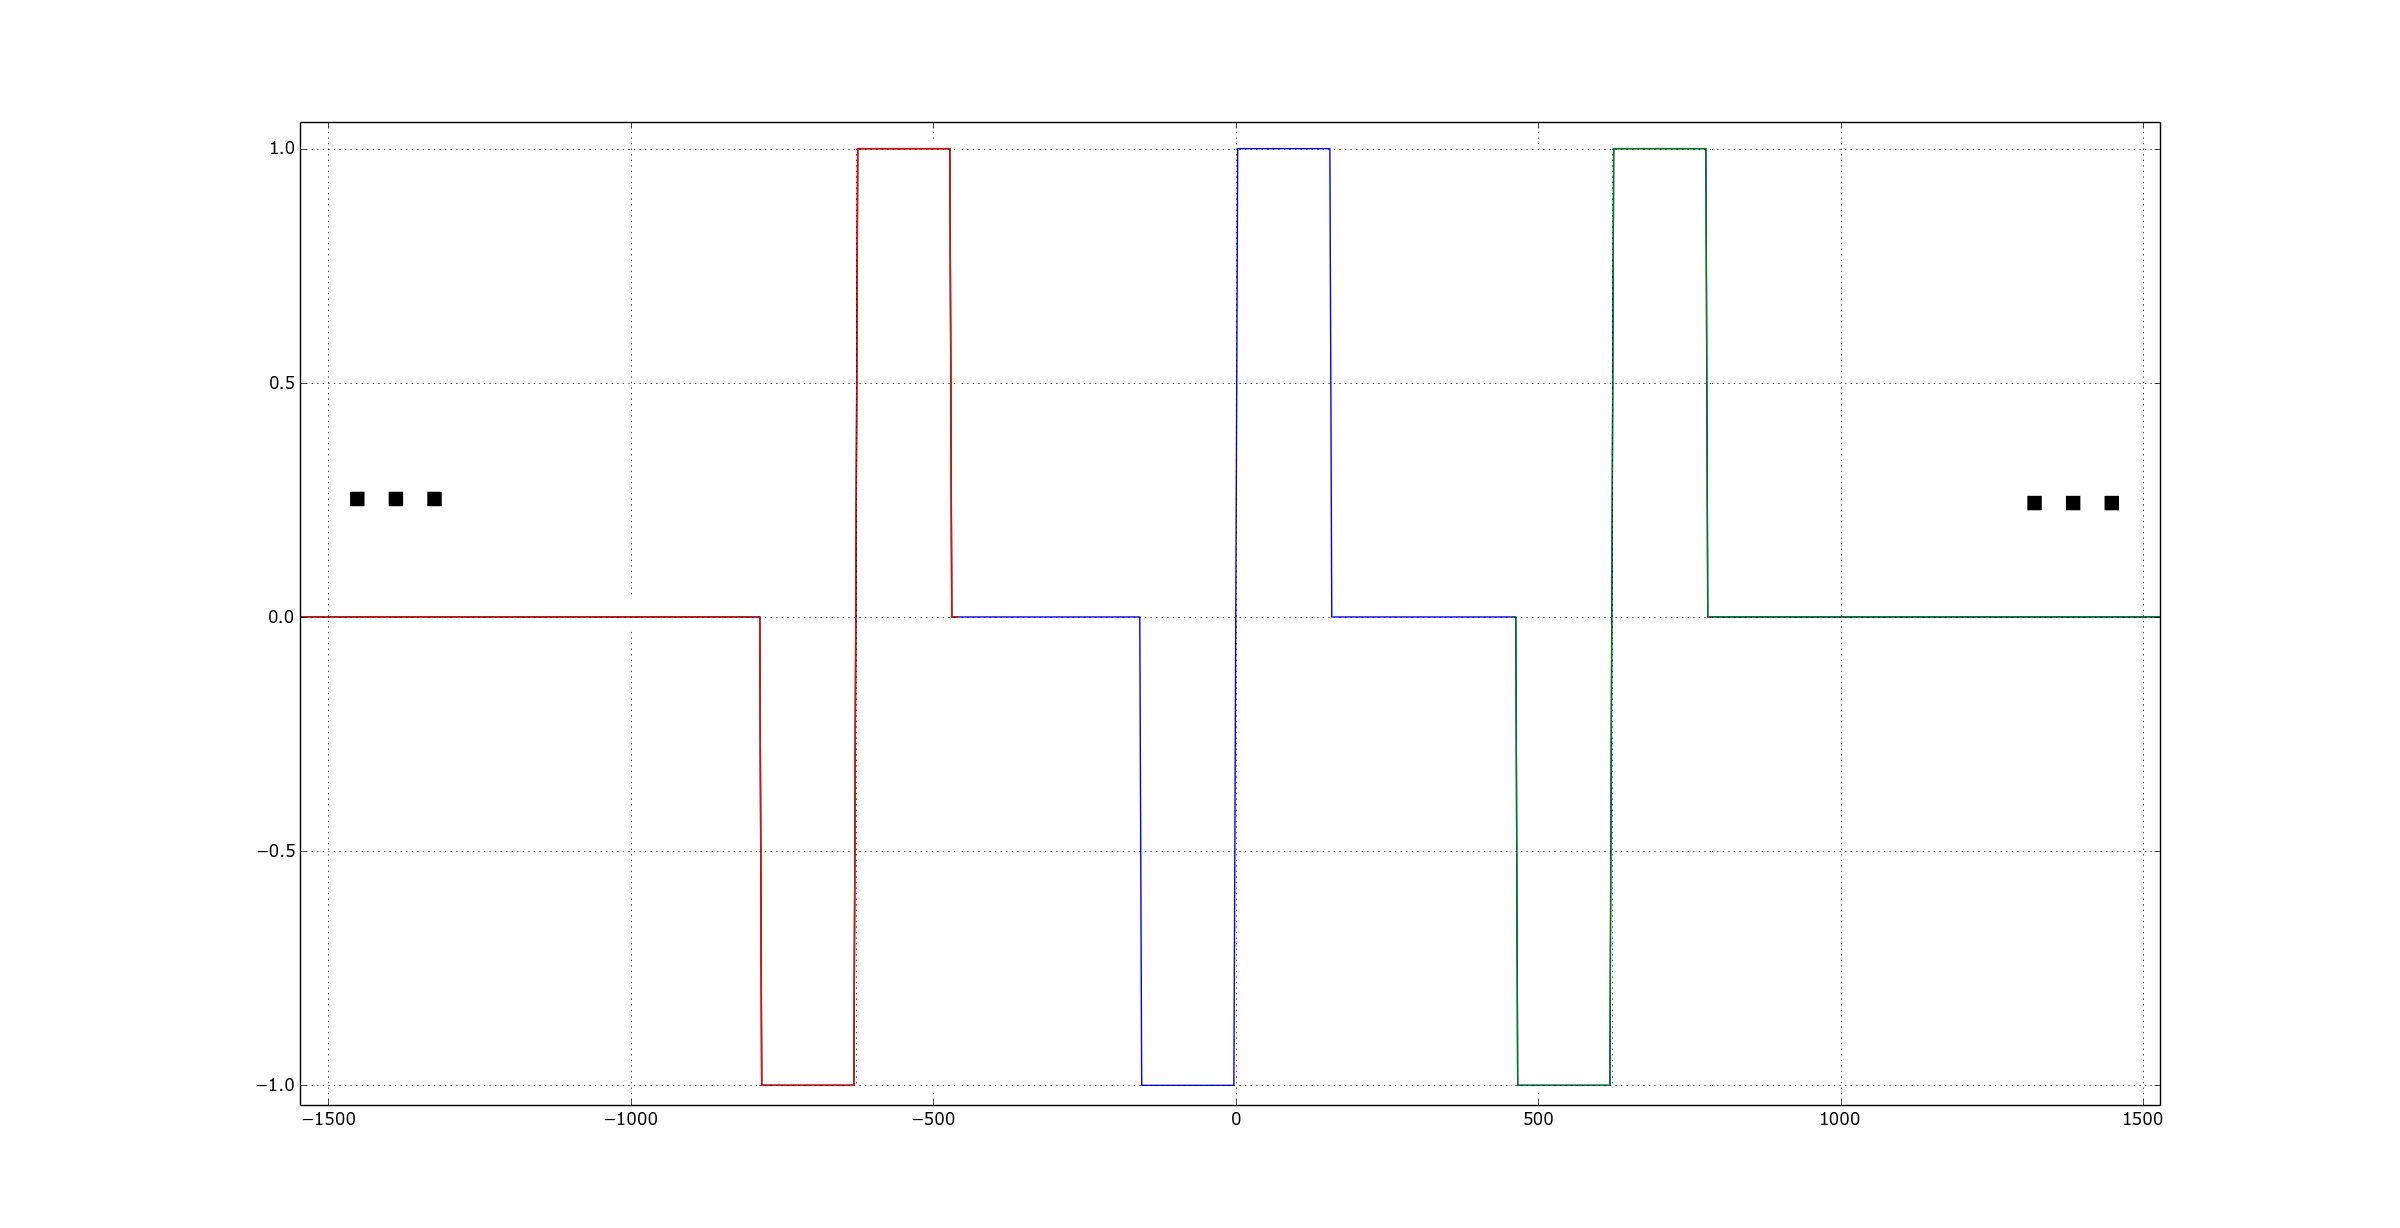
\includegraphics[width = 0.5\linewidth]{prints/XP_soma.png}   
    \caption{Representação gráfica de \(\mathcal{X}_p(j\omega)\).}
    \label{fig:XP_soma}
\end{figure}
%\fi

No processo de reconstrução o sinal passa por um filtro passa-baixo, quase ideal, \(\mathcal{H}_R(j\omega)\) com ganho T e frequência de corte \(\vert \omega_c\vert = \frac{\omega_S}{2} = 314\ \text{rad}\ s^{-1}\). O nosso sinal reconstruído é então \(\mathcal{X}_R(j\omega) = \mathcal{X}_p(j\omega) \cdot \mathcal{H}_R(j\omega)\) tal como representado na \hyperref[fig:YC1]{Fig. 25}. 

\clearpage

%\iffalse
\begin{figure}[ht]
    \centering
    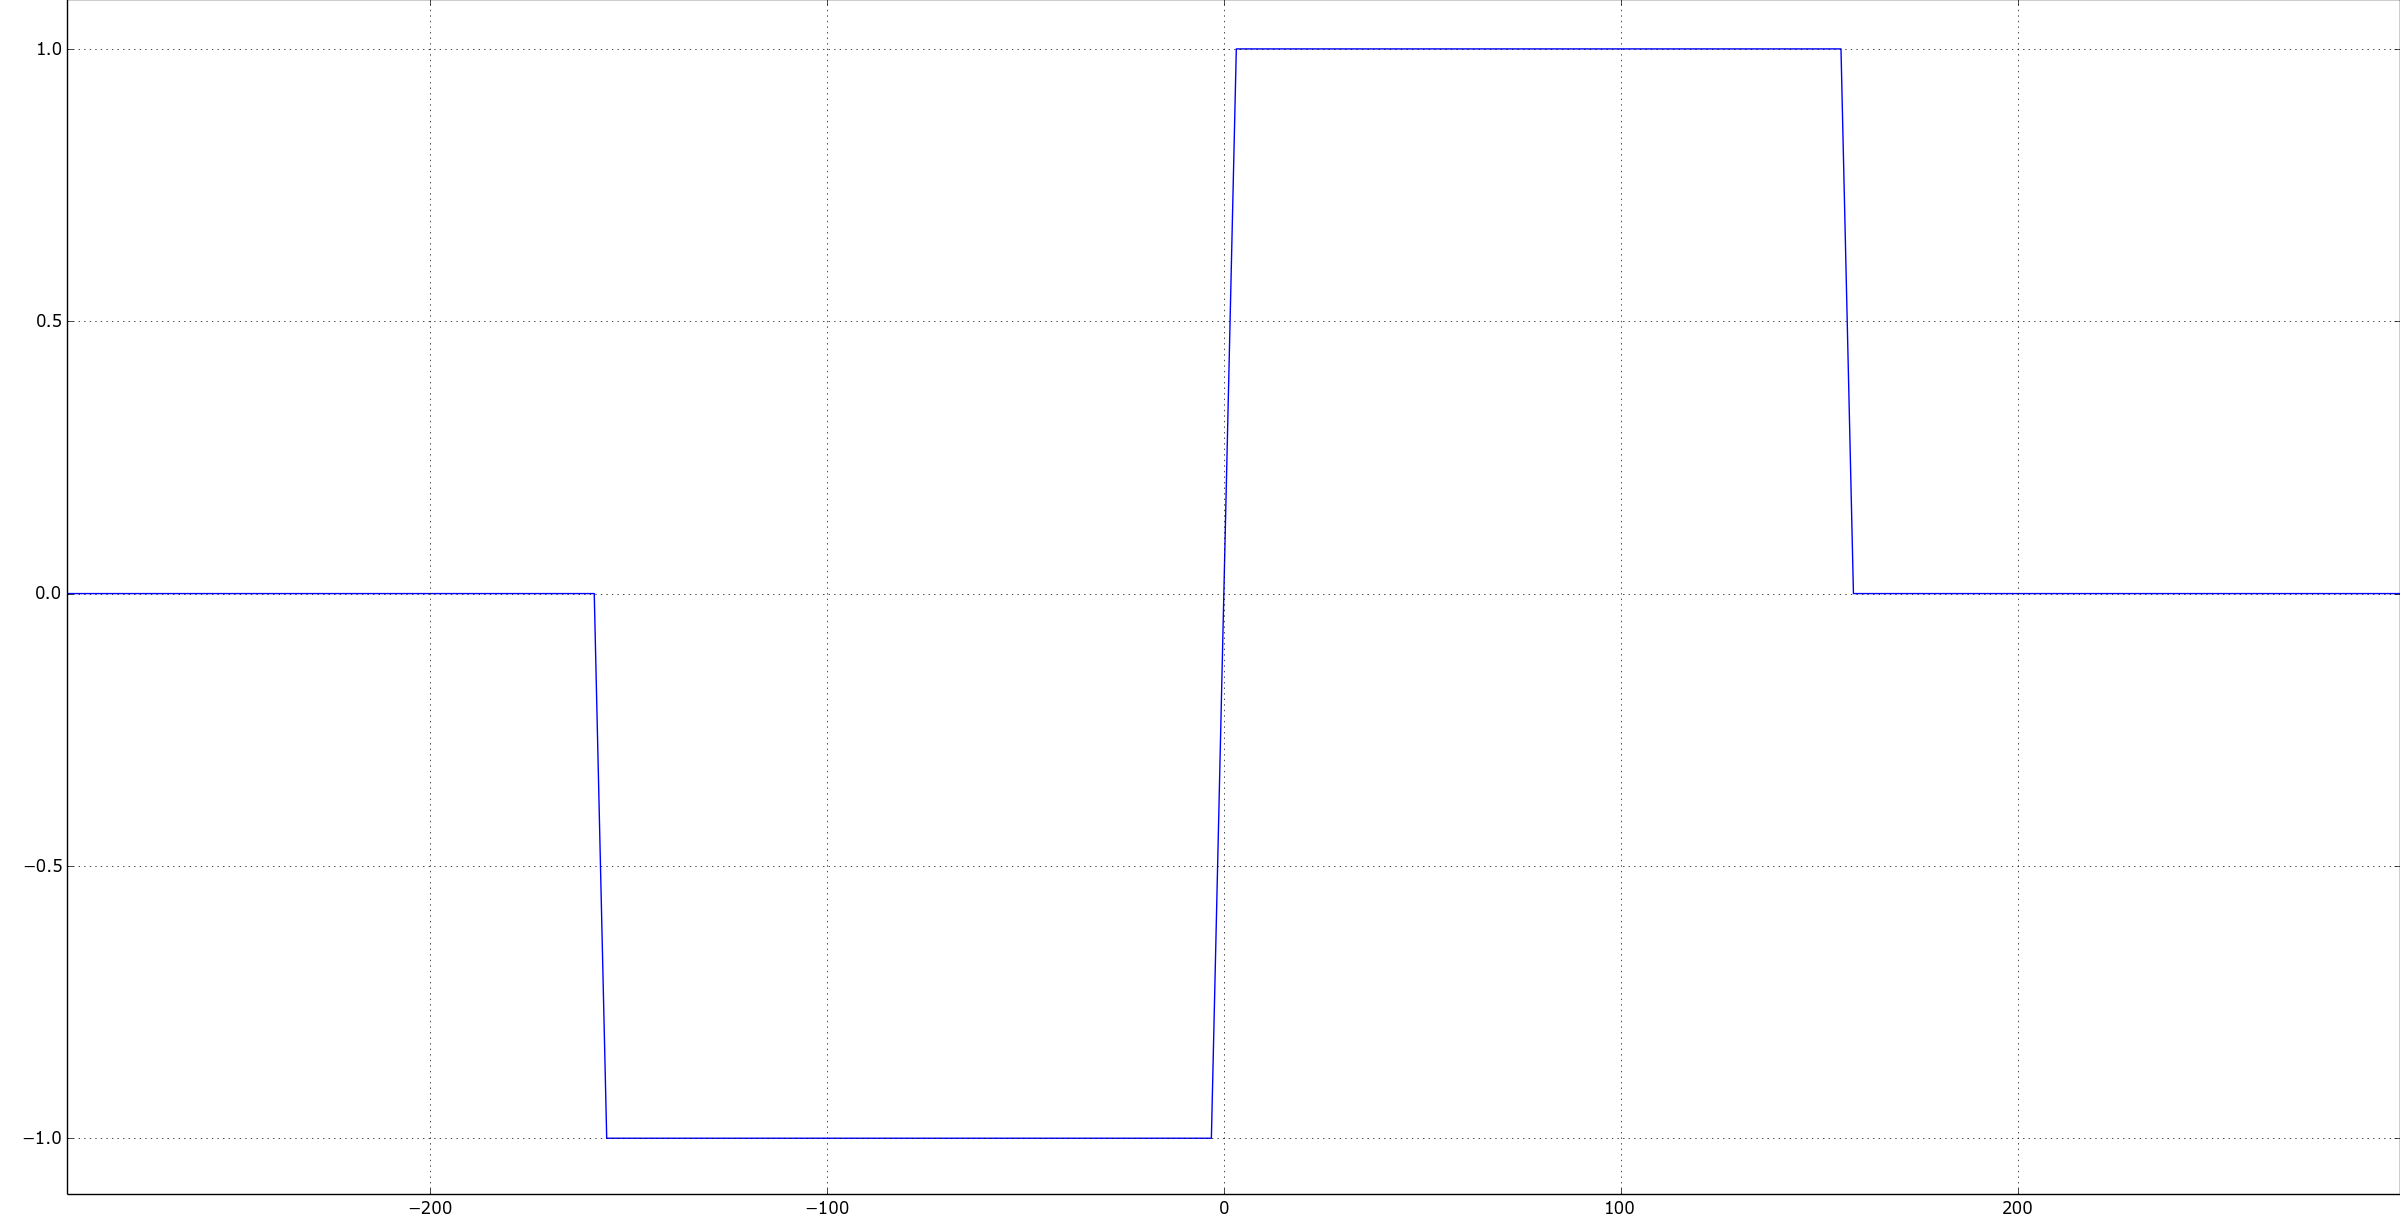
\includegraphics[width = 0.5\linewidth]{prints/YC1.png}   
    \caption{Espectro de \(y_{c1}\), que é obviamente menor do que o de \(x_{c1}\) visivel na \hyperref[fig:imag_XC1]{Fig. 22 (a)} (repare-se que a escala no eixo das abcissas diminuiu).}
    \label{fig:YC1}
\end{figure}
%\fi

Após a observação do sinal \(\mathcal{Y}_{c1}(j\omega)\) obtido experimentalmente, concluímos que corresponde exatamente ao processo formulado teoricamente descrito acima (i.e., \(\mathcal{Y}_{c1}(j\omega)\) corresponde ao \(\mathcal{X}_R(j\omega)\) discutido apenas de forma abstrata), no qual tínhamos concluído que (em frequência) a partir de \(\omega\ =\ \pm158\ \text{rad}\ s^{-1}\) o sinal fica nulo.

%\iffalse
\begin{figure}[ht]
    \centering
    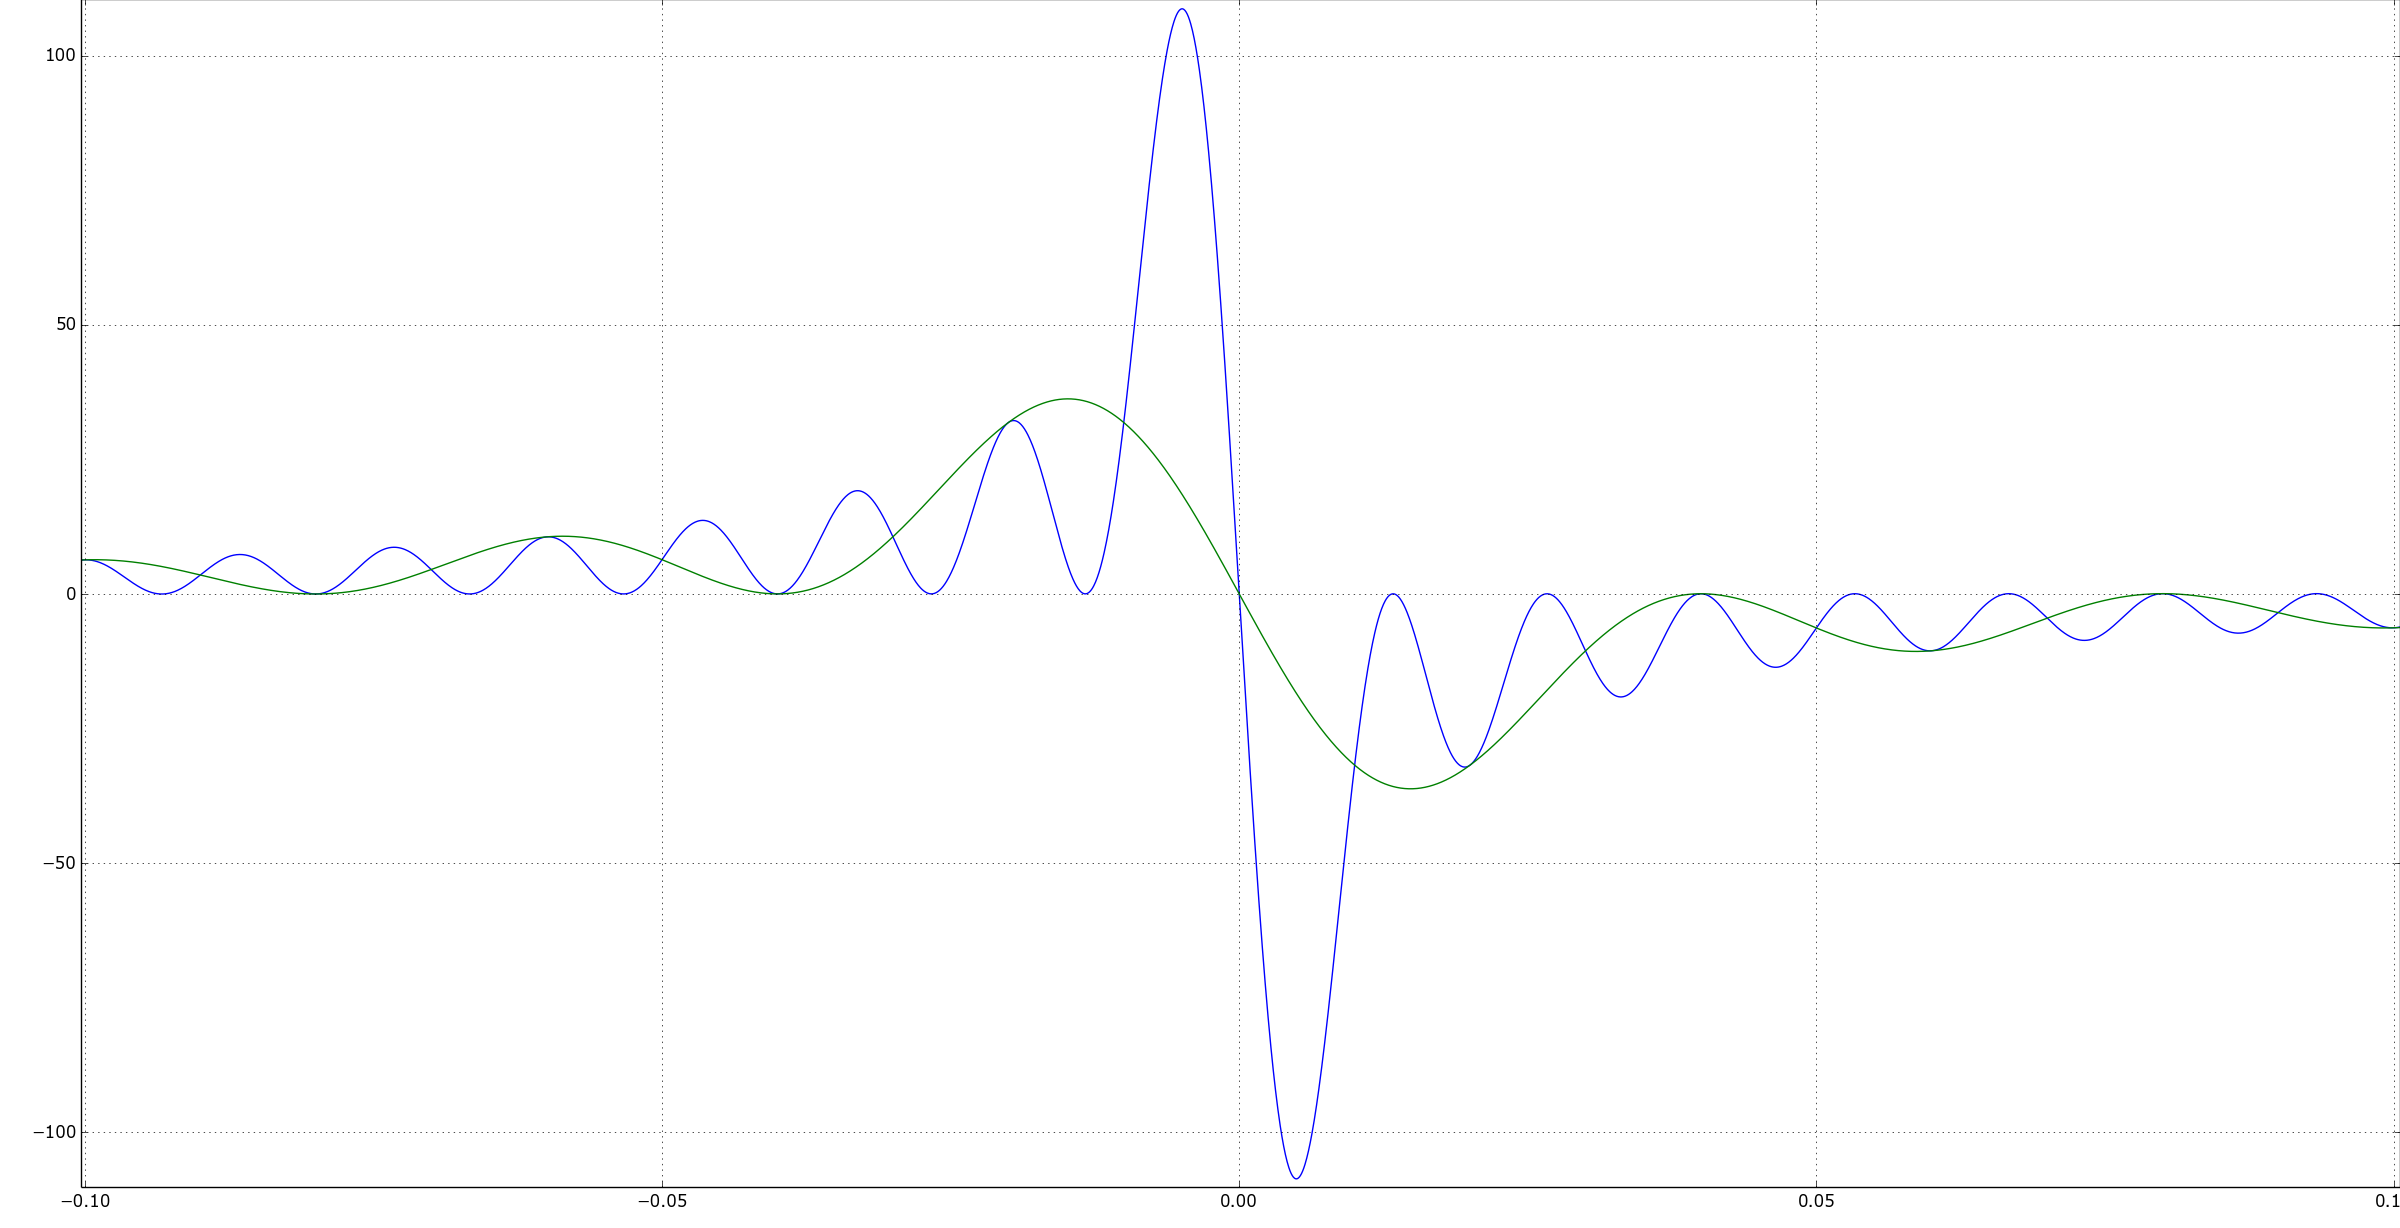
\includegraphics[width = 0.5\linewidth]{prints/yc.png}   
    \caption{\(x_{c1}\), sinal original (\textcolor{Blue}{a azul}) e \(y_{c1}\), sinal reconstruído com \textit{aliasing} (\textcolor{Green}{a verde}).}
    \label{fig:yc}
\end{figure}
%\fi

Desta forma observando  o sinal de tempo contínuo reconstruído com o período de amostragem \(T = 0.01\ s\) na \hyperref[fig:yc]{Fig. 26}, são claras as consequências de uma amostragem imperfeita com \(\omega_S < 2\ \omega_M = \omega_N\) (ocorre o fenómeno conhecido como \textit{aliasing} do nosso sinal amostrado \(x_{c1}\)).
%}}
%------------------------------------------------------%